% !TeX program = xelatex
% 统一入口；章节结构及版式依据同目录的《技术文档模板.docx》。
% 在本目录编译：latexmk -xelatex -interaction=nonstopmode -halt-on-error technical_report.tex
% 依赖：XeLaTeX，以及 SimSun、SimHei、Times New Roman 字体。
\documentclass[UTF8,a4paper,12pt,fontset=none,scheme=plain]{ctexart}
\usepackage[left=3.175cm,right=3.175cm,top=2.54cm,bottom=2.54cm,headheight=40pt,headsep=4mm,footskip=14mm]{geometry}
\usepackage{fontspec}
\setmainfont{Times New Roman}
\setCJKmainfont{SimSun}[AutoFakeBold=2]
\newCJKfontfamily\songti{SimSun}[AutoFakeBold=2]
\setCJKsansfont{SimHei}
\setCJKmonofont{SimSun}
\setmonofont{DejaVu Sans Mono}[Scale=0.85]
\usepackage{graphicx,float,booktabs,longtable,array,makecell,tabularx,multirow}
\usepackage{amsmath,amssymb,xcolor,enumitem,caption,fancyhdr,setspace,fvextra}
\usepackage{tikz}
\usetikzlibrary{arrows.meta,positioning}
\usepackage[hidelinks]{hyperref}
\hypersetup{pdftitle={面向 FPGA 的 RISC-V 九级流水线处理器设计},pdfauthor={},pdfsubject={技术文档}}
\setstretch{1.5}
\setlength{\parindent}{2em}
\setlength{\parskip}{0pt}
\setlength{\tabcolsep}{3pt}
\renewcommand{\arraystretch}{1.16}
\setlength{\LTpre}{6pt}
\setlength{\LTpost}{8pt}
\setlength{\emergencystretch}{2em}
\setlist{nosep,leftmargin=2em,topsep=4pt}
\captionsetup{font=small,labelfont=normalfont,justification=centering,skip=6pt}
\renewcommand{\figurename}{图}
\renewcommand{\tablename}{表}
\ctexset{
 section={name={第,部分},number=\chinese{section},format=\songti\bfseries\zihao{4},aftername=\quad,beforeskip=18pt,afterskip=10pt},
 subsection={format=\songti\zihao{-4},beforeskip=12pt,afterskip=6pt},
 subsubsection={format=\songti\zihao{-4},beforeskip=10pt,afterskip=4pt},
 paragraph={format=\songti\bfseries\zihao{-4},runin=false,beforeskip=8pt,afterskip=3pt},
 subparagraph={format=\songti\bfseries\zihao{-4},runin=false,indent=0pt,beforeskip=6pt,afterskip=3pt}}
\renewcommand{\thesubsection}{\arabic{section}.\arabic{subsection}}
\renewcommand{\thesubsubsection}{\thesubsection.\arabic{subsubsection}}
\setcounter{secnumdepth}{3}
\pagestyle{fancy}
\fancyhf{}
\fancyhead[C]{
\includegraphics[width=6.516cm]{figures/template_header.png}}
\renewcommand{\headrulewidth}{0.4pt}
\fancyfoot[C]{\fontsize{12}{14}\selectfont\thepage}
\newcommand{\code}[1]{\texttt{\detokenize{#1}}}
\newcolumntype{Y}{>{\centering\arraybackslash}X}
\newcolumntype{L}[1]{>{\raggedright\arraybackslash}p{#1}}
\newcolumntype{P}[1]{>{\raggedright\arraybackslash}p{#1}}
\newcolumntype{C}[1]{>{\centering\arraybackslash}p{#1}}
\newenvironment{tighttable}{\begingroup\setstretch{1}\fontsize{9}{12}\selectfont\setlength{\tabcolsep}{2pt}}{\endgroup}
\newenvironment{normaltable}{\begingroup\setstretch{1.1}\fontsize{10}{14}\selectfont\setlength{\tabcolsep}{3pt}}{\endgroup}


\usepackage{listings,needspace,xurl,adjustbox,etoolbox}
\usepackage[nottoc,notlof,notlot,numbib]{tocbibind}
\usepackage[section]{placeins}
\graphicspath{{docs/technical/figures/}{technical/figures/}{figures/}}
\renewcommand{\refname}{参考文献}
\newcommand{\cpuname}{Mundus}
\renewcommand{\code}[1]{{\small\ttfamily\urlstyle{tt}\expandafter\nolinkurl\expandafter{\detokenize{#1}}}}
\newcommand{\id}[1]{{\urlstyle{rm}\expandafter\nolinkurl\expandafter{\detokenize{#1}}}}
\newcommand{\done}{\textcolor{green!45!black}{$\checkmark$}}
\newcommand{\doing}{\textcolor{orange!85!black}{$\triangle$}}
\newcommand{\todo}{\textcolor{red!70!black}{$\times$}}
\AtBeginEnvironment{table}{\small\setstretch{1.08}}
\setlength{\tabcolsep}{2.5pt}
\lstset{basicstyle=\ttfamily\fontsize{9}{12}\selectfont,breaklines=true,columns=fullflexible,numbers=none,frame=none}

\begin{document}
\begin{center}
{\songti\bfseries\zihao{3} 面向 FPGA 的 RISC-V\\九级流水线处理器设计\par}
\end{center}
\vspace{8pt}
\section*{摘要}
% 模板限制：800 字内。
本作品实现了名为 Mundus 的 32 位 RISC-V 顺序、单发射、九级流水线处理器，覆盖 37 条 RV32I 基础整数指令、8 条 RV32M 乘除法指令、6 条 Zicsr 指令，以及机器模式 ECALL 与 MRET 流程。
九个阶段依次为 IF1、IF2、ID、ISS、EX1、EX2、EX3、EX4、WB。
设计采用一拍同步读的 BTB/Bimodal 预测器及提前查询机制，可选配 8 项返回地址栈；后端通过温度计码描述生产和消费时机，结合多级旁路与互锁处理数据相关，并使用提前 AGU 和含 Store Buffer 的分级 LSU 降低访存停顿。

验证体系包括 Verilator、DPI-C、IP 核模型、提交统计、分支预测差分和板级 IO 模拟。
现有运行记录中，withMext 在 316.667 MHz 下耗时 1.636 s，src0 在 316.667 MHz 下耗时 6.561 s，src1 和 src2 在 300 MHz 下分别耗时 6.432 s 与 9.034 s。
相同 RV32M CoreMark 镜像下，启用 RAS 后跳转预测准确率由 94.65\% 提升至 98.98\%，总体准确率由 92.75\% 提升至 93.30\%。
作品形成了架构设计、RTL 实现、软件验证和 FPGA 运行的工程流程，可用于处理器教学、微架构探索及嵌入式计算原型。

\section{作品概述}
\subsection{功能与特性}
% 模板限制：400 字内。
处理器支持 RV32I 整数运算、移位、比较、访存和控制流，扩展 RV32M 乘除法、Zicsr 寄存器读改写及基础机器模式异常处理。
IF1 至 WB 九个阶段按顺序单发射、单提交运行，配合分支冲刷、数据旁路和互锁保持指令语义。
核心以 IROM 与 PERIP 直连接口接入存储器、LED、数码管、开关、按键和计时器，可运行赛题程序并显示结果。
RV32F 尚未完整实现，当前测试配置未启用该扩展。

\subsection{应用领域}
% 模板限制：400 字内。
作品适用于 RISC-V 指令集教学、FPGA 处理器原型、体系结构实验和嵌入式程序验证。
通过可配置的 BTB、Bimodal 与 RAS，可以对比不同程序的预测收益和硬件开销；通过温度计码、流水级就绪掩码及 IO 模型，可分析数据相关、访存等待和板级行为，为后续微架构优化提供依据。

\subsection{主要技术特点}
% 模板限制：400 字内。
前端将预测表读取流水化，提前查询候选下一 PC，并保存停顿期间的预测及取指元数据。
后端以温度计码统一表达生产者结果时刻和消费者需求时刻，选择最新且就绪的旁路结果。
AGU 在 ISS 提前计算访存地址，LSU 按请求、字返回、半字或字节返回、Store 数据四级组织，并用 4 项 Store Buffer 合并写入及转发数据。
乘除法使用 Vivado IP；仿真侧通过 DPI-C 和 IP 模型与 FPGA 时序对齐。

\subsection{主要性能指标}
% 模板限制：200 字内。
\begin{table}[H]
\centering
\begin{tabularx}{\linewidth}{@{}P{0.30\linewidth}X@{}}
\toprule
指标 & 记录结果 \\
\midrule
已支持指令 & RV32I 37 条、RV32M 8 条、Zicsr 6 条 \\
withMext & 316.667 MHz，1.636 s \\
withoutMext & 308.000 MHz，3.772 s \\
src0 & 316.667 MHz，6.561 s \\
src1 & 300.000 MHz，6.432 s \\
src2 & 300.000 MHz，9.034 s \\
CoreMark 跳转预测 & RAS 开启 98.98\% \\
LUT / FF / BRAM & 6394 / 7000 / 69 \\
片上功耗估算 & 0.677 W \\
\bottomrule
\end{tabularx}
\end{table}

\subsection{主要创新点}
% 模板限制：200 字内，逐点给出。
\begin{enumerate}[label=\arabic*.]
\item 通过提前预测、同步读表和响应保持，在预测流水化后维持稳态取指吞吐。
\item 以温度计码统一生产与消费时机，结合两级旁路和互锁减少误停顿。
\item 结合 ISS 级 AGU、分级 LSU 与 Store Buffer，协调高频实现和访存效率。
\end{enumerate}

\subsection{设计流程}
% 模板限制：200 字内。
先进行 C++ 模拟及 gem5 架构探索，确定流水级和关键路径；随后用 Chisel 描述核心并生成 RTL，接入旁路、预测和访存模块。
在 Verilator 中运行指令、程序及 BPU 差分测试，核对 IP 与 IO 模型后，使用 Vivado 完成综合、实现和时序检查，再加载数字孪生平台，记录频率、运行时间和资源数据。

\clearpage
\section{系统组成及功能说明}
\subsection{整体介绍}
系统以 Mundus 处理器为核心，前端经 IROM 接口获取指令，后端经 PERIP 访问数据存储及外设。
处理器内部由前端预测和取指、译码、发射与寄存器读取、执行、LSU、乘除法及写回单元构成。
HZU 根据分支结果协调重定向，ISU 根据数据就绪状态决定旁路与互锁，WB 保持顺序提交。
图~\ref{fig:soc-framework} 表示 SoC 层连接，图~\ref{fig:core-overview} 表示核内模块关系。

\begin{figure}[htbp]
\centering
\begin{tikzpicture}[>=Latex,node distance=9mm,
 box/.style={draw,align=center,minimum height=9mm,font=\small},
 core/.style={box,text width=3.0cm},other/.style={box,text width=2.3cm}]
\node[core] (cpu) {Mundus 处理器核\\Core\_cpu};
\node[other,right=17mm of cpu] (irom) {IROM\\16 KiB};
\node[other,below=12mm of cpu] (bridge) {PERIP 互连与译码};
\node[other,left=8mm of bridge] (dram) {DRAM\\256 KiB};
\node[other,right=8mm of bridge] (io) {LED SEG SW\\KEY COUNTER};
\draw[->] (cpu)--node[above,font=\scriptsize]{地址}(irom);
\draw[->] ([yshift=-3mm]irom.west)--node[below,font=\scriptsize]{指令}([yshift=-3mm]cpu.east);
\draw[<->] (cpu)--node[right,font=\scriptsize]{地址、控制、数据}(bridge);
\draw[<->] (bridge)--(dram);\draw[<->] (bridge)--(io);
\end{tikzpicture}
\caption{基于当前接口和地址映射绘制的 SoC 连接}
\label{fig:soc-framework}
\end{figure}
\begin{figure}[htbp]
\centering
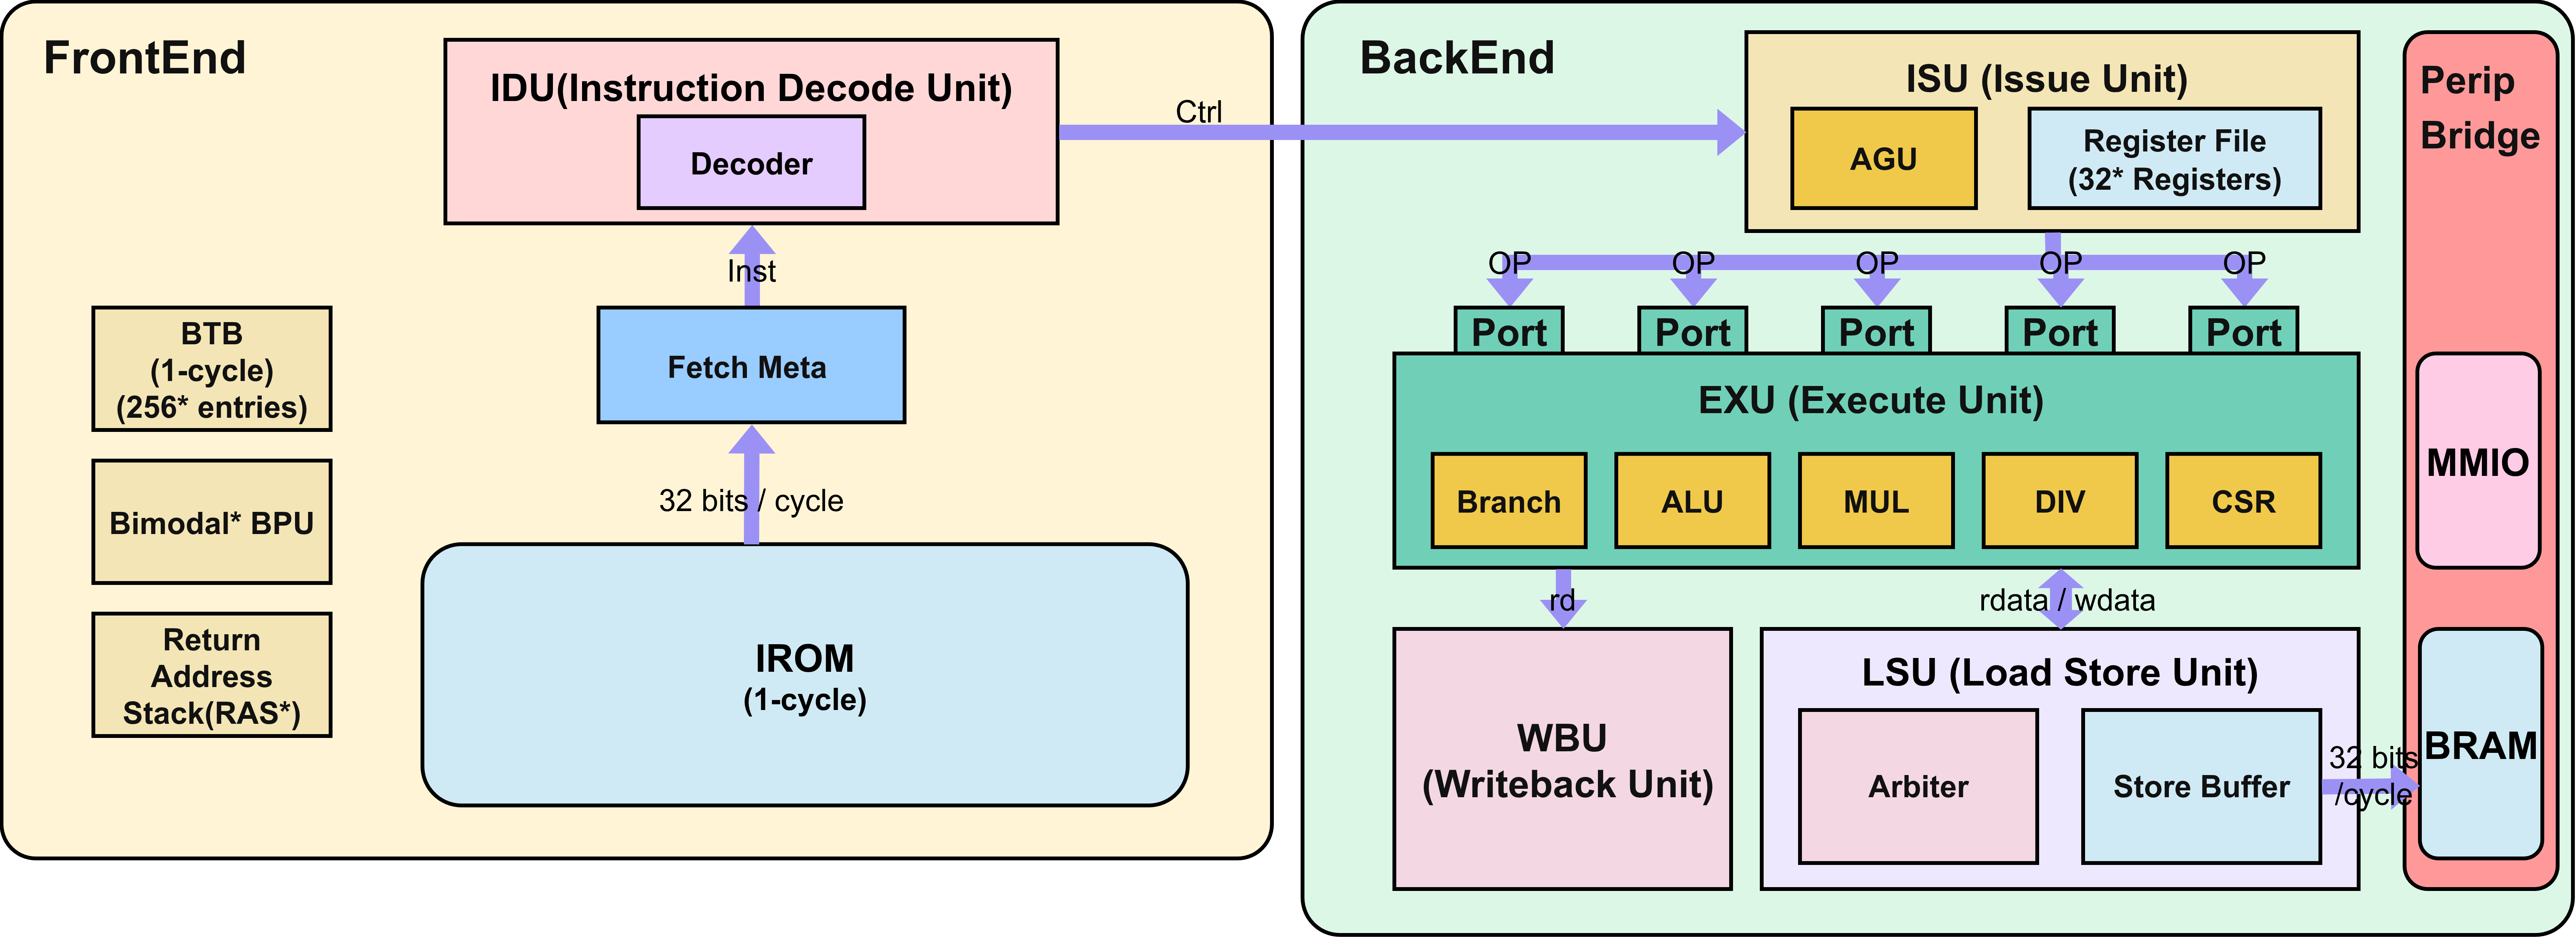
\includegraphics[width=\linewidth,height=0.5\textheight,keepaspectratio]{mundus_core_architecture_horizontal.png}
\caption{Mundus 核内模块总体关系}
\label{fig:core-overview}
\end{figure}

\subsection{硬件系统介绍}
\subsubsection{硬件整体介绍}
核心采用 Chisel 描述，并生成 SystemVerilog 与 FPGA IP、存储器和外设包装集成。
验证目标为 Xilinx Kintex-7，使用 Vivado 2023.2 进行综合、实现和比特流生成。
九级流水线将前端预测和同步取指、后端运算与数据返回分开组织，以降低单周期组合逻辑压力。
\subsubsection{机械设计介绍}
作品依托现有 FPGA 试验平台实现，不包含独立机壳、传动机构或机械装配设计。
\subsubsection{电路各模块介绍}
\paragraph{SoC 集成方式}

目前将处理器封装为赛方 \id{Core_cpu} 接口，连接 IROM、DRAM、LED、数码管、
SW、KEY 和计数器，图~\ref{fig:soc-framework} 给出系统连接。

\paragraph{核心接口}

当前处理器顶层采用 IROM 与 PERIP 两组直连 SoC 接口。
接口信号见表~\ref{tab:core-interface}。

\begin{table}[H]
  \centering
  \caption{当前 CPU 核接口}
  \label{tab:core-interface}
  \begin{adjustbox}{max width=\linewidth}
\begin{tabular}{P{2.8cm}C{3.0cm}C{1.5cm}P{6.2cm}}
    \toprule
    信号 & 相对 CPU 方向 & 位宽 & 说明 \\
    \midrule
    irom.addr & 输出 & 32 & 指令取址地址 \\
    irom.data & 输入 & 32 & IROM 当前返回的指令 \\
    perip.addr & 输出 & 32 & DRAM/外设访问地址 \\
    perip.wen & 输出 & 1 & 写请求有效 \\
    perip.mask & 输出 & 2 & byte/half/word 访问宽度编码 \\
    perip.wdata & 输出 & 32 & 写数据 \\
    perip.rdata & 输入 & 32 & DRAM/外设读数据 \\
    \bottomrule
  \end{tabular}
\end{adjustbox}
\end{table}

\paragraph{SoC 地址空间}\label{tab:address-space}

\begin{table}[H]
  \centering
  \caption{SoC 地址空间}
  \begin{tabularx}{\linewidth}{@{}P{1.7cm}P{5.2cm}P{1.1cm}X@{}}
    \toprule
    区域 & 地址范围 & 属性 & 说明 \\
    \midrule
    IROM & {\ttfamily\zihao{5}0x80000000--0x80003FFF} & 只读 & 16 KiB，当前周期读 \\
    DRAM & {\ttfamily\zihao{5}0x80100000--0x8013FFFF} & 读写 & 256 KiB，支持 1/2/4 byte \\
    SW & {\ttfamily\zihao{5}0x80200000--0x80200007} & 只读 & 仅 4 byte 对齐访问 \\
    KEY & {\ttfamily\zihao{5}0x80200010--0x80200013} & 只读 & 低 8 bit 有效 \\
    SEG & {\ttfamily\zihao{5}0x80200020--0x80200023} & 读写 & 七段数码管 \\
    LED & {\ttfamily\zihao{5}0x80200040--0x80200043} & 只写 & LED 显示 \\
    \id{COUNTER} & {\ttfamily\zihao{5}0x80200050--0x80200053} & 读写 & 起止计时控制 \\
    \bottomrule
  \end{tabularx}
\end{table}

\paragraph{指令集支持}

\begin{table}[H]
  \centering
  \caption{当前指令集支持情况}
  \label{tab:isa}
  \begin{tabularx}{0.96\textwidth}{P{2.5cm}X}
    \toprule
    类别 & 支持指令 \\
    \midrule
    RV32I 算术/逻辑 & \code{add, sub, addi, and, or, xor, andi, ori, xori, lui, auipc} \\
    RV32I 移位/比较 & \code{sll, srl, sra, slli, srli, srai, slt, sltu, slti, sltiu} \\
    RV32I 访存 & \code{lb, lh, lw, lbu, lhu, sb, sh, sw} \\
    RV32I 控制流 & \code{beq, bne, blt, bge, bltu, bgeu, jal, jalr} \\
    RV32M & \code{mul, mulh, mulhsu, mulhu, div, divu, rem, remu} \\
    Zicsr & \code{csrrw, csrrs, csrrc, csrrwi, csrrsi, csrrci} \\
    特权相关 & \code{ecall, mret}；\code{ebreak} 可被识别，尚不作为完整调试异常实现 \\
    \bottomrule
  \end{tabularx}
\end{table}

\paragraph{总体结构}

\cpuname{} 采用顺序、单发射、单提交结构，每周期最多接收并提交一条指令。
前端分为 IF1、IF2、ID、ISS，后端分为 EX1、EX2、EX3、EX4、WB，具体功能见图~\ref{fig:current-pipeline} 及下文。

\begin{figure}[htbp]
\centering

\includegraphics[width=\textwidth,height=0.68\textheight,keepaspectratio]{MundusPipeline.png}
\caption{当前 \cpuname{} 九阶段单发射处理器结构}
\label{fig:current-pipeline}
\end{figure}

九级流水线依次划分为 IF1、IF2、ID、ISS、EX1、EX2、EX3、EX4 和 WB。IF1 负责 PC 选择、预测请求和同步 IROM 地址发起，IF2 将一拍后返回的指令与 PC、顺序 PC 及预测元数据对齐；ID 完成译码和立即数生成，ISS 完成同步 RegisterFile 读取、相关性检查、旁路选择及访存地址生成；EX1 分别开始执行 ALU、Branch、CSR 运算、访存、乘除法流水线，在 EX1 末期返回 ALU 结果，EX2 接收 LSU 返回的 Load Word 结果，EX3 开始分支预测检测并接收 LSU 返回的 Load Half/Byte 结果，EX4 向 LSU 提供 Store data，并广播分支预测错误的 flush 信号，用于冲刷流水线寄存器以及写入 CSR、存储器操作；WB 作为统一顺序提交与 RegisterFile 写回点。

控制冒险发生时清空相应阶段流水线寄存器上的错误路径指令；普通数据相关在 ISS 阶段互锁并向 EX1 注入气泡；除法结果未完成时则冻结需要保持精确顺序的流水级。

\paragraph{RTL 前端设计}

当前前端由 PC 选择逻辑、BPU、同步 IROM、取指元数据寄存器以及 IF/ID 输出通路组成，
如图~\ref{fig:frontend-architecture} 所示。BPU 以 Bimodal 预测器判断跳转方向，
通过 BTB 保存历史跳转目标，并可选配返回地址栈 RAS 预测函数返回地址。PC 用于驱动
IROM 取指并生成对应的请求元数据；IROM 返回指令后，与 \id{FetchMeta} 中保存的
PC 及预测信息对齐，共同组成取指响应并送入 IDU。

RAS 对函数调用与返回较频繁的程序具有较明显的预测收益，\textbf{但对于此类控制流较少的程序，
准确率改善可能较为有限；与此同时，RAS 及其更新、选择逻辑也会增加一定的硬件资源和
布局布线负担}。因此,本设计将 RAS 实现为由 \code{CONFIG_BRANCH_RAS} 控制的\textbf{可选配置}。
启用该配置时，生成的可综合 RTL 包含 RAS、返回指令标记以及相应的更新和目标选择逻辑；
关闭该配置时，上述模块、接口和数据通路均不参与硬件例化，BPU 仅使用 Bimodal 与 BTB
完成分支预测。

上述预测参数可通过 menuconfig 界面统一配置，如图~\ref{fig:branch-menuconfig} 所示。
设计者可以选择分支预测策略，设置 BTB 索引宽度和 Bimodal 计数器位宽，并独立控制
RAS 是否启用及其索引宽度。配置结果会在生成 RTL 时生效，从而在预测能力与硬件开销
之间进行取舍。

\begin{figure}[htbp]
  \centering
  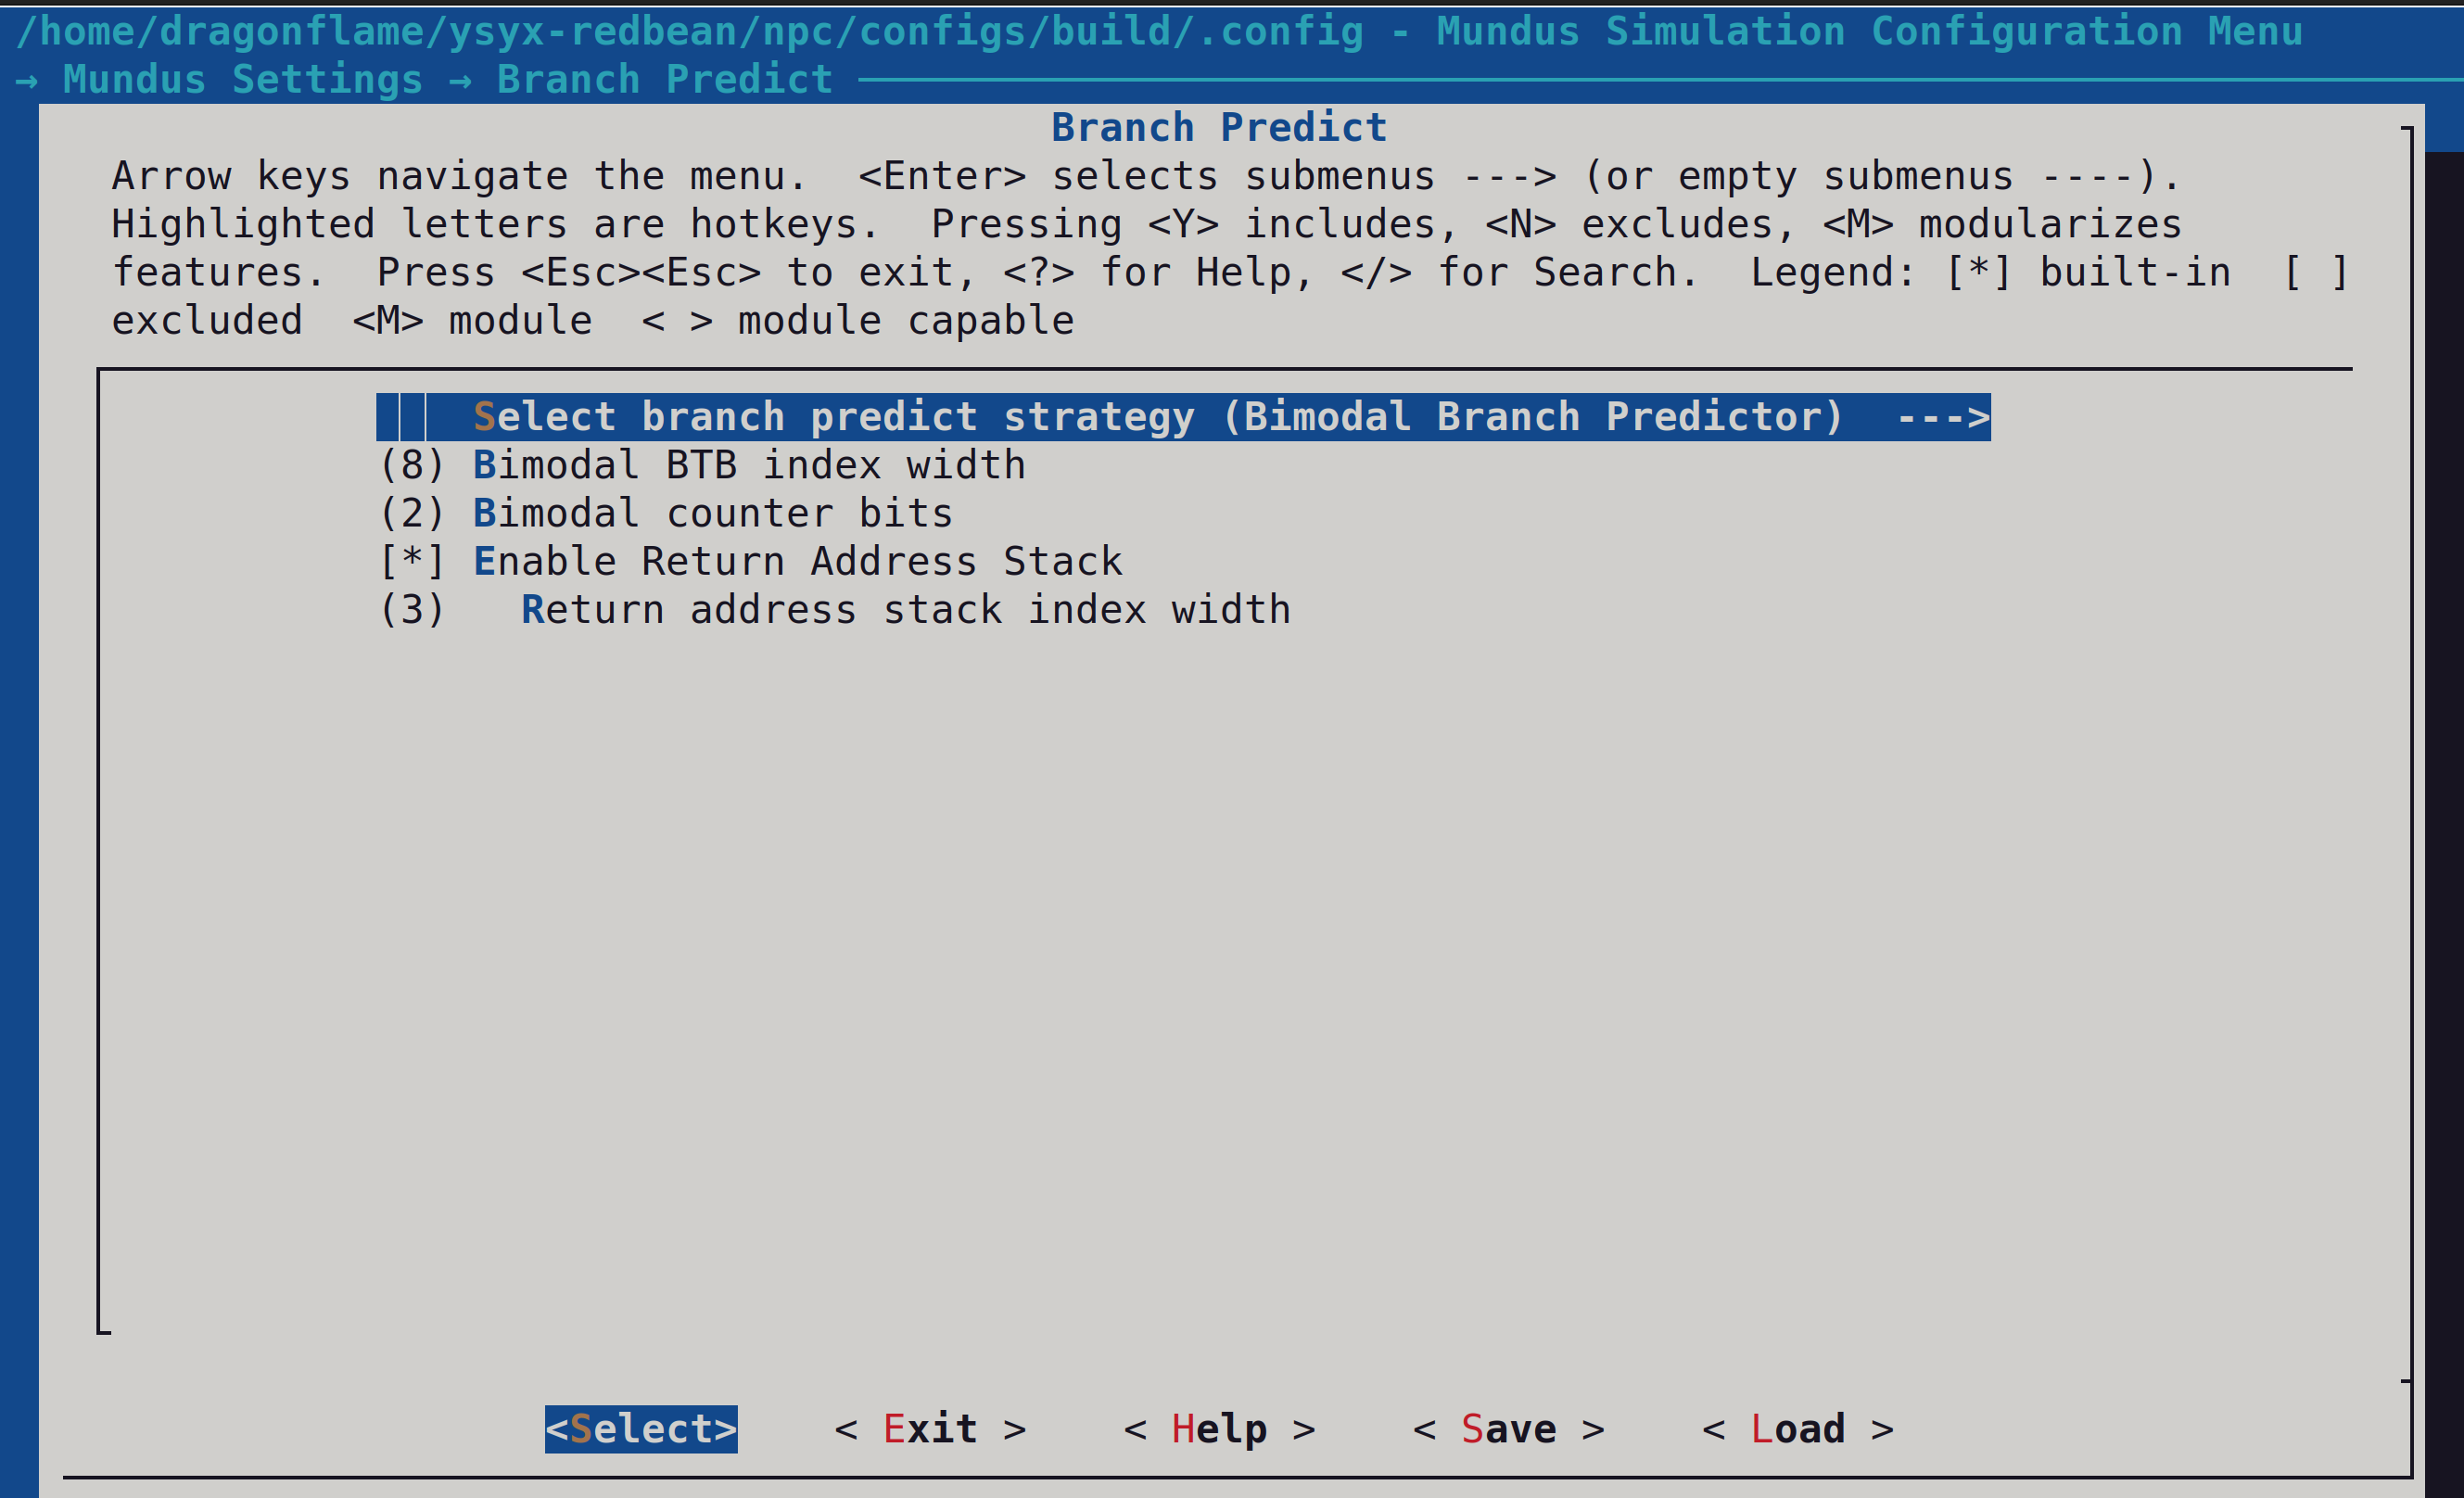
\includegraphics[width=0.94\linewidth,height=0.68\textheight,keepaspectratio]{menuconfig_branch_predict.png}
  \caption{分支预测单元的 menuconfig 配置界面}
  \label{fig:branch-menuconfig}
\end{figure}

\begin{figure}[htbp]
  \centering
  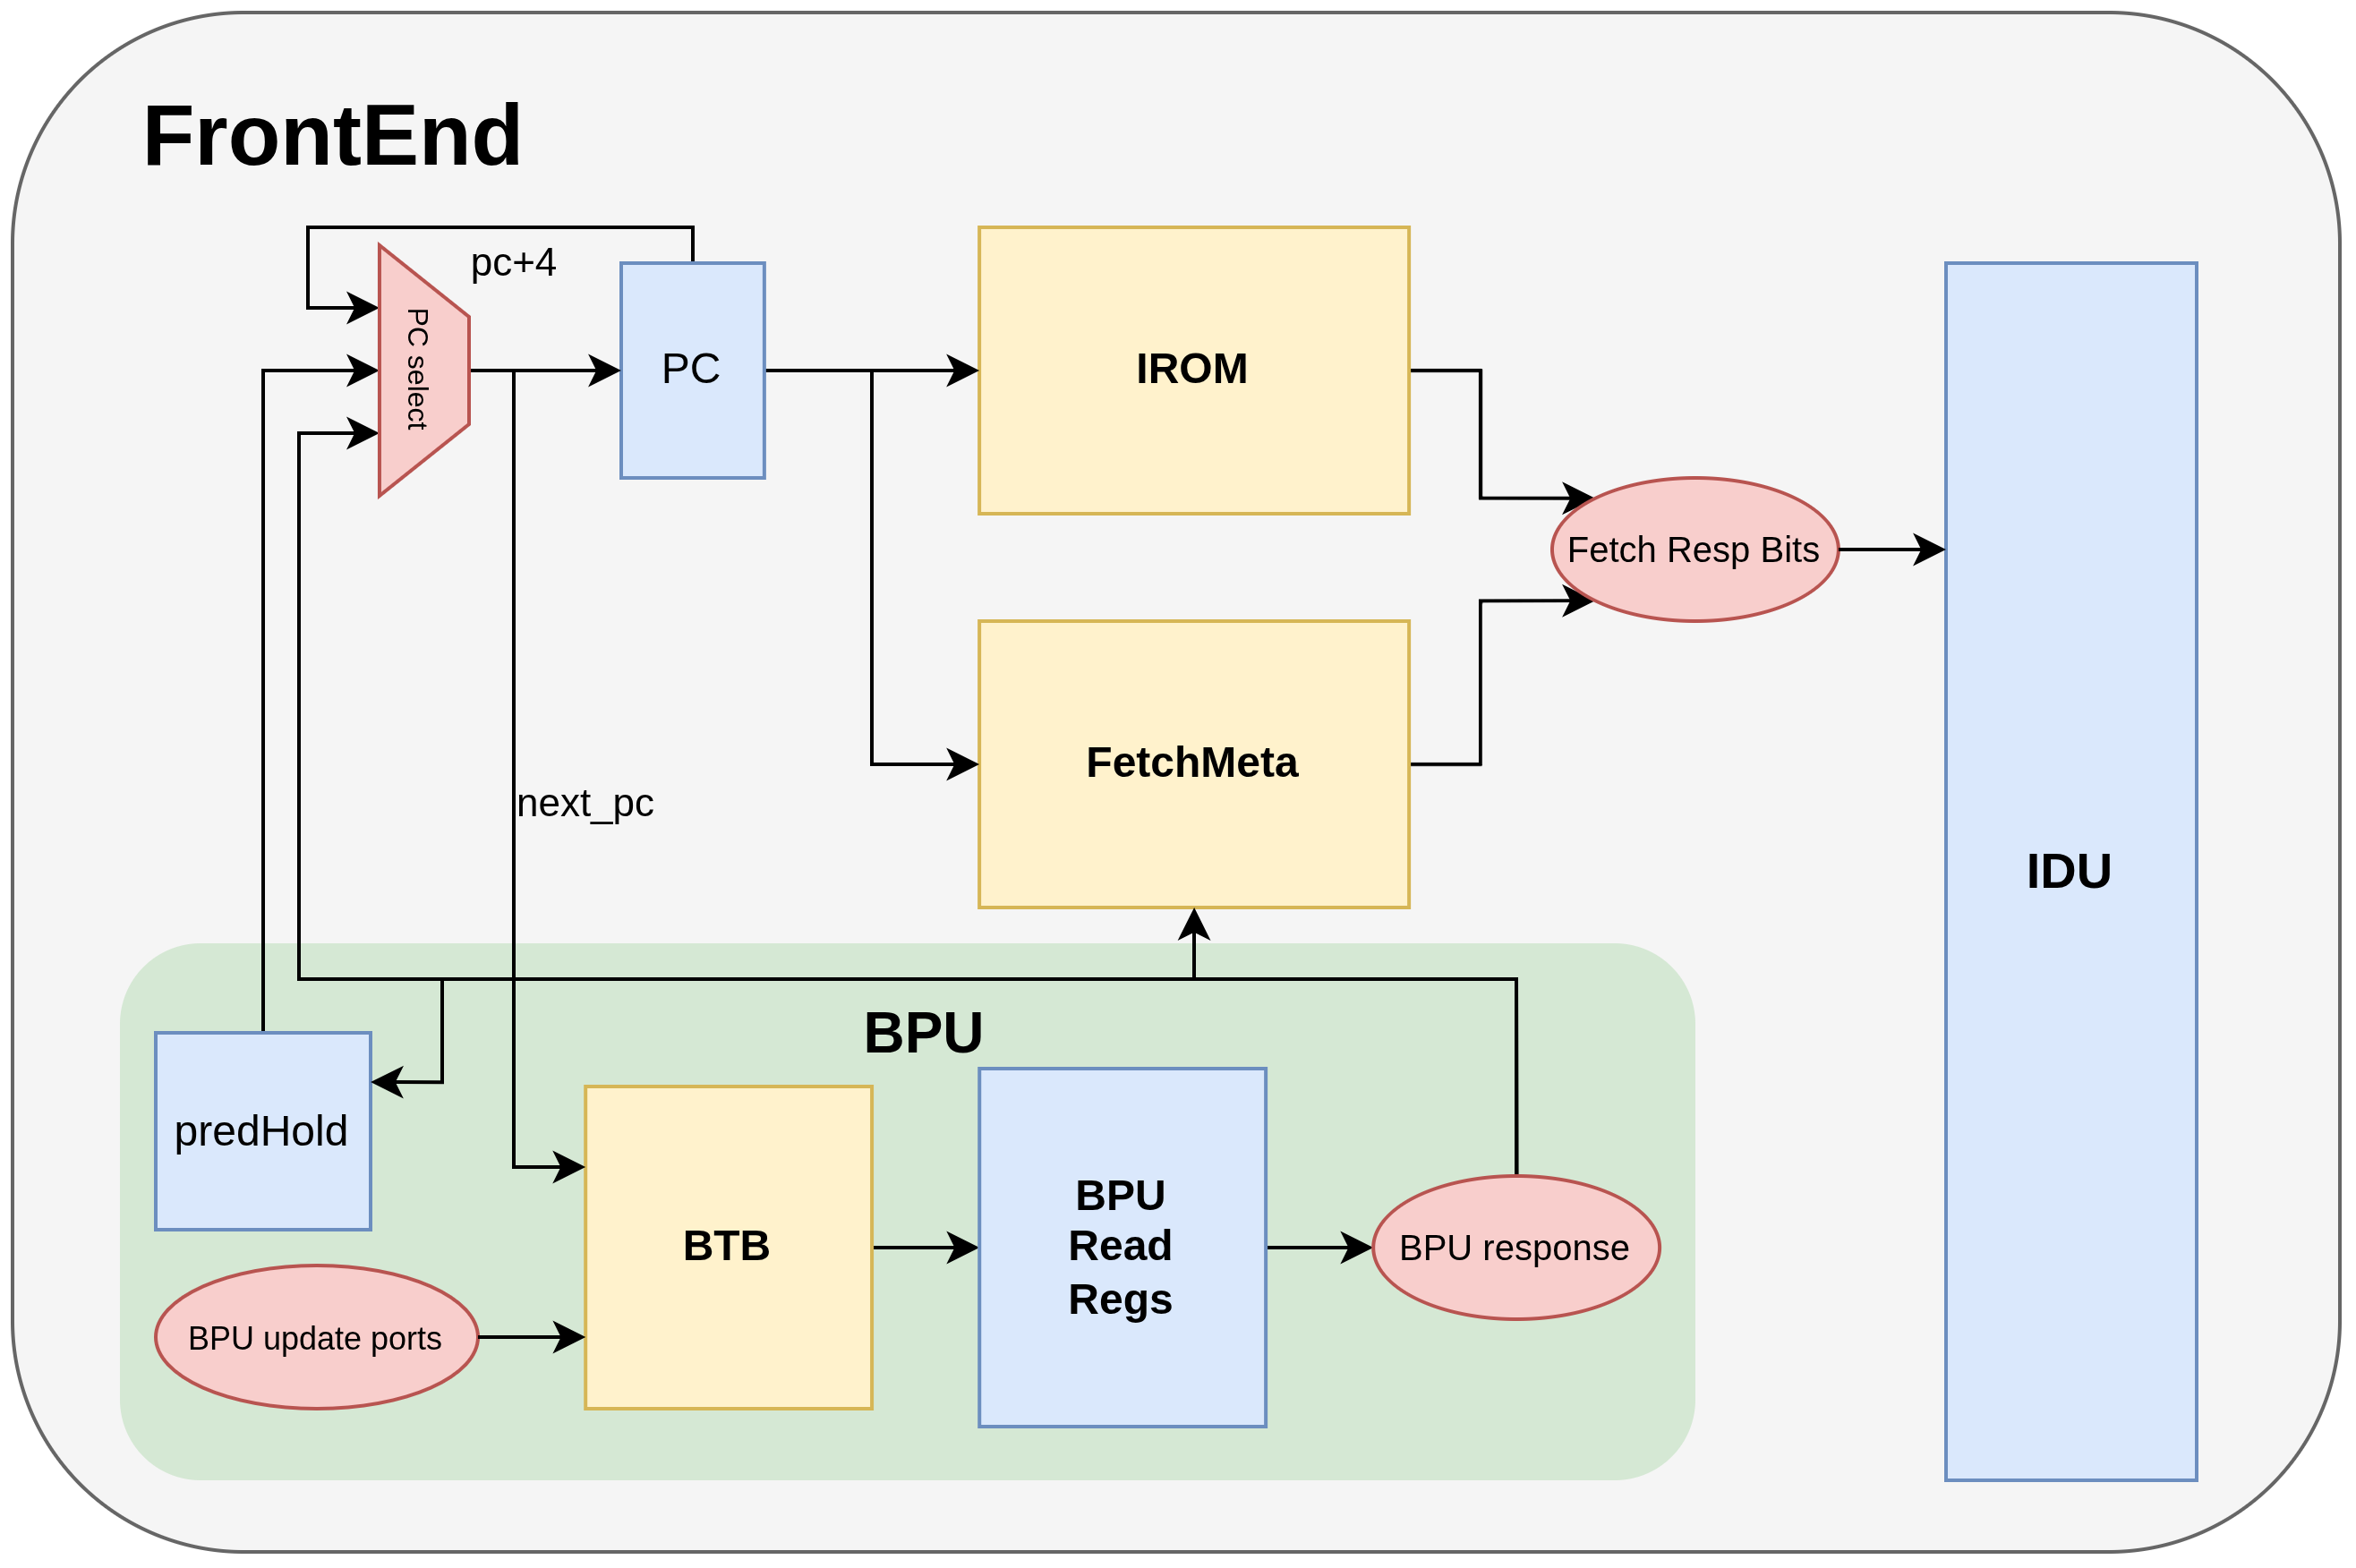
\includegraphics[width=0.98\linewidth,height=0.68\textheight,keepaspectratio]{front_arch.png}
  \caption{当前 RTL 前端总体结构}
  \label{fig:frontend-architecture}
\end{figure}

\subparagraph{分支预测单元 BPU}

\Needspace{4\baselineskip}
\medskip
\noindent\textbf{Bimodal 方向预测}\par

当前 BPU 使用 Bimodal 预测器学习分支的历史跳转倾向。每个已记录的控制流指令对应一个
2 bit 饱和计数器 \id{counter}，计数器的最高位给出方向预测：SNTK 和 WNTK 预测
不跳转，WTK 和 STK 预测跳转。Bimodal 的方向状态在物理实现上与 BTB 表项一一对应，
不再单独设置 PHT，从而复用同一组索引和读出寄存器。

\begin{table}[H]
  \centering
  \caption{Bimodal 2 bit 饱和计数器状态}
  \label{tab:bimodal-counter}
  \begin{adjustbox}{max width=\linewidth}
\begin{tabular}{ccc}
    \toprule
    状态 & 编码 & 预测倾向 \\
    \midrule
    SNTK & \id{2'b00} & 强不跳转 \\
    WNTK & \id{2'b01} & 弱不跳转 \\
    WTK  & \id{2'b10} & 弱跳转 \\
    STK  & \id{2'b11} & 强跳转 \\
    \bottomrule
  \end{tabular}
\end{adjustbox}
\end{table}

EX1 得到真实控制流结果后，将实际方向反馈给预测器。对应索引项已经有效时，计数器根据
实际结果向 STK 或 SNTK 饱和更新；空表项首次记录一次实际跳转时，计数器从 WTK
开始。复位时计数器初始化为 WNTK，使尚未完成训练的表项倾向于预测不跳转。

\Needspace{4\baselineskip}
\medskip
\noindent\textbf{返回地址栈 RAS}\par

间接跳转指令 \code{jalr} 的目标地址由寄存器操作数决定，仅依赖 BTB 中上一次保存的
目标难以稳定预测函数返回。为此，BPU 增加可选配置返回地址栈 RAS，专门记录尚未返回的函数
调用地址。当前 \id{RAS_WIDTH=3}，栈深度为 $2^3=8$。
RAS \textbf {采用移位式栈结构}：
执行 push 时，原有表项依次向栈底移动，并将新的返回地址写入 \code{stack[0]}；
执行 pop 时，后续表项依次向栈顶移动。因此，\code{stack[0]} 始终保存当前栈顶地址，
预测端可以直接读取该地址，无需通过栈指针对多个表项进行动态选择。

IDU 根据 \code{jal}/\code{jalr} 的
\code{rd} 和 \code{rs1} 字段生成 RAS 更新提示。按照 RISC-V 的约定，
\code{x1} 和 \code{x5} 均可作为链接寄存器：指令通过链接寄存器保存
\id{PC+4} 时产生 \id{ras_push}，将新的返回地址压入 RAS；\code{jalr}
使用链接寄存器作为跳转源、但不通过同一寄存器保存新返回地址时产生
\id{ras_pop}。若 \code{jalr} 分别使用两个不同的链接寄存器作为源和目的，
则同时产生 \id{ras_pop} 和 \id{ras_push}，实现协程切换所需的先弹出旧返回
地址、再压入新返回地址。

BTB 表项使用 \id{is_return} 标记已识别的返回指令。预测端在 BTB 命中、
\id{is_return} 有效且 RAS 非空时，将该指令直接预测为跳转，并使用 RAS 栈顶覆盖
BTB 中保存的历史目标；若 RAS 为空，则退回普通 Bimodal 与 BTB 的预测结果。于是返回
预测命中条件及最终选择为
\begin{equation}
  \begin{aligned}
    \mathrm{return\_hit}
      &= \mathrm{pred\_is\_return}
         \land \mathrm{ras\_top\_valid}, \\
    \mathrm{pred\_taken}
      &= \mathrm{return\_hit}
         \lor \mathrm{bimodal\_taken}, \\
    \mathrm{pred\_target}
      &= \begin{cases}
           \mathrm{ras\_top}, & \mathrm{return\_hit},\\
           \mathrm{btb\_target}, & \text{otherwise}.
         \end{cases}
  \end{aligned}
\end{equation}

\Needspace{4\baselineskip}
\medskip
\noindent\textbf{BTB 表项与命中更新}\par

BTB 采用直接映射结构，当前配置 \id{BTB_WIDTH=8}，共有 $2^8=256$ 个表项。
每个表项包含 \id{valid}、\id{tag}、历史跳转目标 \id{target}、Bimodal 的 2 bit
\id{counter} 以及返回指令标志 \id{is_return}，相关阵列被约束为 Distributed RAM。
取指 PC 按 4 字节对齐，\id{PC[9:2]} 用作索引，\id{PC[31:10]} 用作 tag；索引
选出候选表项后，再由 valid 和 tag 比较确认其是否属于当前 PC，基本结构如图
~\ref{fig:bimodal-btb} 所示。

\begin{figure}[htbp]
  \centering
  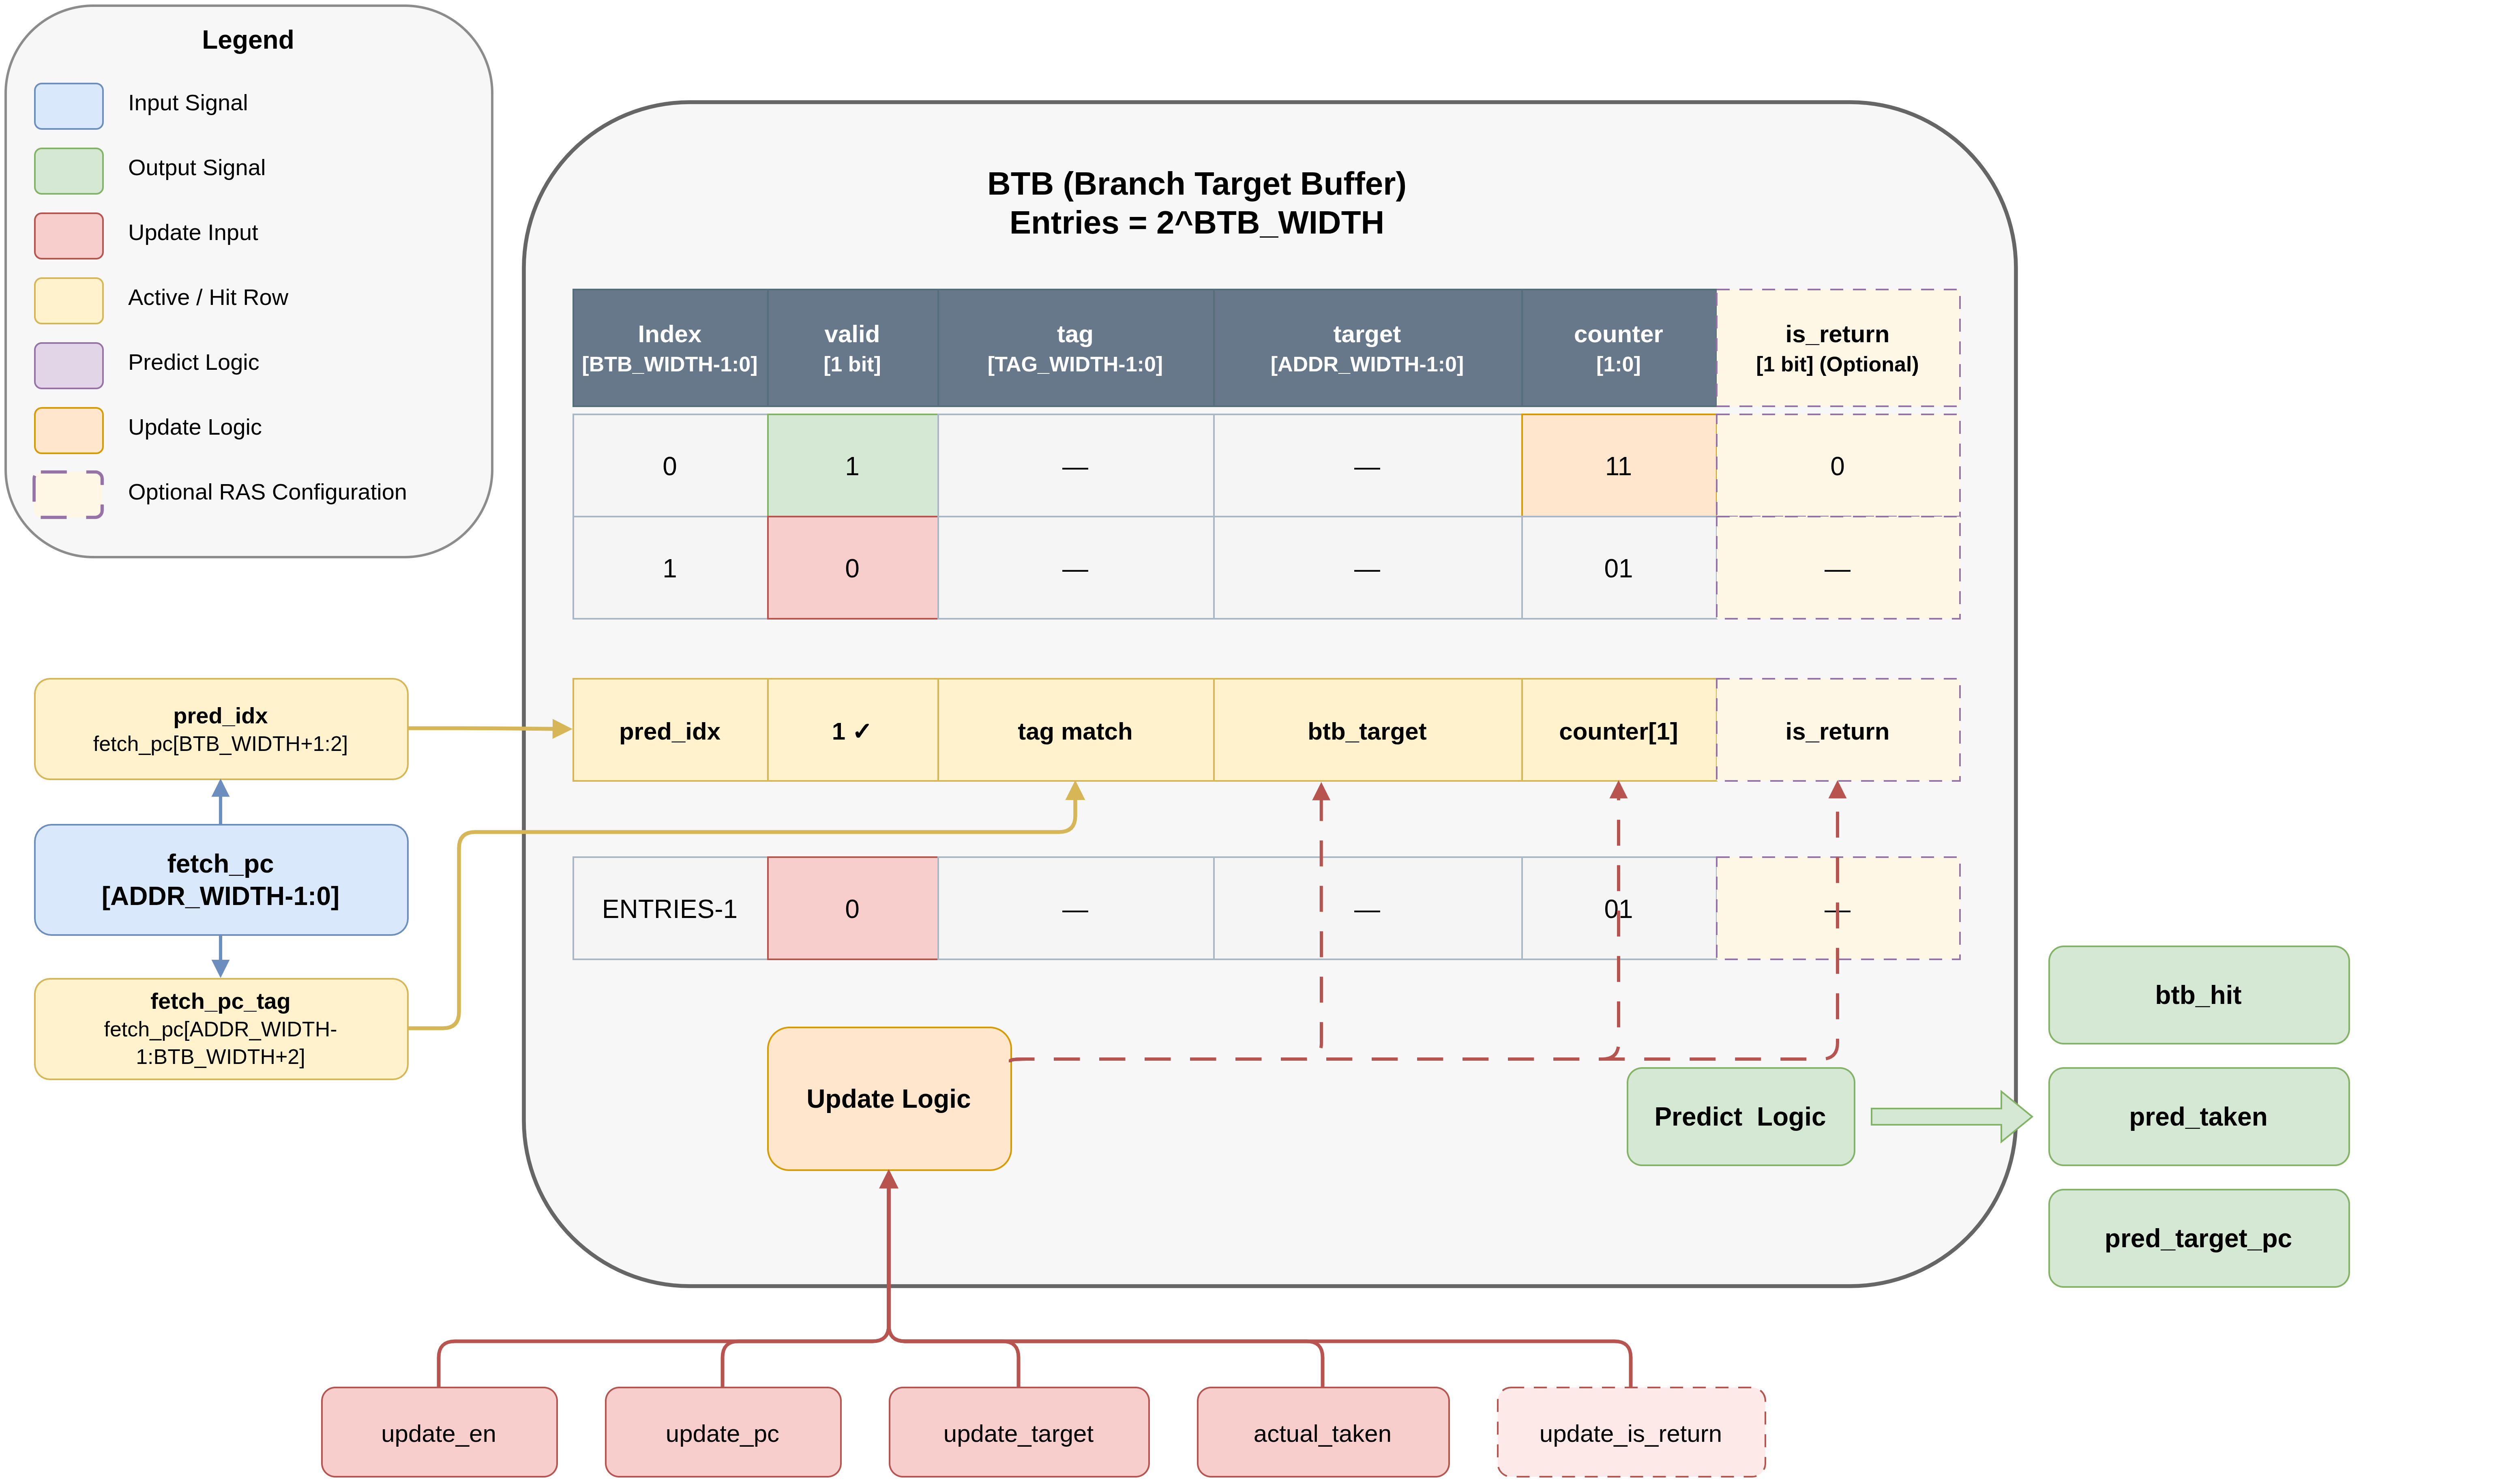
\includegraphics[width=0.96\linewidth,height=0.68\textheight,keepaspectratio]{btb.png}
  \caption{Bimodal、BTB 与 RAS 预测选择结构}
  \label{fig:bimodal-btb}
\end{figure}

预测时，\id{fetch_pc} 同时产生索引和 tag。只有候选表项有效且 tag 相等时才命中；
普通控制流指令在命中后以计数器最高位判断方向，并使用表项 target 作为跳转目标：
\begin{equation}
  \begin{aligned}
    \mathrm{pred\_hit}
      &= \mathrm{valid\_r}
         \land (\mathrm{tag\_r}=\mathrm{pred\_tag\_r}), \\
    \mathrm{bimodal\_taken}
      &= \mathrm{pred\_hit}
         \land \mathrm{counter\_r}[1], \\
    \mathrm{pred\_is\_return}
      &= \mathrm{pred\_hit}
         \land \mathrm{is\_return\_r}.
  \end{aligned}
\end{equation}
未命中或最终预测不跳转时，IFU 选择 \id{PC+4}。EX1 确认控制流指令实际跳转后，
BTB 写入 valid、tag、target 和 \id{is_return}；同时按实际方向训练对应的 Bimodal
计数器。复位时所有 valid 清零、counter 初始化为 WNTK；tag、target 和
\id{is_return} 不复位，其无效内容由 valid 屏蔽。控制冒险通过比较预测下一 PC 与
真实下一 PC 判断，两者不一致时由 HZU 发出 redirect。

\Needspace{4\baselineskip}
\medskip
\noindent\textbf{一拍预测与提前查询}\par

若在一个周期内依次完成预测表读取、tag 命中比较、counter 方向判断以及 target 与
\id{PC+4} 的选择，整条组合逻辑会直接连接到 PC寄存器输入，路径较长。\textbf{为缩短该路径}，
将预测表读出结果寄存：第 $N$ 拍输入要预测的 PC 和
请求使能，时钟沿锁存请求 PC 及表项的 valid、tag、target、counter 和
\id{is_return}，
第 $N+1$ 拍输出预测响应，使预测表阵列的读取不再位于同拍的 PC 更新路径中。

一拍接口也意味着，若直接查询当前 PC，必须到下一拍才能确定预测取指地址，连续取指会
产生气泡。当前 IFU 因而采用提前查询。设本拍 PC 为 $P$，BPU 已返回 $P$ 的预测，
IFU 组合得到候选下一地址 $Q$：
\begin{equation}
  Q=\begin{cases}
    \mathrm{pred\_target}(P), & \mathrm{pred\_taken}(P),\\
    P+4, & \text{otherwise}.
  \end{cases}
\end{equation}
当本拍取指请求被接受时，PC 在时钟沿更新为 $Q$，同时 BPU 查询端直接接收 $Q$，而
IROM 仍接收当前地址 $P$。下一拍 BPU 对 $Q$ 的预测与已经更新为 $Q$ 的 PC 对齐，
可以继续计算再下一地址。这样一拍预测延迟被流水隐藏，稳态仍可每周期接受一条取指
请求。

完成一拍流水化后，预测到 PC 寄存器的组合路径仍然较长，其主要经过：BTB/Bimodal
读出寄存器 $\rightarrow$ valid/tag 命中比较、counter 方向判断与返回类型判断
$\rightarrow$ RAS 栈顶目标覆盖
$\rightarrow$ 当前响应与暂存预测选择
$\rightarrow$ 预测目标与 $\mathrm{PC}+4$ 选择
$\rightarrow$ PC 寄存器输入。该路径虽然不再包含预测表阵列的读取，但仍包含 tag 比较、
RAS 选择、多级选择和 32 bit 加法，仍是前端综合与布局布线时需要重点观察的关键路径。

\Needspace{4\baselineskip}
\medskip
\noindent\textbf{预测保持与重定向清理}\par

预测保持机制用于解耦 BPU 响应与 IFU 取指请求：BPU 的响应只在对应周期有效，但 IFU
可能因后端停顿而暂时无法发出请求。若不保存该响应，恢复取指时会
丢失已经得到的预测方向和目标，并直接进行顺序地址选择，\textbf{很有可能会导致预测错误，使IPC降低}。

为了解决上面提到的问题，添加了
\id{predHoldValid}、\id{predHoldTaken} 和 \id{predHoldTarget}寄存器来保存这一次预测。
后续请求恢复时优先使用暂存结果，并在请求被接受后清除暂存有效位。固定的一拍响应保证了
同一时刻最多只有一个需要暂存的预测。
在重定向的时候，redirect信号用于防止错误路径的预测在流水线冲刷后再次生效。当\id{redirect} 拉高时，IFU
在当拍禁止新请求并清除预测暂存；下一拍也不会产生与旧请求对应的有效 BPU 响应，因而
旧路径的预测方向和目标不会被重新消费。

\subparagraph{取指单元 IFU 与同步 IROM}

指令存储器采用的是 Block Memory Generator 生成的单端口 ROM，有一拍的读延迟，因此 IROM 是同步读：
第 $N$ 拍给出地址 $P$，第 $N+1$ 拍才得到
inst$(P)$。IFU 使用 \id{fetchRespValid} 表示这一拍返回是否属于有效请求，并在
\id{fetchRespMeta} 中保存请求 PC、顺序 PC、预测方向和预测目标。IROM 数据返回后，
再与这组元数据组合成 IF/ID payload，避免使用已经前进后的当前 PC。

表~\ref{tab:frontend-timing} 给出无 stall、无 redirect 且下游可接收时的稳态时序。
其中 $Q$ 是根据 $P$ 的预测得到的下一地址，$R$ 是根据 $Q$ 的预测得到的再下一地址。

\begin{table}[H]
  \centering
  \caption{BPU 提前预测与同步 IROM 的稳态对齐}
  \label{tab:frontend-timing}
  \begin{tabularx}{0.98\textwidth}{P{3.0cm}YYY}
    \toprule
    信号/动作 & 第 $N$ 拍 & 第 $N+1$ 拍 & 第 $N+2$ 拍 \\
    \midrule
    PC 寄存器 & $P$ & $Q$ & $R$ \\
    IROM 地址 & $P$ & $Q$ & $R$ \\
    IROM 输出 & 前一请求数据 & inst$(P)$ & inst$(Q)$ \\
    BPU 请求 PC & $Q$ & $R$ & 下一候选地址 \\
    BPU 有效响应 & pred$(P)$ & pred$(Q)$ & pred$(R)$ \\
    响应元数据 & 准备 $P$ & $P$ 有效，准备 $Q$ & $Q$ 有效，准备 $R$ \\
    IROM 响应组合 & 前一请求 & inst$(P)$ 与 $P$ 的元数据 & inst$(Q)$ 与 $Q$ 的元数据 \\
    \bottomrule
  \end{tabularx}
\end{table}

目前使用一个响应槽FetchMeta连接同步 IROM 与 IF/ID 接口。
\id{fetchRespValid} 表示响应槽中保存的请求元数据以及
当前 IROM 输出是否有效。当响应槽为空，或其中的指令正在被下游接收时，IFU
允许同拍消费旧响应并发出下一次请求，因此如果下游持续 ready 时，前端仍可
保持每周期一次取指请求。

当 \id{fetchRespValid} 有效但下游停顿时，IFU会停止新请求和 PC 更新，
并将 IROM 地址保持为响应槽中的PC，使同步 ROM 输出的
指令与已保存的 PC、顺序 PC 和预测信息保持一致，直到该响应被下游接收。数据路径为
PC 寄存器 $\rightarrow$ IROM 地址选择 $\rightarrow$ BRAM 同步输出
$\rightarrow$ 指令与 \id{fetchRespMeta} 组合 $\rightarrow$ IF/ID 接口。
单响应槽结构的关键控制路径为下游 \id{ready} 与 \id{fetchRespValid}
$\rightarrow$ \id{respSlotHolding} $\rightarrow$ \id{fetchReqFire}
$\rightarrow$ PC 写使能、BPU 请求有效以及响应元数据更新。

当预测错误需要重定向时，优先级高于正常取指，IFU 会禁止新请求、屏蔽 IF/ID 输出，
并将 PC 更新为 HZU 给出的真实下一地址，同时清除 \id{fetchRespValid}来保证暂存数据无效。下一拍 IFU 从
重定向地址重新发起取指，旧路径响应因有效位已清除而不会再次成为有效事务。

\subparagraph{译码单元 IDU}

IDU 从 IF/ID 接口接收 32 bit 指令，解析 opcode、rd、rs1、rs2 与 CSR 地址，并按
R、I、S、B、U、J 和 CSR 格式生成立即数。集中式译码表同时生成 ALU 操作数选择与
操作码、BRU/MDU/CSR 控制、寄存器写使能、访存方向、访存宽度、load 符号扩展方式，
以及源操作数最晚需求时刻等控制信息。PC、\id{snpc} 和分支预测结果不在 IDU 中
重新计算，而是随 ID/ISS payload 继续传递，供后续 BRU 校验预测结果。

启用RAS 后，IDU 还根据 \code{jal}/\code{jalr} 的寄存器字段
生成 RAS 更新提示。按照 RISC-V 对链接寄存器 \code{x1} 和 \code{x5} 的约定，
\code{jal} 或 \code{jalr} 写入链接寄存器时置位 \id{ras_push}；\code{jalr} 从
链接寄存器读取返回地址，并且目的寄存器不是同一个链接寄存器时置位 \id{ras_pop}。
若 \code{jalr} 的源、目的分别使用不同的链接寄存器，则两个信号同时置位，对应协程
切换所需的先 pop 后 push。IDU 只产生提示，不在译码阶段直接修改 RAS，以免错误路径
指令过早改变预测器状态。

\paragraph{RTL 后端设计}

\begin{figure}[htbp]
  \centering
  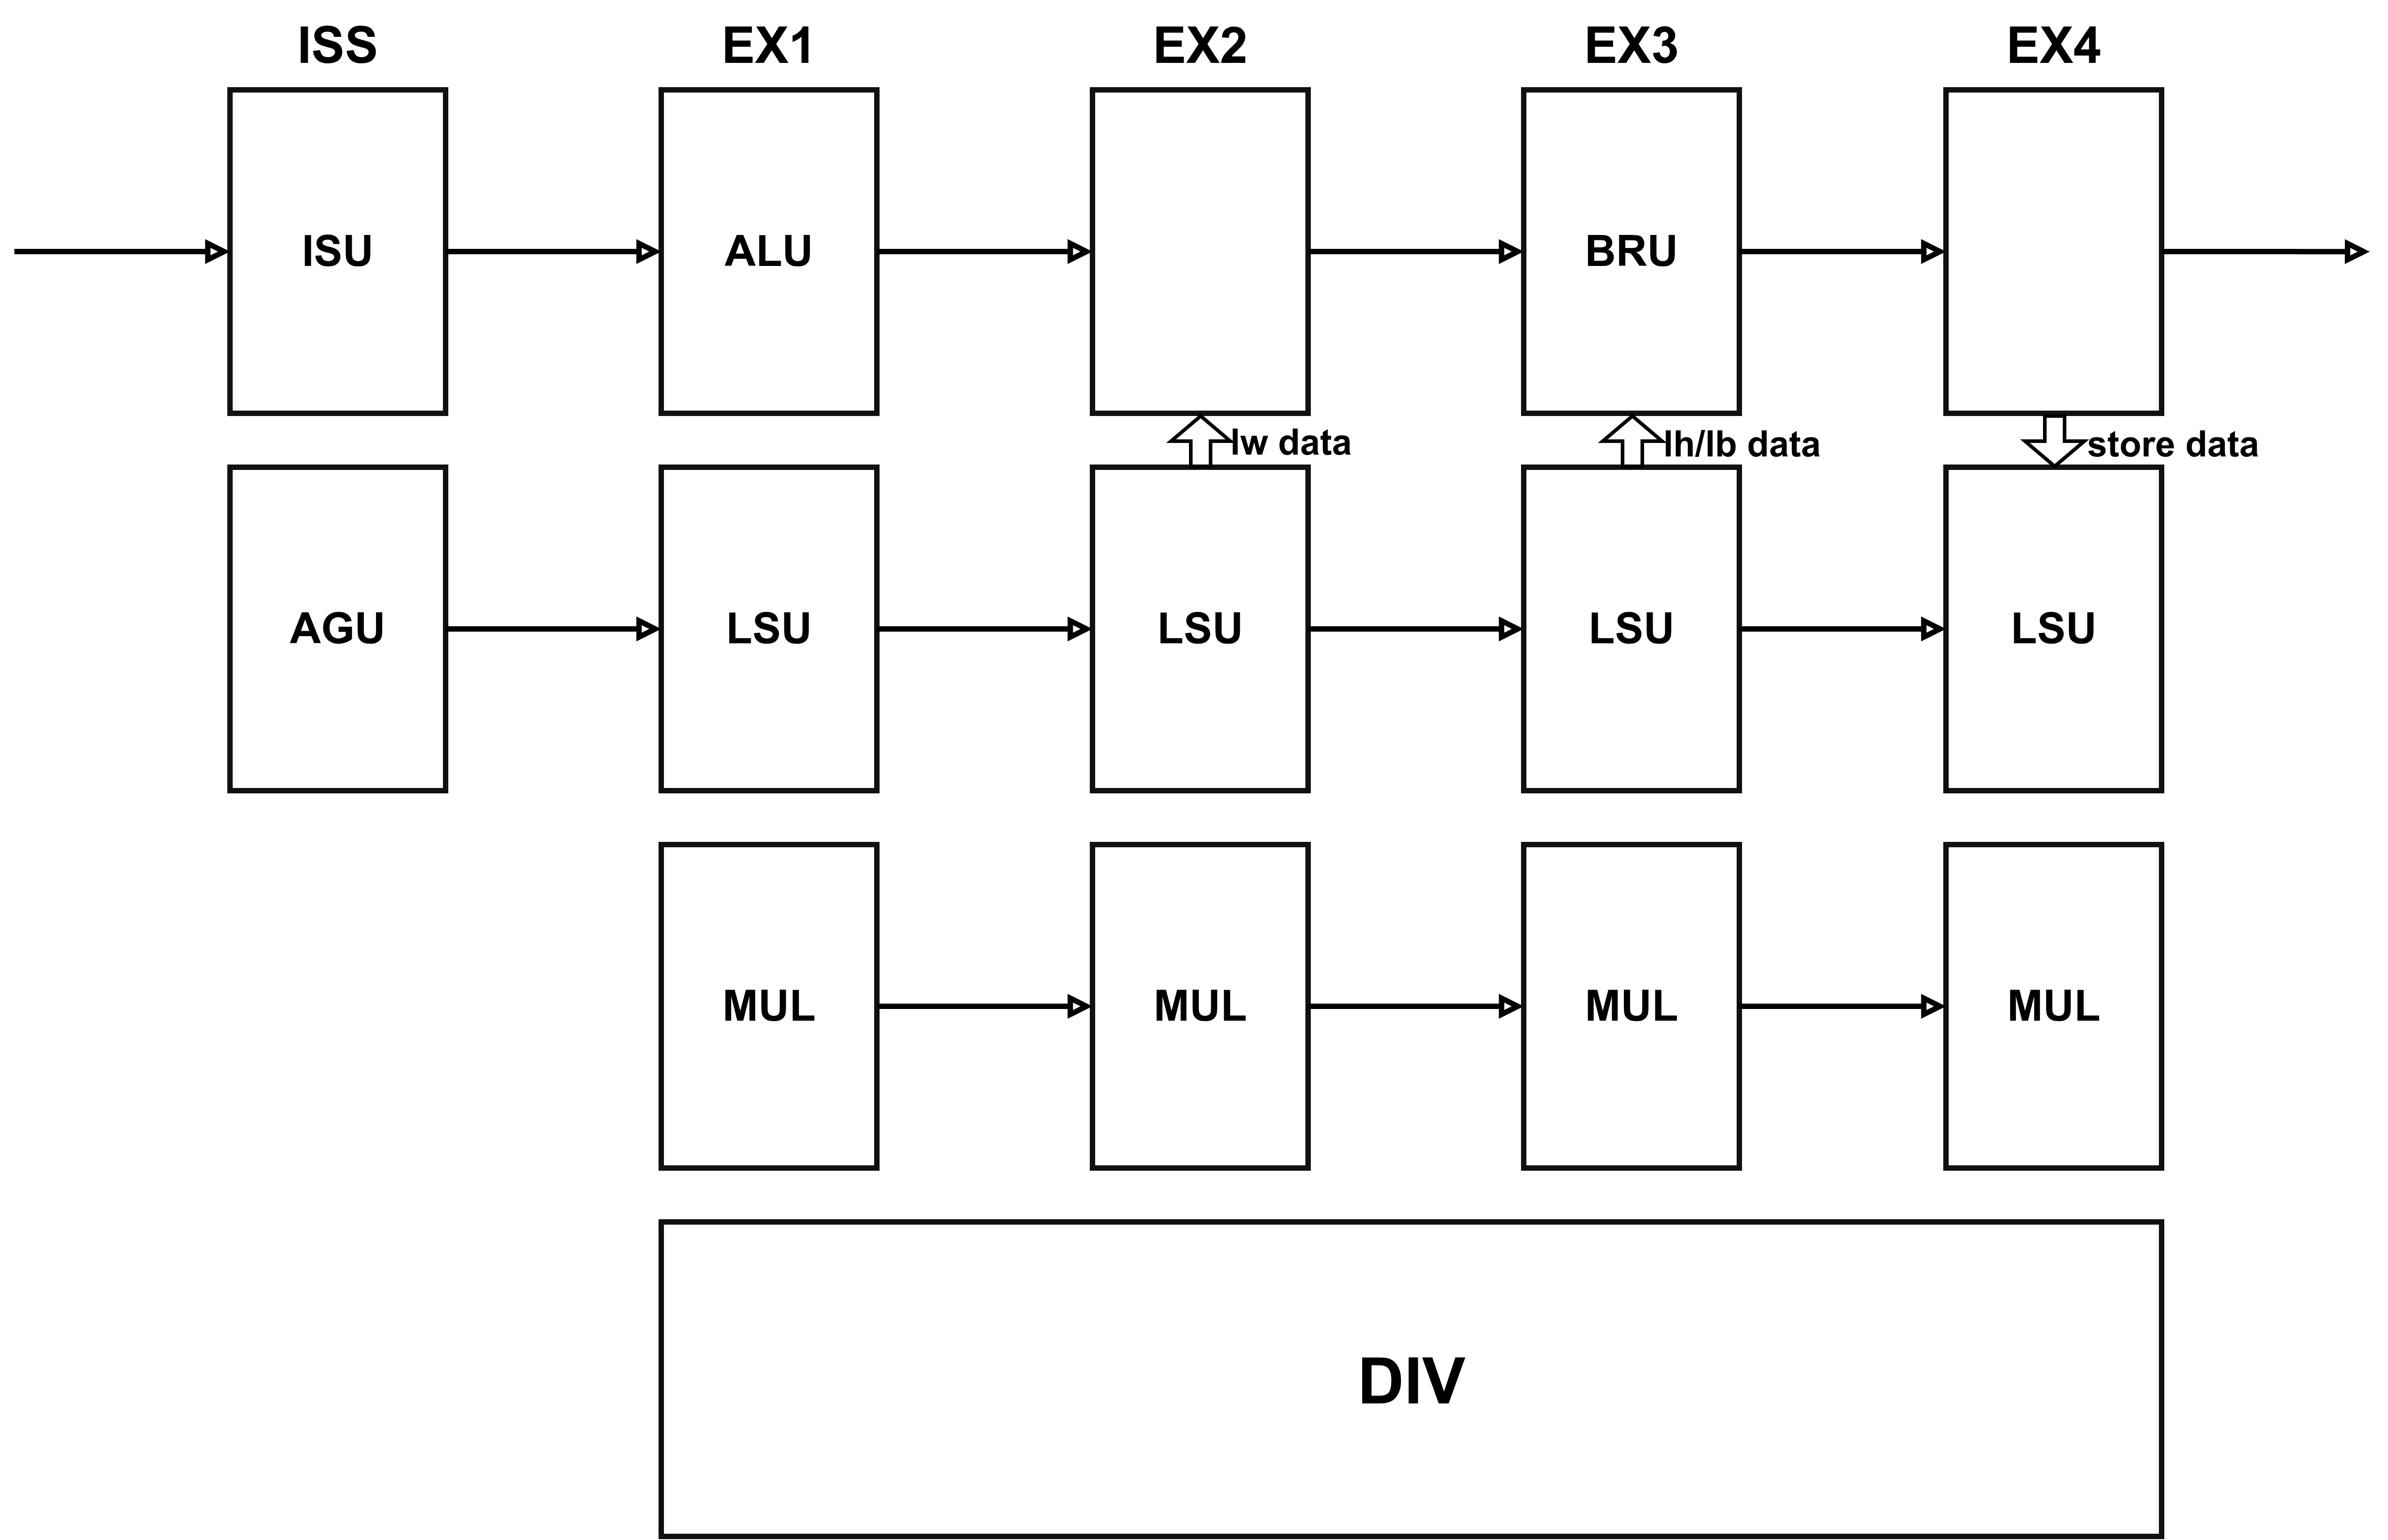
\includegraphics[width=\textwidth,height=0.68\textheight,keepaspectratio]{execution_pipeline.png}
  \caption{后端流水线架构}
  \label{fig:backend_pipeline}
\end{figure}

\subparagraph{发射与旁路单元 ISU}

ISU 负责 RegisterFile 旁路修正、数据相关检查和发射。ISU 的 interlock 信号，为 ISS 流水线阶段自锁信号，依据冒险在哪一流水线阶段产生，生产者能否满足消费者的需求而生成。（旁路及冒险相关内容，在第~\ref{subsec:bypass}~小节详细阐述）RegisterFile 的读地址通常由 ID 阶段提前提供，使同步读数据在指令进入 ISS 时对齐；若 ISS 因相关或除法未完成执行而停顿，则读地址保持当前指令，避免寄存器值错位。

本设计将访存地址的计算提前到 ISS 阶段，这虽然会导致 AGU 无法旁路 EX1 的数据，产生一个周期的 use-load stall，但是可以减少一个周期的 load-use stall。根据我们对汇编代码的分析，use-load stall的发生频率，往往比 load-use stall 要低。

\begin{figure}[htbp]
  \centering
  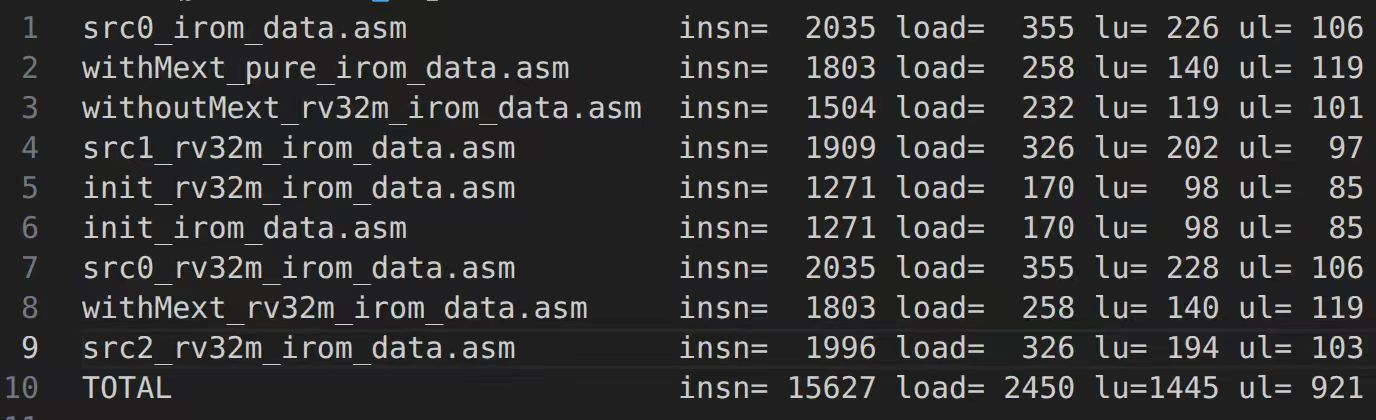
\includegraphics[width=\textwidth,height=0.68\textheight,keepaspectratio]{load-use_use-load_cmp.jpg}
  \caption{load-use 和 use-load 发生频率对比分析}
  \label{fig:lu_ul_cmp}
\end{figure}

为了降低“AGU 提前计算”的设计对主频带来的影响，ISU为 AGU 配备了专用的提前比较与独热码旁路网络。AGU 在 ISS 阶段计算 \id{rs1+imm}，对紧邻生产者（EX1）无法直接旁路的情况插入一个周期的 interlock，随后从 EX2 或更后级选择正确基址。

\subparagraph{执行单元 EXU}

EXU 为四级流水线单元，分为 EX1--EX4 四个流水线阶段。

EX1 完成 ALU、运算，以及向LSU、乘除法器发送相应请求；
EX2 从 LSU 获取 load-word 访存结果；
EX3 从 LSU 获取 load-half/byte 访存结果，并交由 BRU 完成 Branch 计算，寄存 control-hazard 信号，产生控制冒险判断结果；
EX4 向 LSU 发送 store data 写数据，并向前后端广播control-hazard，进行流水线寄存器冲刷。

ALU 支持 32 位加减、按位逻辑、逻辑/算术移位和有符号/无符号比较。
BRU 支持六类条件分支及 JAL/JALR，产生真实 next PC。JALR 的最低位清零，保证目标地址符合规范。

\subparagraph{乘除法单元}

乘法器使用 Vivado Multiplier IP 核，经过 4 周期固定延迟，计算得出 64 bit 乘积，由 WBU 根据 MUL、MULH、MULHSU、MULHU 指令decode生成的控制信号，选择低 32 bit或高 32 bit。当前配置乘法延迟为 4 周期。

除法器使用 Vivado Divider IP 核，经过固定周期延迟，支持有符号和无符号商/余数运算。为维持顺序提交，较新的 DIV/REM 在已有除法在途时停留于 ISS；当除法到达 WB 但结果尚未完成时，全流水线冻结。

\subparagraph{浮点运算单元}

由于 IP 核提供的乘除、乘加、加减单元均只有 RNE 的舍入模式，而 F 扩展要求有 5 种
舍入模块，同时 IP 核缺少 NX 异常输出，因此本处理器的浮点运算单元均不使用 IP 核而
独立实现，目前除乘除、乘加单元其它运算单元已经实现。由于尚未完整实现 FPU 且目前的
测试程序暂时不对 F 扩展进行测试，因此没有在代码配置中开启 F 扩展的使用。

\subparagraph{CSR 与异常处理}

CSR 单元通过掩码选择目标寄存器，并对 RW、RS、RC 三类命令执行覆盖、置位和清位。
立即数 CSR 指令将 zimm 零扩展后复用同一写数据通路。当前基础 CSR 如表
~\ref{tab:csr} 所示。

\begin{table}[H]
  \centering
  \caption{机器模式 CSR 实现}
  \label{tab:csr}
  \begin{adjustbox}{max width=\linewidth}
\begin{tabular}{cccP{7.0cm}}
    \toprule
    CSR & 地址 & 复位值 & 用途 \\
    \midrule
    \id{mstatus} & \id{0x300} & \id{0x00001800} & 保存 MIE/MPIE 等机器模式状态 \\
    \id{mtvec} & \id{0x305} & 0 & Direct 模式异常入口地址 \\
    \id{mscratch} & \id{0x340} & 0 & 当前配置可选并已使能 \\
    \id{mepc} & \id{0x341} & 0 & 保存触发 ECALL 指令的 PC \\
    \id{mcause} & \id{0x342} & 0 & ECALL from M-mode 写入 11 \\
    \bottomrule
  \end{tabular}
\end{adjustbox}
\end{table}

执行 ECALL 时，CSR 单元将当前指令 PC 写入 \id{mepc}，将 11 写入
\id{mcause}，把原 MIE 保存至 MPIE 并清零 MIE，随后 PC 重定向至
\id{mtvec}。执行 MRET 时，PC 重定向至 \id{mepc}，MIE 恢复为 MPIE，MPIE
置 1。该流程与区域赛给出的最小 trap 测试范围一致。

\subparagraph{访存单元 LSU}

LSU 接收已由 ISU/AGU 计算的地址、写数据、访问宽度和读写属性。对 Store 指令，
PERIP 写使能只在请求真正握手时产生；对 Load 指令，LSU 将返回数据按 byte、half、
word 截取，并依照 LB/LH 或 LBU/LHU 做符号/零扩展。若下游暂停，返回结果通过保持
寄存器保存，避免存储器返回数据丢失。

在 LS4 阶段 LSU 才会将数据写回内存或外设，这可以延长数据准备的时间，减少因等待数据
计算完成而停顿的时间，如 mul 指令要在 EX4 阶段才可以计算出，如果下一条指令要将 mul 指令
的计算结果写入内存或外设，则 LSU 可通过数据前递将结果提供给 LS4，消除停顿。

而将数据写回内存或外设的时机放在 LS4 阶段会与 LS1、LS2 可能的读指令产生结构冒险，这又会
产生新的停顿。对于写外设和读操作，由于读写外设的顺序一般不可改变，所以优先保证写操作
进行而将读指令进行停顿；对于写内存和读操作，则会先将要写入内存的数据写入 store buffer，
而不让写指令占用总线的使用，优先进行读操作，写入 store buffer 的数据会在总线空闲时再后台
自动写入内存。

\begin{figure}[htbp]
  \centering
  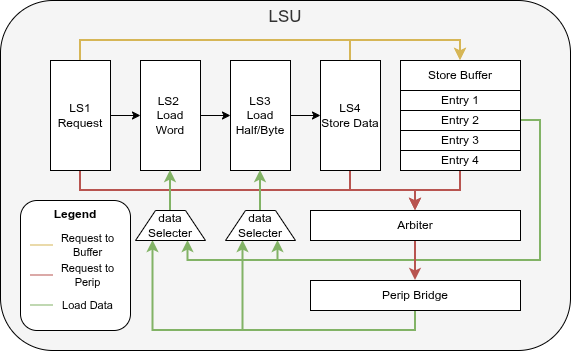
\includegraphics[width=\textwidth,height=0.68\textheight,keepaspectratio]{lsu architecture.png}
  \caption{四级流水 LSU 架构图}
  \label{fig:lsu architecture}
\end{figure}

数据写入 Store Buffer 时会先判断 Store Buffer 中有没有相同写入地址且有效的条目，如果有
则将新的写入数据合并进旧的条目中，如果没有则写入到由 sb\_wr\_ptr 维护的 Buffer 队列末尾。
若 sb\_count 为 4 则表示 Store Buffer 已满，需要停顿让 Store Buffer 有空间来接收新数据。

在从 Store Buffer 中读数据时，会先判断读地址是否与 Store Buffer 中有效条目中的一条相同，
若有则表示命中，会将从 Buffer 中读出的数据与从 Bram 读出的数据合并然后返回。

\begin{figure}[htbp]
  \centering
  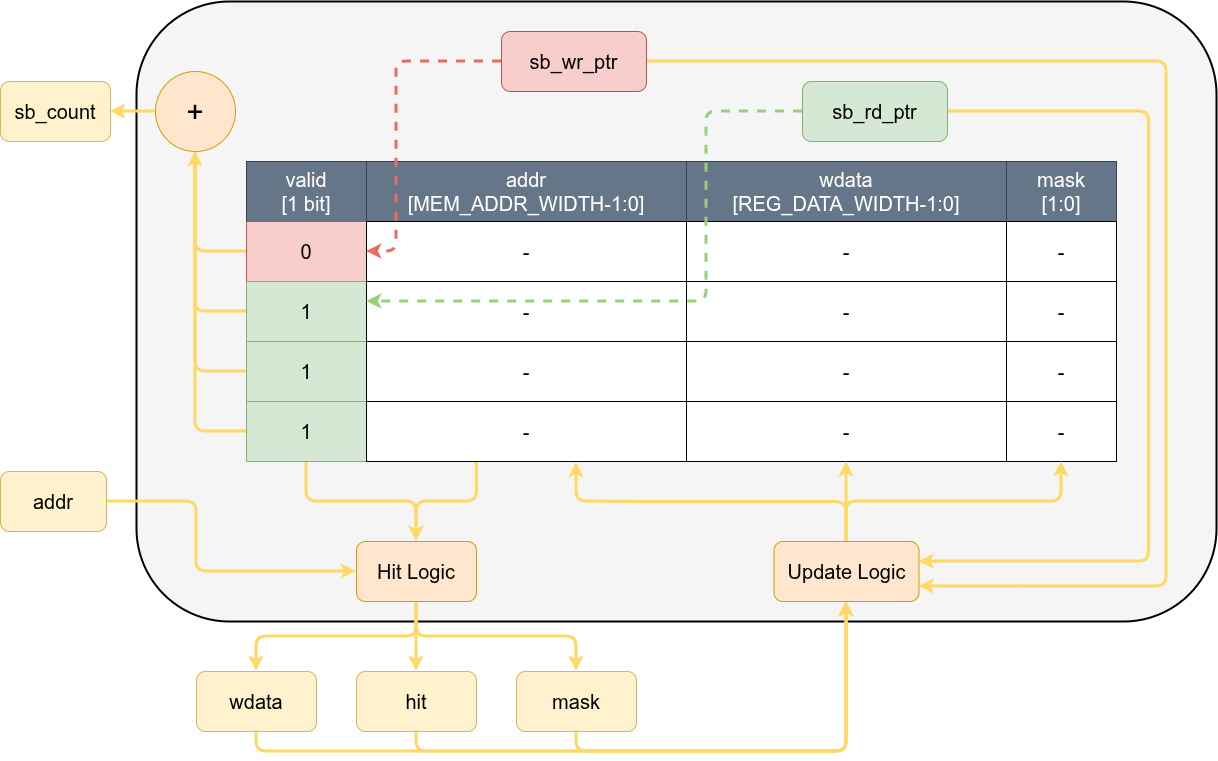
\includegraphics[width=\textwidth,height=0.68\textheight,keepaspectratio]{store_buffer_architecture.png}
  \caption{Store Buffer 结构示意图}
  \label{fig:store_buffer_architecture}
\end{figure}

\subparagraph{写回单元 WBU}

WBU 是顺序提交点，选择普通执行结果、乘法结果或除法结果写回通用寄存器堆。
除法未完成时，会阻塞 WB 阶段，以确保顺序提交。
\id{x0} 的恒零约束由寄存器堆实现。仿真环境以 WBU 的有效提交作为 guest 指令计数
依据，并在该处获得访存和环境指令信息。

\paragraph{冒险处理}

\subparagraph{数据冒险与旁路网络}
\label{subsec:bypass}

本设计将数据冒险主要分开为回答三个问题：\textbf{生产者什么时候能生产出可旁路的数据；消费者什么时候需要生产者的数据；被旁路的数据在哪里。}

为\textbf{解决“生产者什么时候能生产出可旁路的数据；消费者什么时候需要生产者的数据”两个问题}，本设计在 IDU 阶段，根据不同的指令类型，给出了各个指令的\textbf{生产时机}和\textbf{消费时机}。
生产时机由 5 bit 的 \id{PROD_ABS} 温度计码表示。从低位到高位依次对应 EX1、EX2、EX3、
EX4 和 WB 检查点；某一位为 1 表示结果到该检查点仍未就绪，为 0 表示此时已经可以旁路。
因此，连续的低位 1 越多，代表生产者产生结果越晚。当前 IDU 实际使用的生产时机编码如
表~\ref{tab:idu-produce-time} 所示。

\begin{table}[H]
  \centering
  \caption{IDU 生产时机编码}
  \label{tab:idu-produce-time}
  \begin{tabularx}{0.96\textwidth}{P{4.1cm}C{1.8cm}C{1.9cm}X}
    \toprule
    编码 & 温度计码 & 结果可旁路时机 & 对应的指令 \\
    \midrule
    \code{PROD_ABS_EX1} & \code{00000} & EX1末期 & 普通整数运算、移位和比较指令，\id{JAL/JALR}、CSR 指令、\id{AUIPC/LUI} \\
    \code{PROD_ABS_EX2} & \code{00001} & EX2末期 & \id{LW} \\
    \code{PROD_ABS_EX3} & \code{00011} & EX3末期 & \id{LB/LH/LBU/LHU} \\
    \code{PROD_ABS_EX4} & \code{00111} & EX4末期 & 暂无生产者 \\
    \code{PROD_ABS_WB_EARLY} & \code{01111} & WB早期 & \id{MUL/MULH/MULHSU/MULHU} \\
    \code{PROD_ABS_WB_LATE} & \code{11111} & WB完成 & \id{DIV/DIVU/REM/REMU} \\
    \bottomrule
  \end{tabularx}
\end{table}

其中，\id{PROD_ABS_EX1}，与\id{CONS_EX4}，等效为立刻可以生产/最晚才需要消费，故不生产数据/不消费数据的指令，统一被编码为\id{PROD_ABS_EX1}，与\id{CONS_EX4}。

当前 IDU 使用的消费时机编码如表~\ref{tab:idu-consume-time} 所示。

\begin{table}[H]
  \centering
  \caption{IDU 消费时机编码}
  \label{tab:idu-consume-time}
  \begin{tabularx}{0.96\textwidth}{P{3.7cm}C{1.8cm}C{2.2cm}X}
    \toprule
    编码 & 温度计码 & 消费时机 & 对应的指令 \\
    \midrule
    \code{CONS_ISS_EARLY} & \code{11111} & ISS 早期 & Load/Store 类指令的地址 base \id{rs1} \\
    \code{CONS_ISS_LATE} & \code{11110} & ISS 末期 & 基本 ALU 运算  \\
    \code{CONS_EX1} & \code{11100} & EX1 & 暂无消费者 \\
    \code{CONS_EX2} & \code{11000} & EX2 & branch 指令 \\
    \code{CONS_EX3} & \code{10000} & EX3 & CSR 指令、store 指令 \\
    \code{CONS_EX4} & \code{00000} & EX4 & 暂无消费者 \\
    \bottomrule
  \end{tabularx}
\end{table}

IDU 给出的 \id{PROD_ABS_*} 以生产者自身的流水过程为绝对时间坐标，而相关判断发生时，
消费者正位于 ISS，生产者可能已经处于 EX1 至 WB 中的任意一级。因此，ISU 需要结合
生产者的当前位置，将绝对未就绪温度计码平移成“从当前消费者出发还要等待多久”的相对
未就绪温度计码。本文将平移后的六种取值命名为 \id{PROD_REL_*}，如
表~\ref{tab:producer-relative-time} 所示。

\begin{table}[H]
  \centering
  \caption{生产者相对未就绪温度计码}
  \label{tab:producer-relative-time}
  \begin{tabularx}{0.86\textwidth}{P{4.5cm}C{2.0cm}X}
    \toprule
    编码 & 温度计码 & 从当前消费者观察的结果可用时机 \\
    \midrule
    \code{PROD_REL_ISS_EARLY} & \code{00000} & 当前 ISS 早期已经可用 \\
    \code{PROD_REL_ISS_LATE}  & \code{00001} & 当前 ISS 末期可用 \\
    \code{PROD_REL_EX1}       & \code{00011} & 消费者进入 EX1 时可用 \\
    \code{PROD_REL_EX2}       & \code{00111} & 消费者进入 EX2 时可用 \\
    \code{PROD_REL_EX3}       & \code{01111} & 消费者进入 EX3 时可用 \\
    \code{PROD_REL_EX4}       & \code{11111} & 消费者进入 EX4 时可用 \\
    \bottomrule
  \end{tabularx}
\end{table}

为\textbf{解决“被旁路的数据在哪里”的问题}，本设计在 ISU 阶段组合地生成数据冒险发生位置 \id{where} 信号。具体生成过程如下。对于 \id{rs1} 和 \id{rs2}，ISU 分别将源寄存器编号与 EX1、EX2、
EX3、EX4、WB 各级携带的目的寄存器编号比较。某一级的匹配条件可以表示为
\code{match_s = rs_ren && stage_valid && rd_wen && (rd != x0) && (rs == rd)}：只有消费者确实
读取该源寄存器、该级指令有效且会写非零目的寄存器时，才认为存在 RAW 相关。各级匹配
结果按照表~\ref{tab:where-layout} 的布局组成 5 bit 的 \id{where}。\id{rs1} 和
\id{rs2} 各自维护一份 \id{where}。

\begin{table}[H]
  \centering
  \caption{where 相关位置向量的位布局}
  \label{tab:where-layout}
  \begin{tabularx}{0.76\textwidth}{C{2.0cm}C{1.5cm}X}
    \toprule
    位 & 对应位置 & 置 1 条件 \\
    \midrule
    \code{where[4]} & EX1 & 源寄存器与 EX1 的有效目的寄存器匹配 \\
    \code{where[3]} & EX2 & 源寄存器与 EX2 的有效目的寄存器匹配 \\
    \code{where[2]} & EX3 & 源寄存器与 EX3 的有效目的寄存器匹配 \\
    \code{where[1]} & EX4 & 源寄存器与 EX4 的有效目的寄存器匹配 \\
    \code{where[0]} & WB  & 源寄存器与 WB 的有效目的寄存器匹配 \\
    \bottomrule
  \end{tabularx}
\end{table}

如果多条在途指令连续写同一个寄存器，
其中可以同时有多个 bit 为 1。获得 \id{where} 后，设绝对生产码为
\id{PROD_ABS[4:0]}，从高位到低位依次对应 WB、EX4、EX3、EX2、EX1，则 \id{ISU}
针对生产者的五种可能位置生成
表~\ref{tab:producer-relative-shift} 中的候选码。随后，\id{PROD_REL} 使用
\id{where} 选通相应候选码并按位或，得到最终的 \id{PROD_REL}。

\begin{table}[H]
  \centering
  \caption{绝对生产码到相对未就绪码的平移}
  \label{tab:producer-relative-shift}
  \begin{tabularx}{0.94\textwidth}{C{2.2cm}P{6.3cm}X}
    \toprule
    生产者位置 & 候选相对码的生成方式 & 含义 \\
    \midrule
    EX1 & \code{[PROD_ABS[3:0], 1'b1]} & 末位补 1，表示 EX1 结果无法旁路到 ISS 早期 \\
    EX2 & \code{[1'b0, PROD_ABS[3:0]]} & 相对 EX1 情况前进一级 \\
    EX3 & \code{[2'b00, PROD_ABS[3:1]]} & 移去两个已经经过的检查点 \\
    EX4 & \code{[3'b000, PROD_ABS[3:2]]} & 仅保留尚未经过的检查点 \\
    WB  & \code{[4'b0000, PROD_ABS[4]]} & 普通结果已经就绪；除法未完成时保留末位未就绪标志 \\
    \bottomrule
  \end{tabularx}
\end{table}

生产者每向后推进一级，候选相对码便右移一位，移去一个已经经过的检查点，并在高位补 0。例如，普通 ALU 指令的绝对码为
\id{00000}，当它位于 EX1 时得到 \id{00001}，即 \id{PROD_REL_ISS_LATE}；该值与后继
普通指令的 \id{CONS_ISS_LATE}（\id{11110}）按位相与为 0，因此可以直接旁路。\id{LW}
的绝对码为 \id{00001}，当它位于 EX1 时得到 \id{00011}，即 \id{PROD_REL_EX1}；与
\id{CONS_ISS_LATE} 按位相与的结果非零，因此后继指令停顿一周期。下一周期 \id{LW}
进入 EX2，相对码变为 \id{00001}，此时即可旁路。类似地，AGU 基址使用
\id{CONS_ISS_EARLY}，即使紧邻的普通 ALU 生产者已经得到 \id{PROD_REL_ISS_LATE}，两者
按位相与仍非零，所以互锁逻辑会准确插入一个周期停顿。

互锁判断与旁路选择共用同一份 \id{where}。ISU 将消费者的 \id{CONS_*} 与
\id{PROD_REL_*} 按位相与；结果非零表示生产者无法赶上消费时机，需要触发
\id{interlock}。与此同时，各级生产者根据自身绝对生产码生成 \id{bypass_mask}，其位布局
与 \id{where} 完全相同，判断方式如表~\ref{tab:ready-mask} 所示。

\begin{table}[H]
  \centering
  \caption{旁路数据就绪掩码}
  \label{tab:ready-mask}
  \begin{tabularx}{0.86\textwidth}{C{1.5cm}C{2.0cm}X}
    \toprule
    位置 & 掩码位 & 置 1 条件 \\
    \midrule
    EX1 & \code{bypass[4]} & EX1 有效、写寄存器，且 \id{PROD_ABS[0]} 为 0 \\
    EX2 & \code{bypass[3]} & EX2 有效、写寄存器，且 \id{PROD_ABS[1]} 为 0 \\
    EX3 & \code{bypass[2]} & EX3 有效、写寄存器，且 \id{PROD_ABS[2]} 为 0 \\
    EX4 & \code{bypass[1]} & EX4 有效、写寄存器，且 \id{PROD_ABS[3]} 为 0 \\
    WB  & \code{bypass[0]} & WB 写回结果有效且写寄存器 \\
    \bottomrule
  \end{tabularx}
\end{table}

\Needspace{7\baselineskip}
将相关位置与就绪掩码按位相与，即得到当前真正可用的旁路源。如果没有任何 bit 置 1，旁路选择为
\id{FWD_NONE}；否则按照 EX1、EX2、EX3、EX4、WB 的顺序进行优先选择，生成独热的
\id{FWD_EX1} 至 \id{FWD_WB}。由于处理器顺序单发射，位置越靠近 EX1 的生产者越年轻，
这一优先级可以保证多条在途指令写同一寄存器时总是选择最新值。

旁路数据通路分两次完成操作数修正。第一次位于 ISS：\id{ISU} 使用独热选择信号，
在寄存器堆读数以及 EX1、EX2、EX3、EX4、WB 五路结果之间选择，得到
\id{rs1_val_iss} 和 \id{rs2_val_iss}。选择 \id{FWD_NONE} 时保留寄存器堆读数，否则用
对应流水级的结果覆盖。

消费者进入 EX1 时，\id{advance_where} 将尚未解决的相关位置随生产者一起向后移动一级，
形成 \id{where_ex1}。已经在 ISS 取得的生产者以及所有更老的匹配项会被清除；尚未就绪的
更年轻生产者则继续保留。EX1 使用新的 \id{where_ex1} 与当前 \id{bypass_mask} 再次计算
旁路源：若更年轻的结果此时变为可用，\id{ISU} 用该结果覆盖 ISS 已经取得的值；
否则保留 \id{rs1_val_iss} 和 \id{rs2_val_iss}。这一两级旁路结构既能尽早取得现有结果，
又能避免较老的结果覆盖稍后才就绪的年轻结果。

\subparagraph{控制冒险}

EX3 BRU计算完成分支跳转结果后，解析控制流指令，并将预测 PC、预测方向、真实 PC 和真实方向送入 HZU。预测错误时，
经一拍寄存后，HZU 在 EX4 阶段，产生重定向地址并冲刷前端至 EX3 之前的错误路径指令。IFU 同拍禁止新取指并清除
响应有效位与预测暂存，同时屏蔽相应流水线寄存器的输出，使旧路径的在途 IROM 数据不会再作为有效
事务进入流水线。

\subparagraph{结构冒险}

数据在 LS4 阶段通过总线写回，而在 LS1、LS2 阶段可能会有 load 指令通过总线读数据，
这会因总线接口被同时访问产生结构冒险。解决方式为优先进行写操作，而将需要读总线的指
令暂停，这样可以保证外设原来的读写顺序。同时为了减少因结构冒险而产生的停顿，在写入 bram
时会先不访问总线而将数据先写入到 store buffer 中，这样可以减少总线的占用，为读操作留出
总线的使用权，减少停顿。存入 store buffer 的数据会在总线空闲的时候写入 bram，且
在 store buffer 已满并有 load 指令和写入 bram 的指令正在执行时仍会产生结构冒险并停顿。

\paragraph{OV5640 摄像头视频通路}

  OV5640 通过 DVP 8 位接口输出图像。
FPGA 先通过 SCCB 总线完成传感器上电时序和寄存器配置，将输出格式设置为 RGB565；DVP 接收模块对 8 位字节流做确定性配对，恢复 16 位像素，
并在 HREF 低电平期间复位字节相位，避免行长变化或毛刺造成奇偶字节错位。像素处理时钟由 DVP 时钟二分频得到，
数据经过三级流水后送入后续处理，以匹配同步存储器和跨时钟域接口的时序。

  视频通路分为缩略图和整帧两条支路，如图~\ref{fig:ov5640-video-path}所示。
缩略图支路在 1280$\times$720 有效画面中取中心 640$\times$640 窗口，
按 20$\times$20 像素单元做 4:1 盒式滤波，降采样为 32$\times$32 RGB565 图像，
并通过双 bank 和异步 FIFO 写入片上 BRAM；SoC 通过 MMIO 窗口读取当前帧，
供 miniTensor 手势识别使用。整帧支路保留完整 1280$\times$720 图像，经 DDR3 双缓冲后由 HDMI 以 720p30 输出，
用于实时预览和演示。


\begin{figure}[htbp]
  \centering
  % 适当放大：允许图宽略超正文宽度，居中放置。
  \makebox[\linewidth][c]{%
    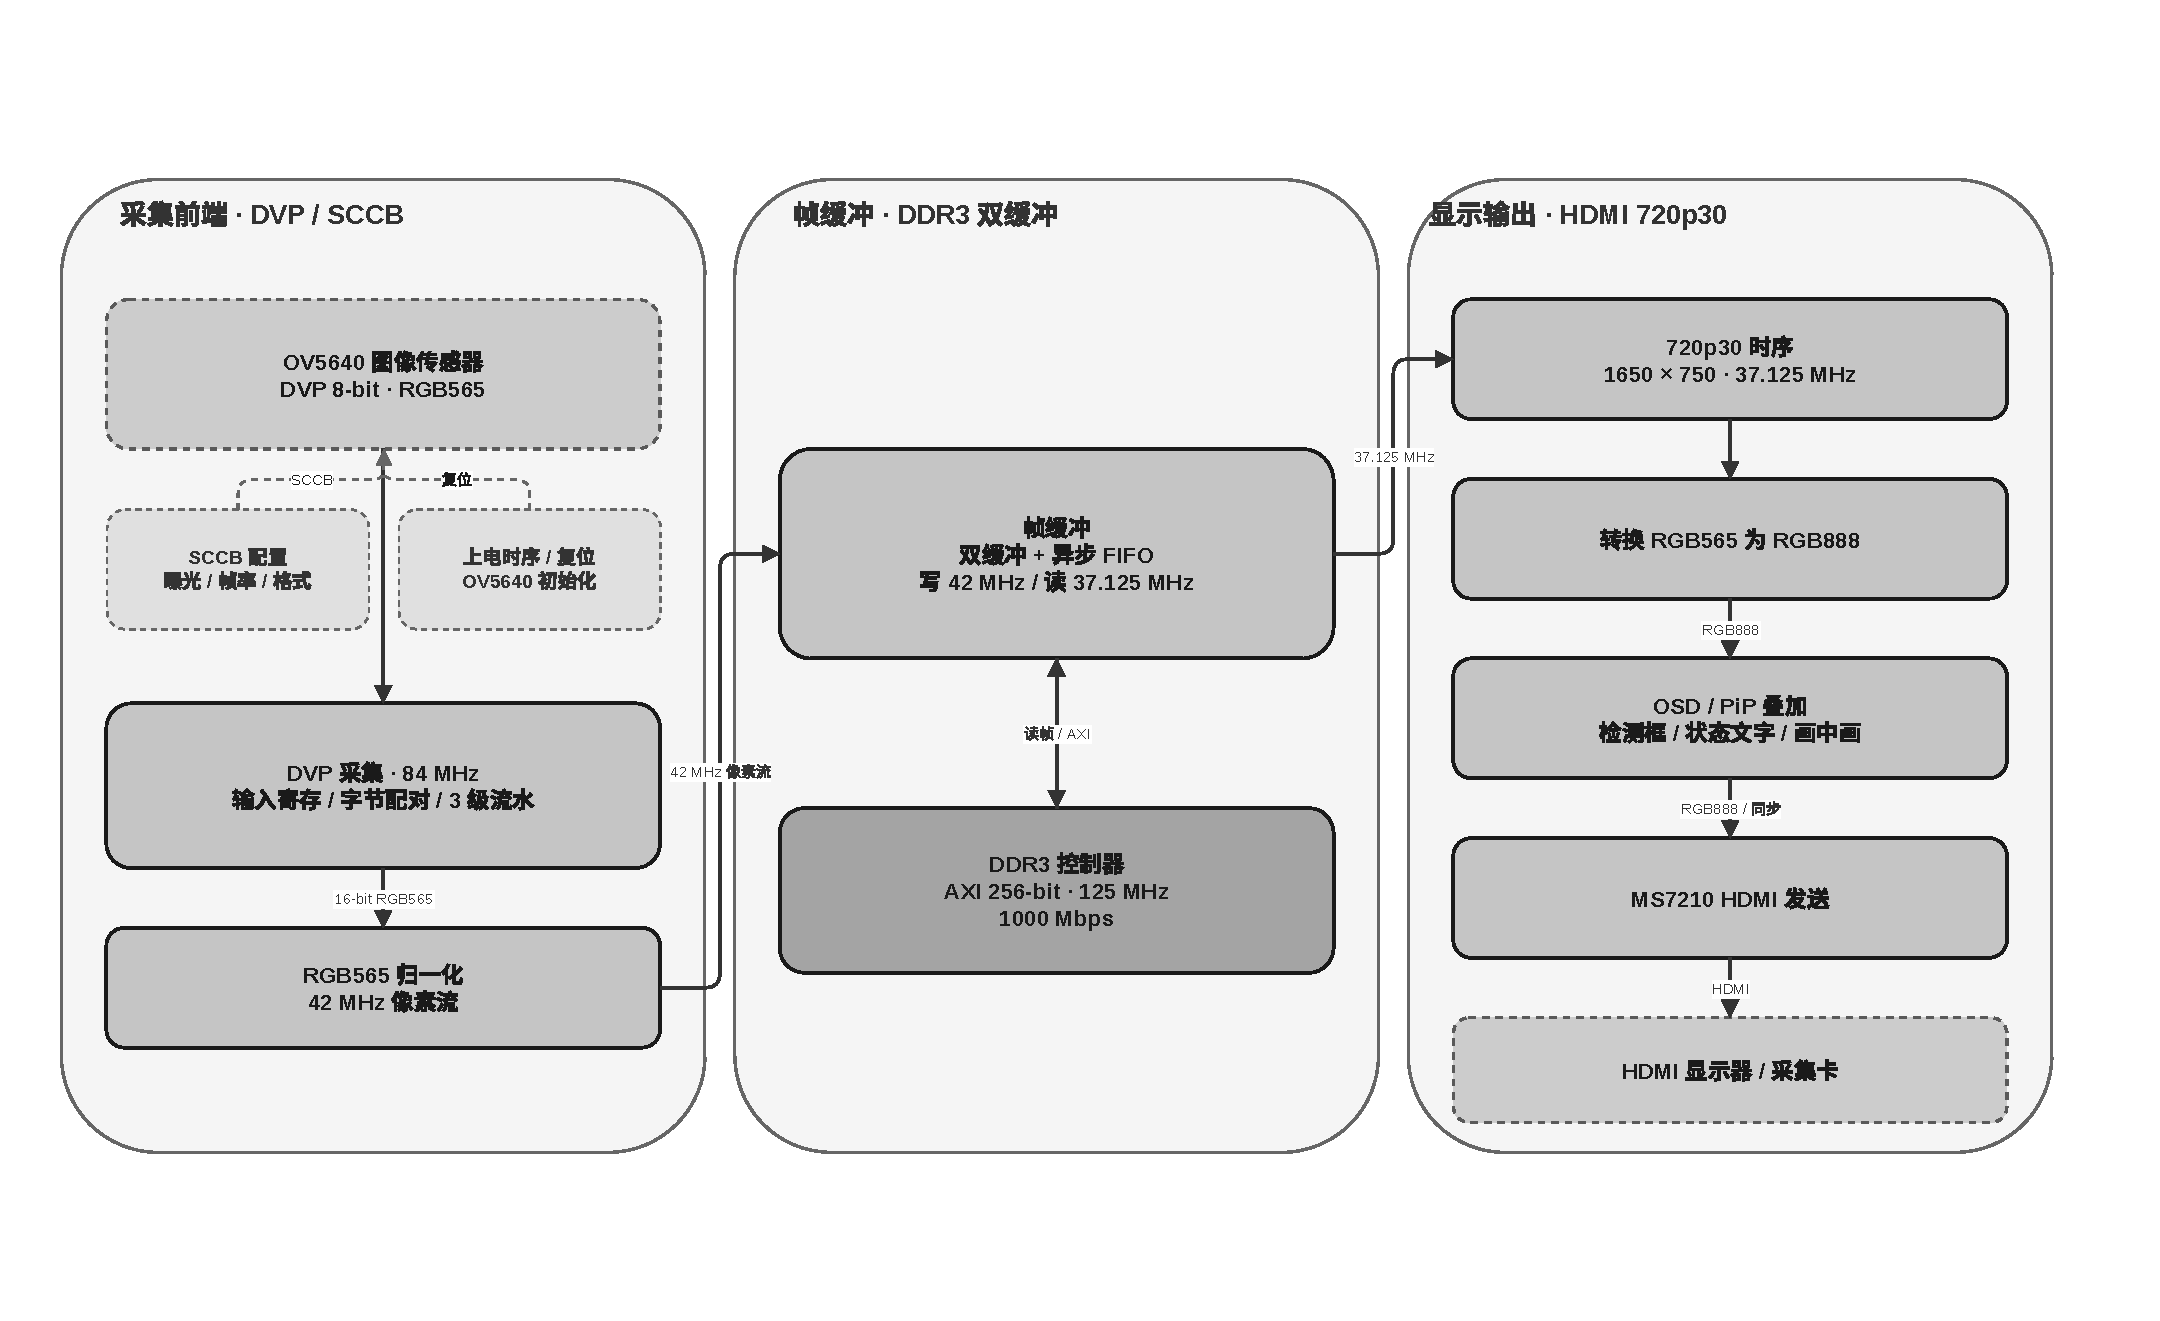
\includegraphics[width=1.10\linewidth,height=0.95\textheight,keepaspectratio]{figures/module10_ov5640_video.drawio.pdf}%
  }
  \caption{OV5640 摄像头视频通路}
  \label{fig:ov5640-video-path}
\end{figure}

\subsection{软件系统介绍}
\subsubsection{软件整体介绍}
软件包括目标端裸机运行时和测试程序，以及主机端 Verilator 仿真框架、参考模型、波形和日志工具。
演示应用还包括运行在主机浏览器中的 Web 控制器，它通过串口接收板端手势识别结果，驱动 HTML 演示页面完成场景切换与视觉反馈。
目标端程序完成指令与算法计算，主机端负责镜像加载、时钟复位、行为比对、性能计数和 IO 模拟，两者通过 DPI-C 提交及分支事件连接。
\subsubsection{软件各模块介绍}
\paragraph{仿真平台}

现有验证平台使用 Verilator 将 Chisel 生成的 SystemVerilog 编译为 C++ 模型，C/C++
仿真框架负责镜像加载、时钟激励、存储器模型、日志、性能计数和波形输出。RTL 通过
DPI-C 将提交、访存和分支预测事件传给仿真框架；GTKWave 用于查看 Verilator 生成的
FST 波形。整个流程不依赖 FPGA 即可完成大规模程序运行和错误定位。

\paragraph{软件测试环境}

原测评报告记录的软件环境为 Ubuntu 24.04、Verilator 5.046、GTKWave 3.3.116、
GCC/G++ 13.3.0 和 RISC-V 交叉编译工具链。测试程序与裸机运行时环境共同编译，
链接至处理器能够访问的地址空间，再转换为仿真器或 Vivado IP 可以加载的镜像。

针对赛题的内存空间设计编写了专用的链接脚本以及入口函数，为编译程序提供最基本的
运行时环境。目标端地址空间与硬件采用相同的 IROM、DRAM 和外设映射，见第二部分的 SoC 地址空间。

\paragraph{硬件仿真环境}

硬件仿真环境由处理器模型、指令/数据存储器模型、时钟与复位激励、DPI-C 接口和参考
模型构成。测试开始时，仿真框架将程序镜像加载至存储器；处理器从复位入口开始执行；
每当 WBU 提交一条有效指令时，仿真框架更新 guest 指令数，并可将 PC、寄存器和访存
副作用与参考模型比较。出现不一致时立即停止运行并输出出错指令附近的状态。

BPU 采用独立的模块差分方式：取指侧比较预测方向和目标，更新侧把真实分支结果同时送入
RTL 和 C++ Bimodal 模型。发生重定向后已经无效的取指事件不参与预测质量统计。

\paragraph{测试程序}

仿真测试按用途分为四类：第一类是逐指令功能测试，用于覆盖 RV32I、RV32M、Zicsr
和异常返回；第二类是 CoreMark 等程序级测试，用于检查长程序稳定性并统计周期数和 IPC；
第三类是 BPU 模块差分测试，用于分别验证预测实现正确性与预测质量；
第四类是竞业达提供的 RV32I/RV32IM、CSR/trap 与性能镜像。

由于使用了 IP 核以及 FPGA io（student\_top 的 io 如图~\ref{fig:student_top}所示），为了确保仿真环境最大限度反映真实硬件情况，我们为仿真环境设计了 io 仿真，涵盖运行时间计算、数码管模拟、LED模拟三大功能。

\begin{figure}[htbp]
  \centering
  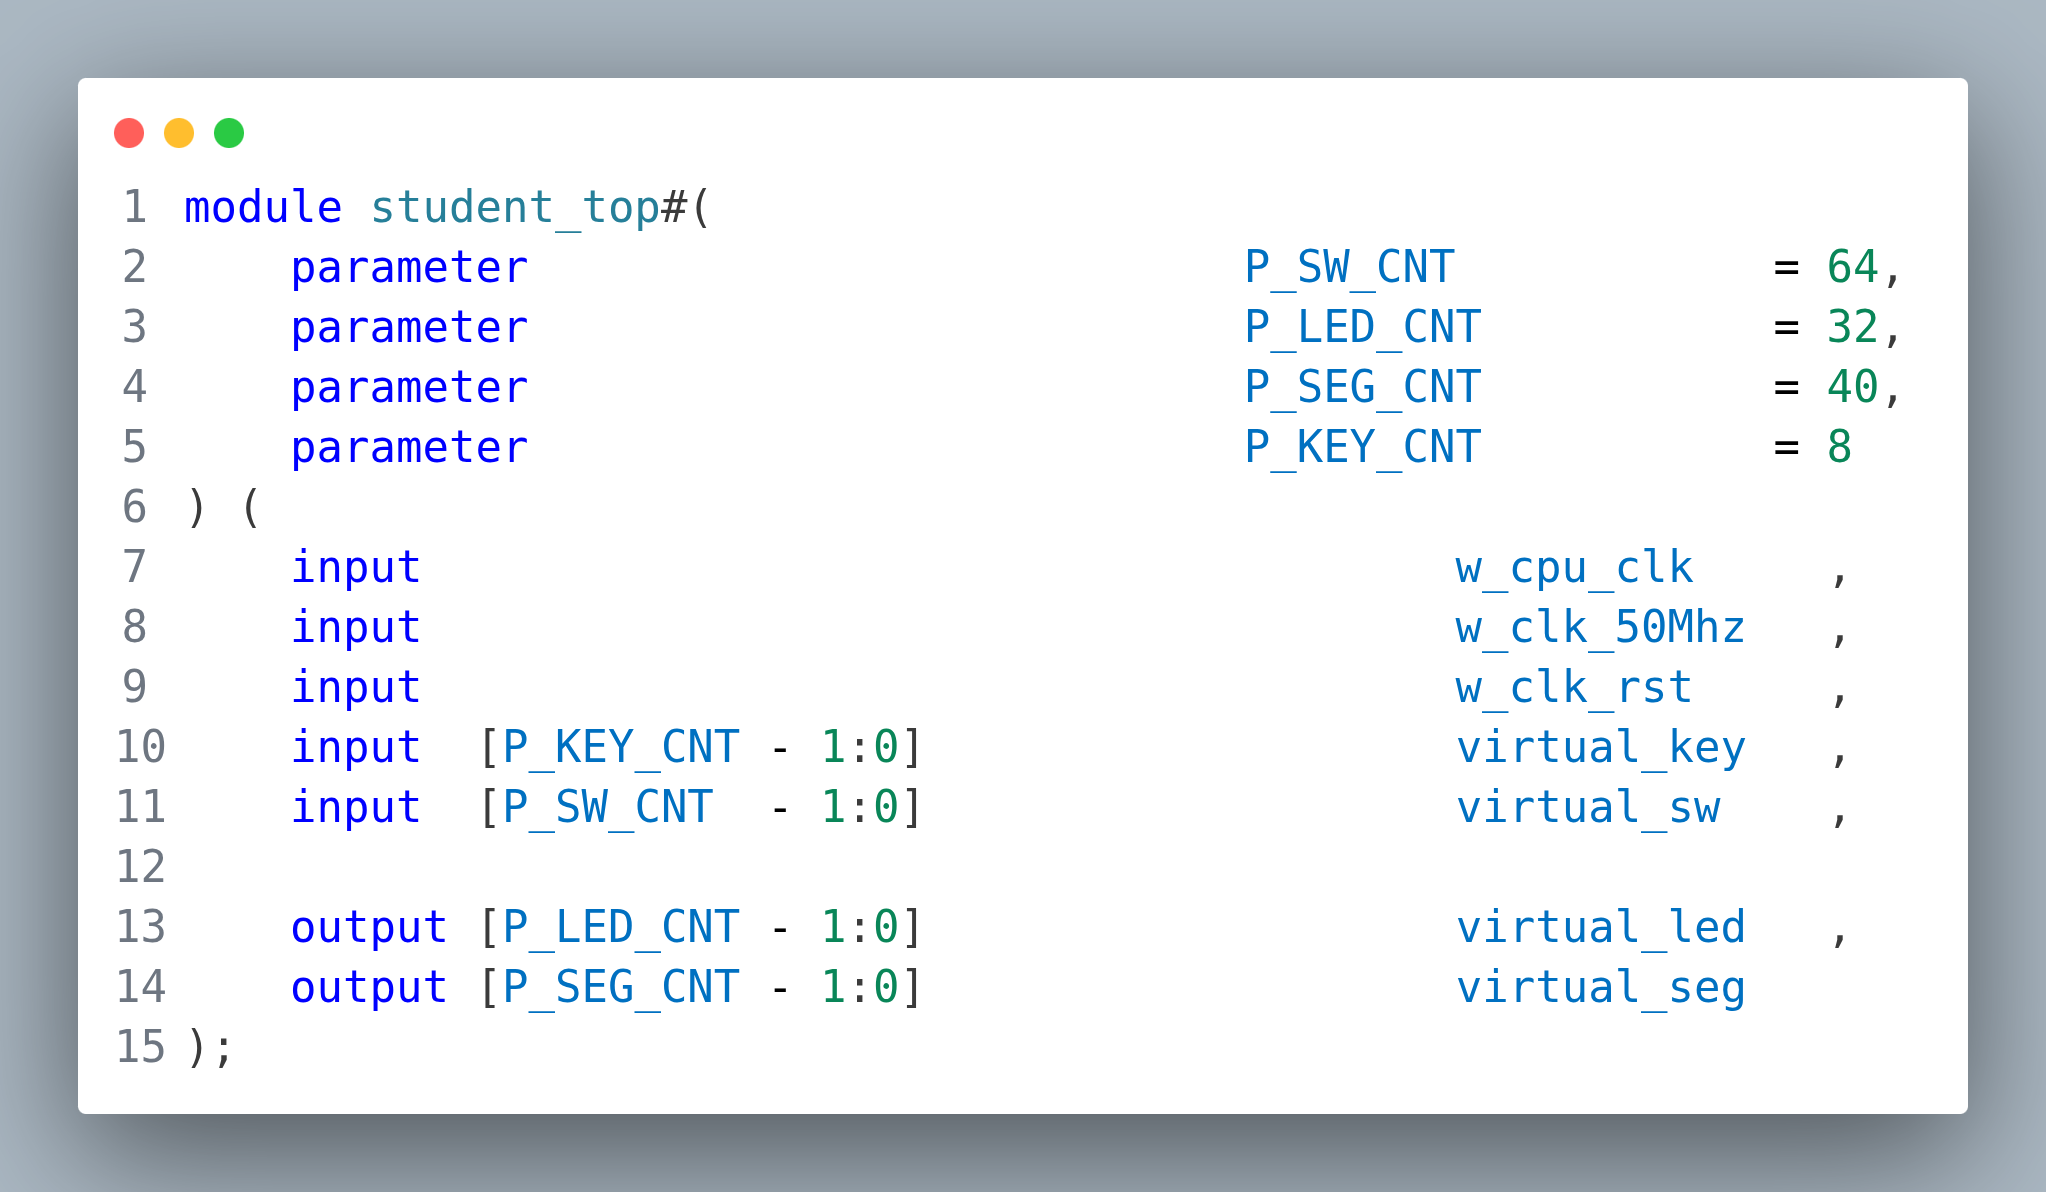
\includegraphics[width=0.90\linewidth,height=0.68\textheight,keepaspectratio]{student_top.png}
  \caption{student\_top.sv io}
  \label{fig:student_top}
\end{figure}

由图~\ref{fig:FPGA-sim-cmp}可见，仿真环境运行时间结果自洽（数码管和 log 处 execution time 均显示 8.637s），而且仿真环境 IO 输出也均与 FPGA IO 输出一致。可以认为仿真对 FPGA 有较好模拟作用。

\begin{figure}[htbp]
  \centering
  \begin{minipage}{0.48\linewidth}
    \centering
    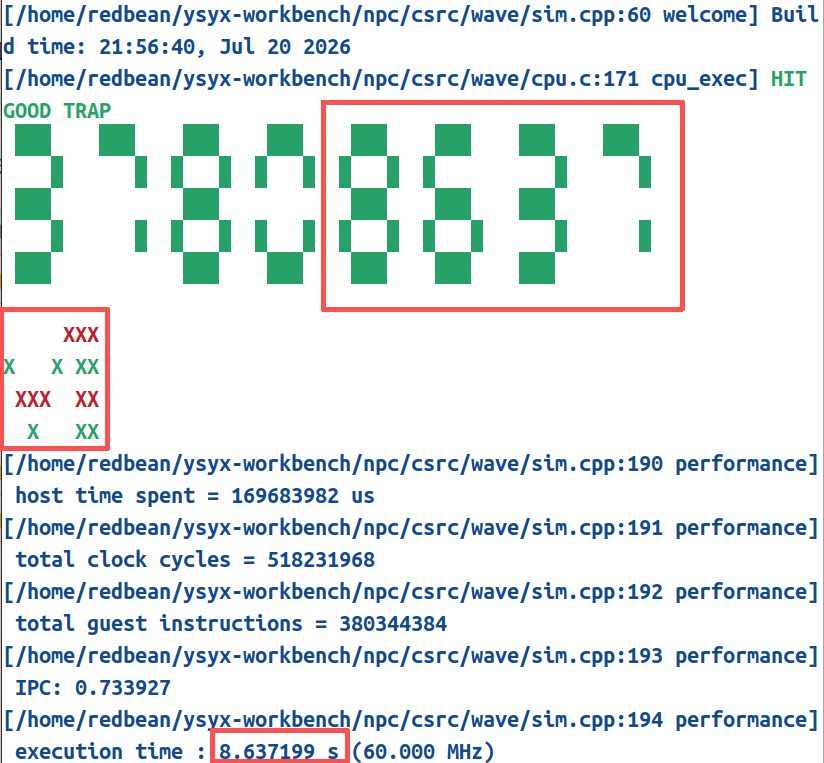
\includegraphics[width=\linewidth,height=0.68\textheight,keepaspectratio]{simulation_io.png}
    \caption*{(a) 仿真环境 60 MHz 运行情况}
  \end{minipage}
  \hfill
  \begin{minipage}{0.48\linewidth}
    \centering
    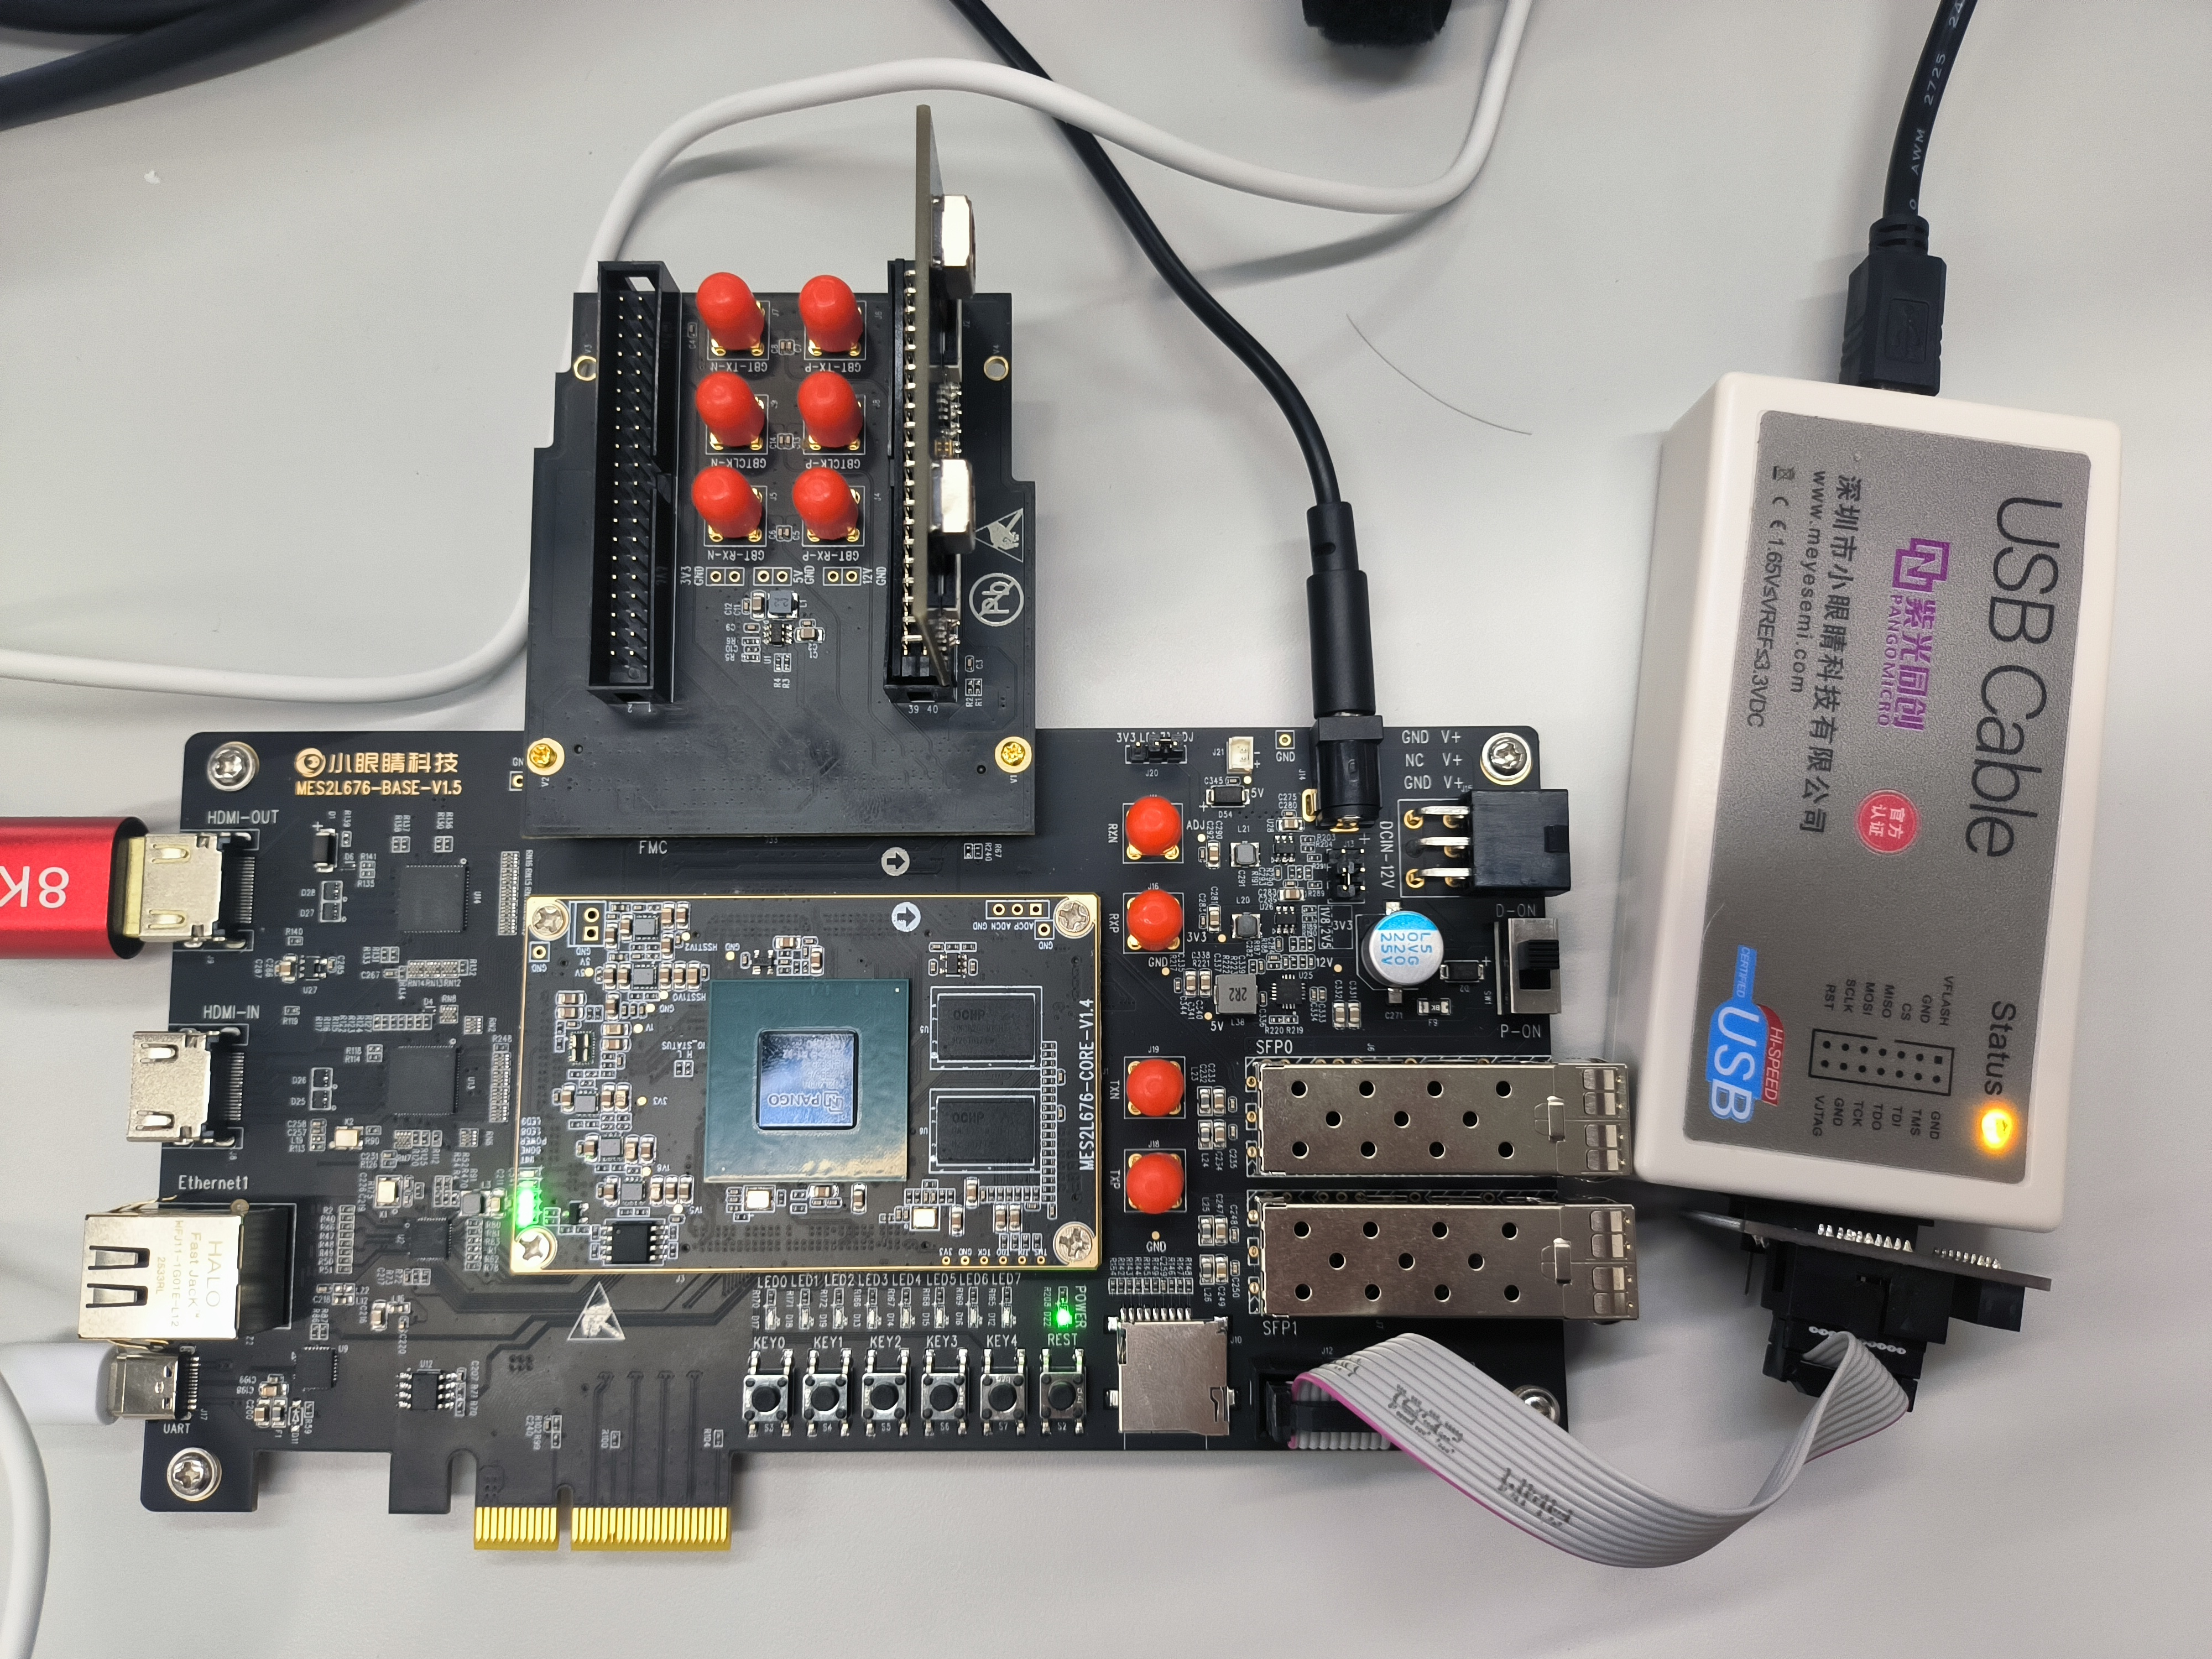
\includegraphics[width=\linewidth,height=0.68\textheight,keepaspectratio]{FPGA_io.png}
    \caption*{(b) FPGA 60 MHz 实际运行情况}
  \end{minipage}
  \par\medskip
  \caption{FPGA 和仿真环境对比图}
  \label{fig:FPGA-sim-cmp}
\end{figure}


\paragraph{工程模块组织}
以下保留当前工程文档中的模块目录，区分处理器 RTL、仿真框架、配置与工具。
\begin{lstlisting}[language={},numbers=none]
npc/
|-- scsrc/                 Chisel processor RTL
|   |-- Mundus.scala       Core top and pipeline control
|   |-- ifu/               BPU and IFU
|   |-- idu/               Instruction decoder
|   |-- isu/               Issue, register read, AGU, bypass
|   |-- exu/               ALU, BRU, CSR and EX1--EX4
|   |-- lsu/               Load/store unit
|   |-- mtu/, dvu/         Multiplier and divider
|   `-- wbu/               Commit and write-back
|-- vsrc/                  BlackBoxes, DPIC wrappers and FPGA IP
|-- csrc/                  Verilator runtime and reference checks
|-- configs/               Kconfig and generated configuration
|-- tools/                 Branch/cache analysis and helper tools
`-- build/                 Generated model and existing test logs
\end{lstlisting}

\begin{figure}[htbp]
\centering
\begin{tikzpicture}[node distance=5mm,>=Latex,
 flowprocess/.style={draw,align=center,text width=10cm,inner sep=4pt,font=\small}]
\node[flowprocess] (image) {编译、链接目标程序并生成 IROM/DRAM 镜像};
\node[flowprocess,below=of image] (load) {加载镜像，驱动复位、时钟及 IP 核模型};
\node[flowprocess,below=of load] (check) {采集 WBU、访存与分支事件，和参考模型比较};
\node[flowprocess,below=of check] (io) {更新 LED、数码管、计时器及性能统计};
\node[flowprocess,below=of io] (exit) {记录退出状态、日志、波形及预测质量报告};
\draw[->] (image)--(load);\draw[->] (load)--(check);
\draw[->] (check)--(io);\draw[->] (io)--(exit);
\end{tikzpicture}
\caption{主机仿真框架的运行与检查流程}
\label{fig:software-flow}
\end{figure}

\begin{table}[H]
\centering
\caption{软件模块的关键输入输出}
\begin{tabularx}{\linewidth}{@{}P{2.1cm}XX@{}}
\toprule
模块 & 关键输入 & 关键输出 \\
\midrule
运行时与镜像 & 链接布局、程序及初始数据 & 入口与 IROM/DRAM 镜像 \\
仿真驱动 & 镜像、复位、时钟 & 波形、日志与运行状态 \\
提交检查 & WBU 的 PC、寄存器和访存事件 & 一致性结果、指令计数 \\
BPU 差分 & 预测方向、目标、真实分支结果 & 模型匹配率与预测质量 \\
IO 模拟 & LED、SEG、计时控制 & 灯组、数码管和运行时间 \\
手势识别与网页控制 & 摄像头图像、串口指令 & 手势类别、页面状态、视觉效果 \\
\bottomrule
\end{tabularx}
\end{table}

\paragraph{手势识别与网页演示控制模块}

该模块把摄像头前的手势转换为网页演示控制指令，形成从手势识别、串口传输到网页状态机与视觉反馈的闭环。硬件端在 FPGA 上完成图像采集、固定取景区裁剪和 $32\times32$ 灰度归一化，由 miniTensor 上的轻量 INT8 卷积网络输出手势类别与置信度；固件通过连续多帧一致性和置信度门限抑制抖动，
再把确认后的手势转换为一行 ASCII 指令，经 115200 8N1 串口发送给上位机。
硬件端从图像采集到串口发送的通路如图~\ref{fig:gesture-hardware-path}所示。

\begin{figure}[htbp]
  \centering
  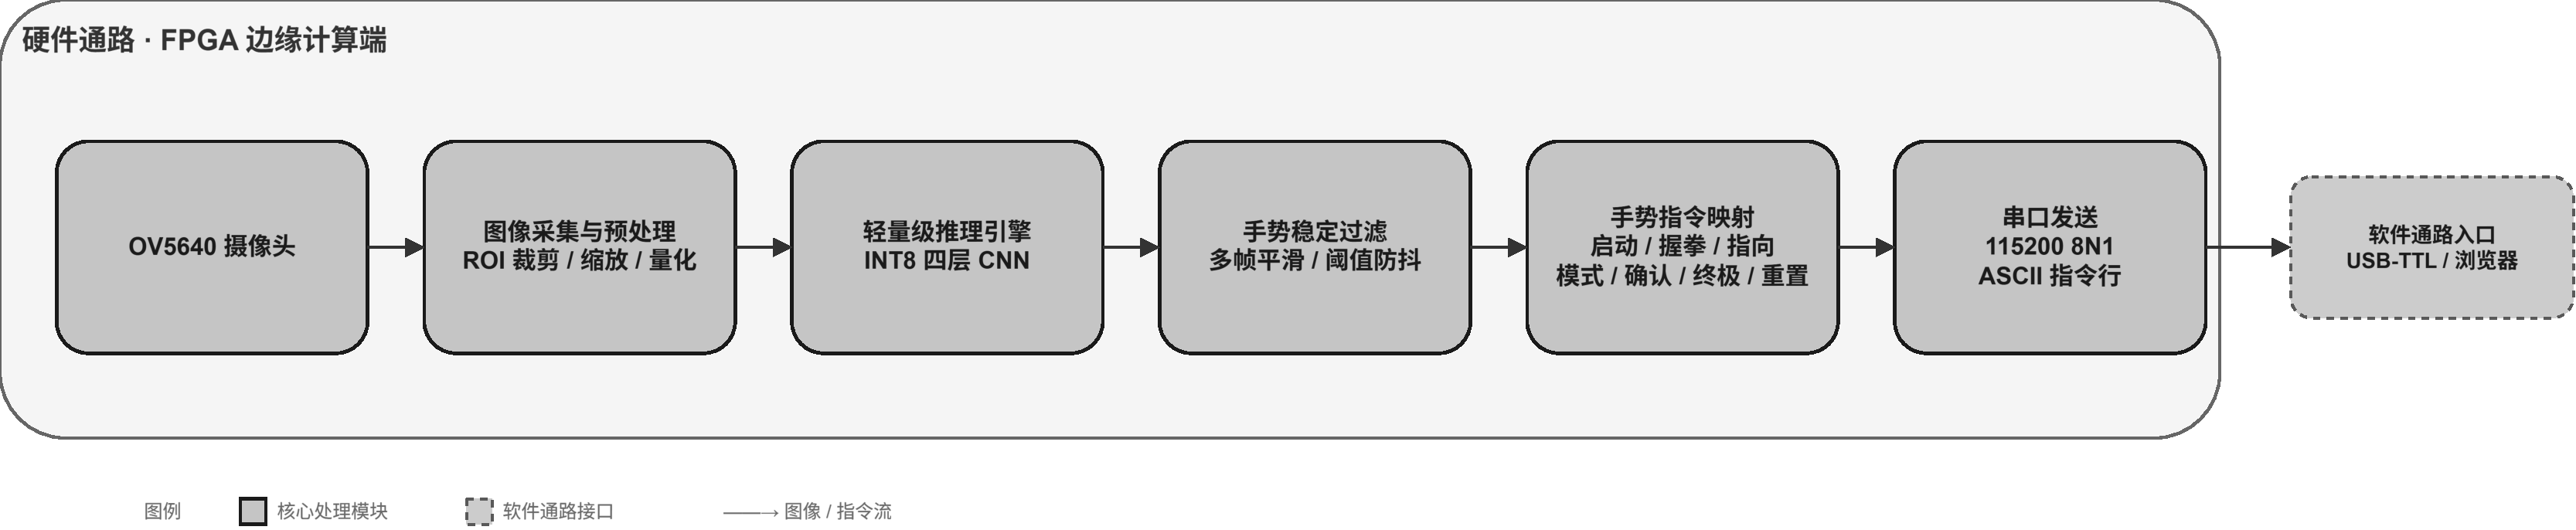
\includegraphics[width=\linewidth,height=0.42\textheight,keepaspectratio]{figures/gesture_web_hardware_path.pdf}
  \caption{手势识别与网页控制的硬件通路}
  \label{fig:gesture-hardware-path}
\end{figure}

上位机 Web 控制器基于 Web Serial API 和 Three.js 实现。串口字节流先经过行解析和指令解析，再由冷却/去重逻辑过滤重复手势，进入“基础状态 + 瞬时叠加层”的状态机；状态机只负责逻辑转移，效果层根据状态事件驱动粒子 Logo、全息球、激光扫描、能量波和 HUD 信息层等视觉元素。该分层使协议、状态逻辑和渲染相互独立，便于单元测试和现场调试；无硬件时可用键盘、调试面板或自动演示模式模拟指令。软件端从串口接入到全屏展示的通路如图~\ref{fig:gesture-software-path}所示。

\begin{figure}[htbp]
  \centering
  % 适当放大：允许图宽略超正文宽度，居中放置。
  \makebox[\linewidth][c]{%
    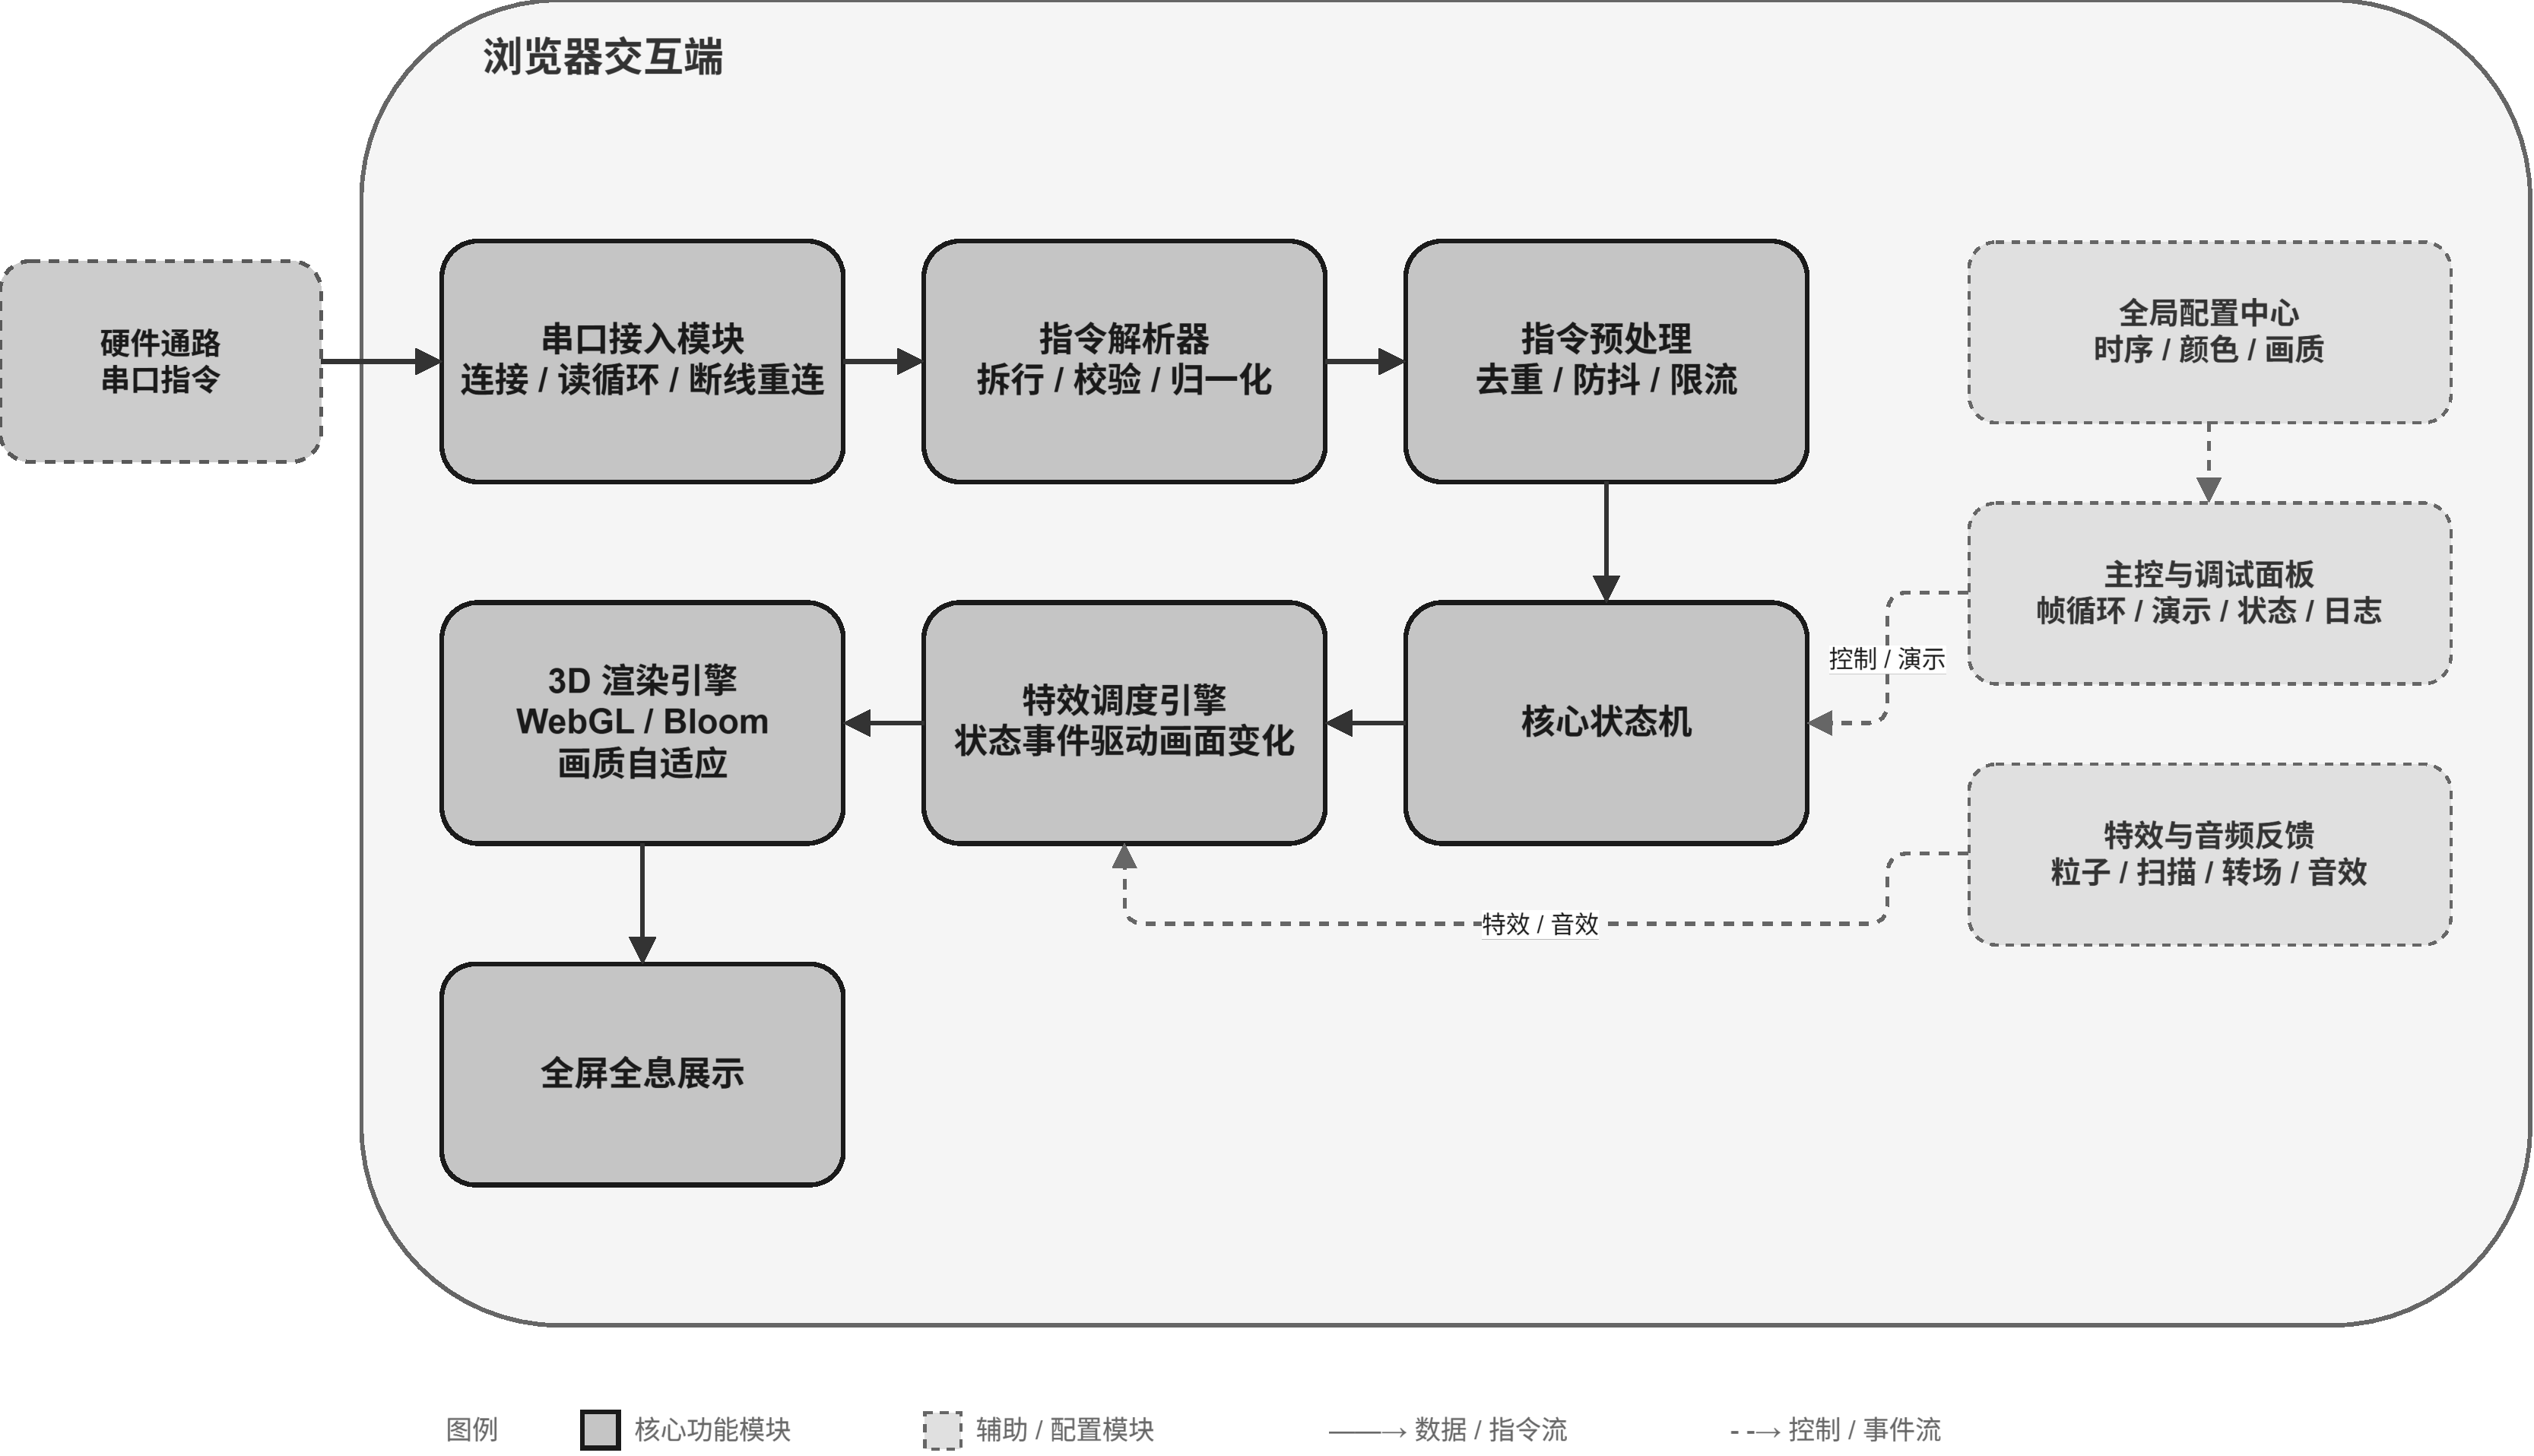
\includegraphics[width=1.10\linewidth,height=0.62\textheight,keepaspectratio]{figures/gesture_web_software_path.pdf}%
  }
  \caption{手势识别与网页控制的软件通路}
  \label{fig:gesture-software-path}
\end{figure}

\section{完成情况及性能参数}
\subsection{整体介绍}
已完成 RV32IM、Zicsr 与基础机器模式指令的数据通路、九级流水线控制、可选 RAS、分级 LSU 和 Store Buffer，并形成仿真及 FPGA 运行记录。
现有板卡运行照片见图~\ref{fig:src0_1_FPGA}、图~\ref{fig:src2_without_FPGA} 和图~\ref{fig:with_FPGA}；整机斜 45 度全局照片尚需补充。
\subsection{工程成果}
\subsubsection{机械成果}
使用现有 FPGA 平台，未独立设计机械部件。
\subsubsection{电路成果}
已形成处理器 RTL、Core\_cpu 封装、存储与外设互连及可加载的 FPGA 工程；当前板级记录覆盖 src0、src1、src2、withMext 与 withoutMext。
RV32F 数据通路和部分运算单元仍在完善，未作为已完成的扩展列入当前测试结论；赛题现场指定的 Z 扩展指令仍待按要求增补。
\subsubsection{软件成果}
已具备镜像转换与加载、Verilator 驱动、IP 模型、IO 显示、指令与程序运行日志、提交统计及 BPU 差分报告。
现有截图同时包含主机测试输出和板卡结果，支持按具体配置核对功能和性能。
\subsection{特性成果}
\paragraph{仿真结果与分析}

\subparagraph{功能验证}

现有报告记录 RV32I 与 RV32M 逐指令测试通过。图~\ref{fig:rv32m-riscv-tests} 展示当前 RV32M 测试输出，8 项均为 PASS；对应版本的 RV32I 逐条测试截图尚需补充。

\begin{figure}[htbp]
  \centering
  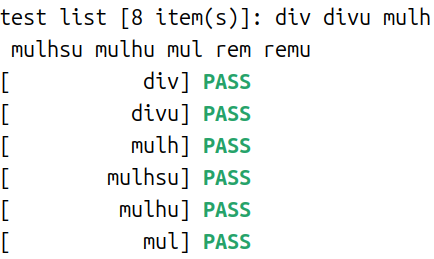
\includegraphics[width=0.90\linewidth,height=0.68\textheight,keepaspectratio]{mext_test_result.png}
  \caption{RV32M riscv-tests 测试结果}
  \label{fig:rv32m-riscv-tests}
\end{figure}

除逐指令测试外，我们还在相同仿真环境中运行了竞业达提供的 src0、src1、src2 和
withMext 程序镜像。四组程序均执行至 \id{HIT GOOD TRAP} 并正常退出，如图
~\ref{fig:jyd-src01-log} 和图~\ref{fig:jyd-src2-mext-log} 所示。日志同时给出了总时钟
周期数、提交指令数和 IPC，说明处理器不仅能够完成基础指令测试，也能够连续运行规模
更大的赛题程序；其中 withMext 的通过还验证了当前数据通路对 RV32M 乘除法指令的支持。

\begin{figure}[htbp]
  \centering
  \begin{minipage}{0.48\linewidth}
    \centering
    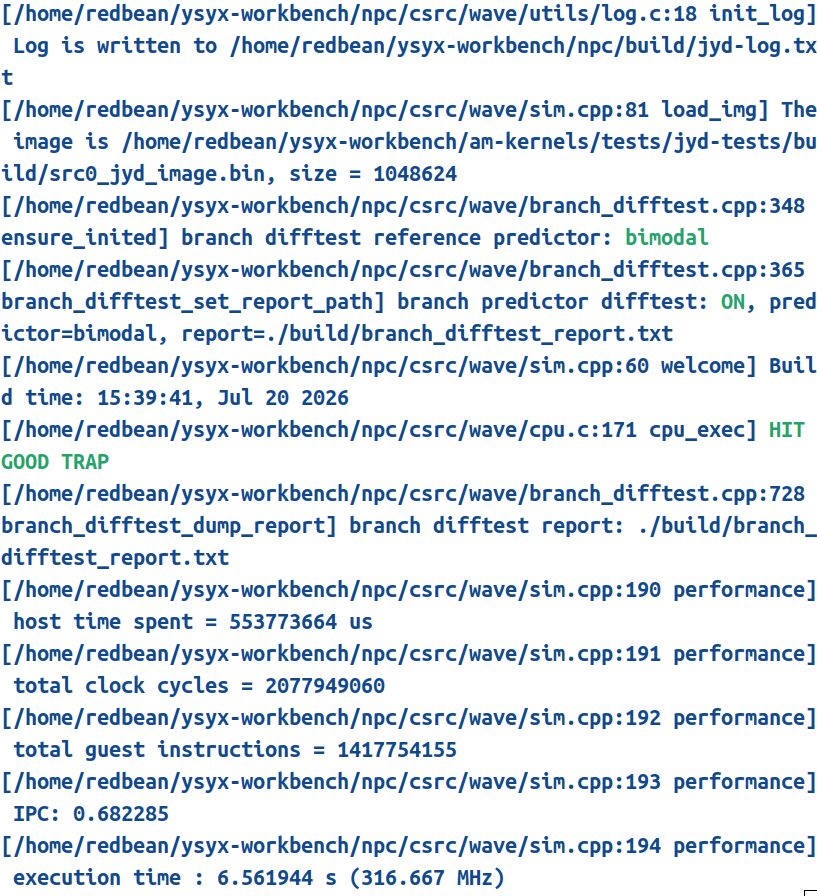
\includegraphics[width=\linewidth,height=0.68\textheight,keepaspectratio]{src0_jyd_log.png}
    \caption*{(a) src0}
  \end{minipage}
  \hfill
  \begin{minipage}{0.48\linewidth}
    \centering
    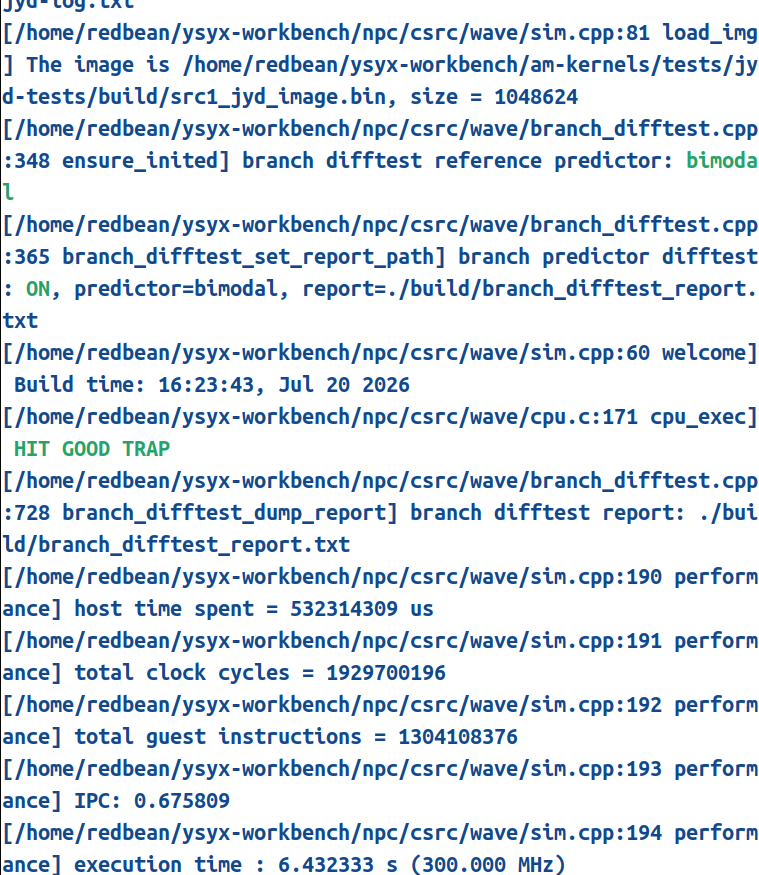
\includegraphics[width=\linewidth,height=0.68\textheight,keepaspectratio]{src1_jyd_log.png}
    \caption*{(b) src1}
  \end{minipage}
  \par\medskip
  \caption{竞业达 src0 与 src1 程序仿真结果}
  \label{fig:jyd-src01-log}
\end{figure}

\begin{figure}[htbp]
  \centering
  \begin{minipage}{0.48\linewidth}
    \centering
    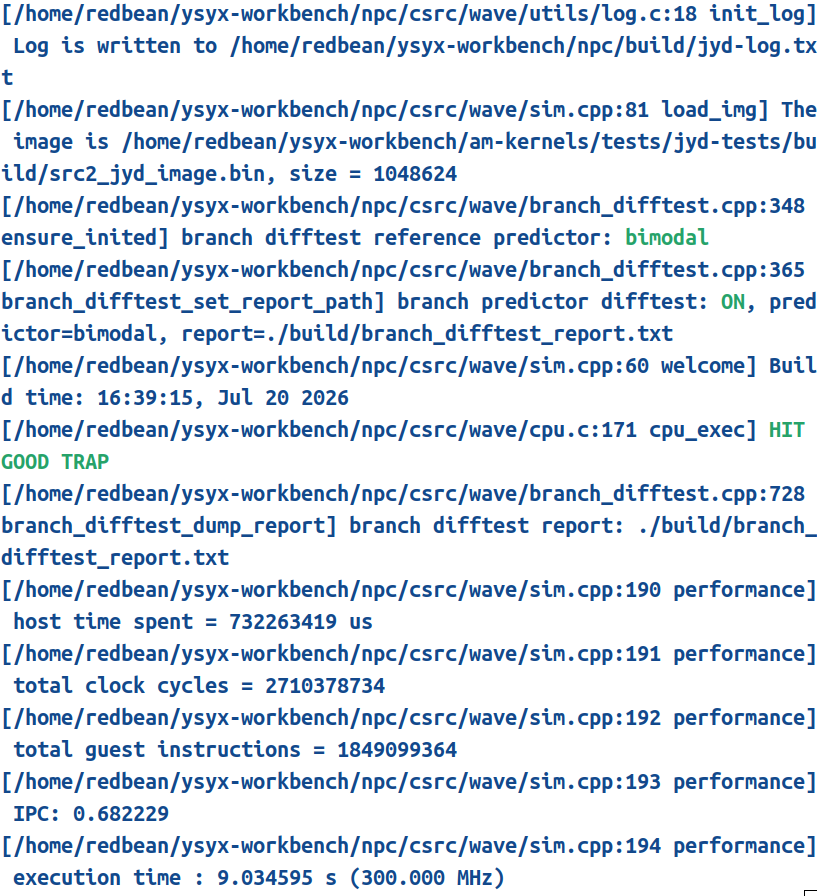
\includegraphics[width=\linewidth,height=0.68\textheight,keepaspectratio]{src2_jyd_log.png}
    \caption*{(a) src2}
  \end{minipage}
  \hfill
  \begin{minipage}{0.48\linewidth}
    \centering
    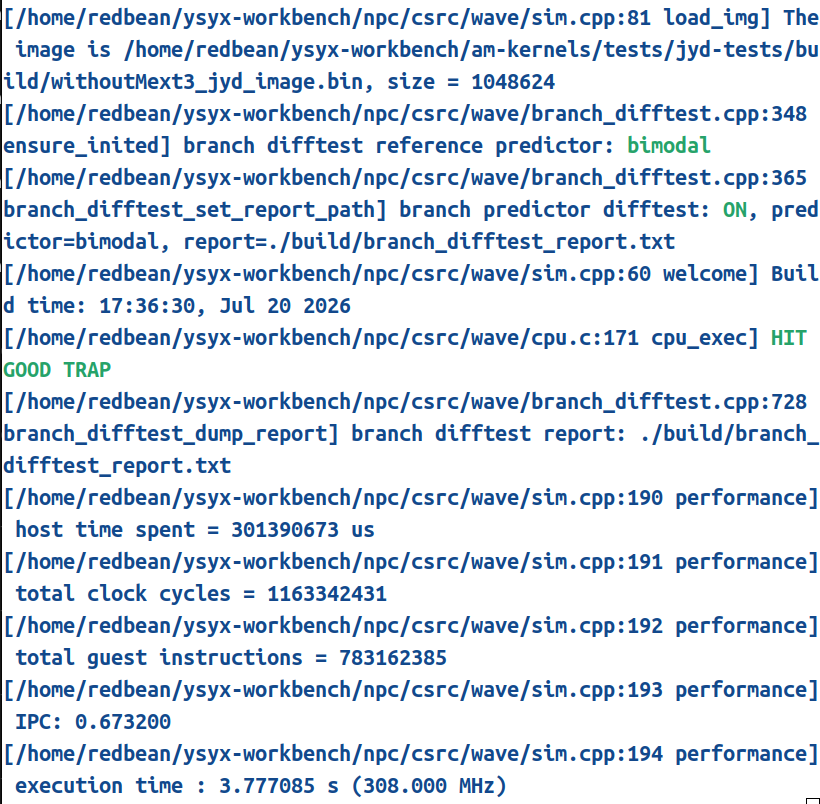
\includegraphics[width=\linewidth,height=0.68\textheight,keepaspectratio]{without_jyd_log.png}
    \caption*{(b) withoutMext}
  \end{minipage}
  \par\medskip
  \caption{竞业达 src2 与 withoutMext 程序仿真结果}
  \label{fig:jyd-src2-mext-log}
\end{figure}

\begin{figure}[htbp]
  \centering
  \hfill
  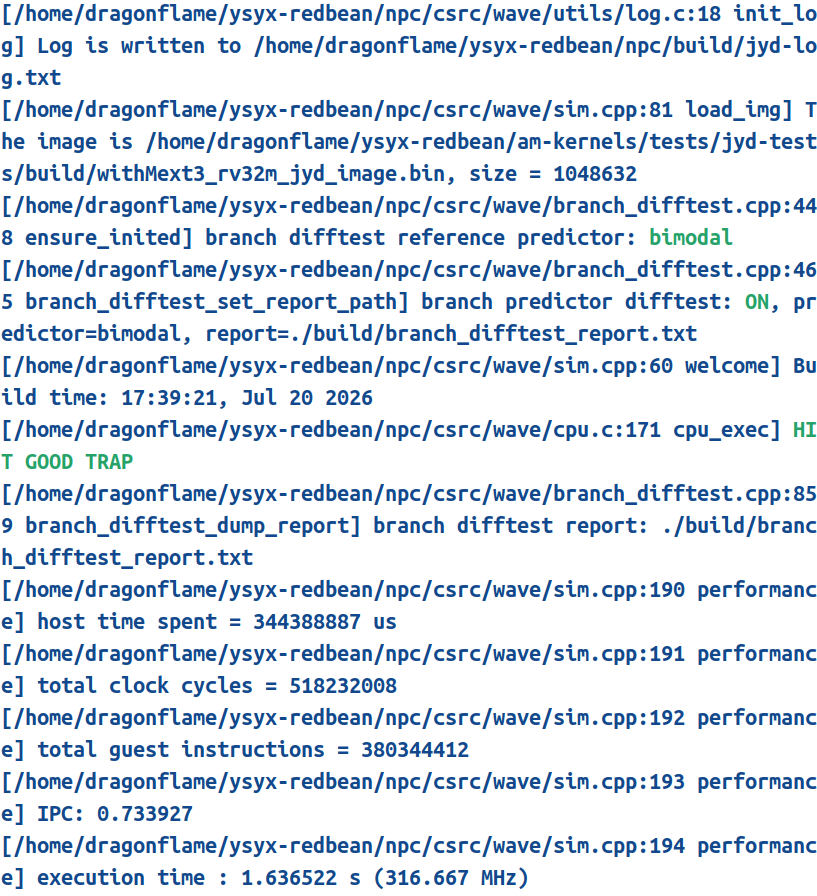
\includegraphics[width=\linewidth,height=0.68\textheight,keepaspectratio]{withMext3_jyd_log.png}
  \caption{竞业达 withMext 程序仿真结果}
  \label{fig:jyd-mext-log}
\end{figure}

\subparagraph{分支预测器验证与预测收益分析}

分支预测差分框架分别以纯 Bimodal/BTB 和 Bimodal/BTB+RAS 两种配置运行同一测试
镜像，并逐事件比较 RTL 与 C++ 参考模型给出的方向和目标。在现有各组报告中，两种配置
的模型匹配率均为 100\%，说明新增的返回指令标记、RAS 更新以及目标覆盖逻辑与参考
模型一致。

当 CoreMark 在未使用原生 RV32M 乘除法指令的代码流上测试时，乘除运算需要
通过软件例程完成，由于数据的随机性，位移乘法会导致分支预测难以进行。在没有乘除指令的情况下，
CoreMark 使用 Bimodal 预测条件分支、跳转和总体准确率分别为 70.26\%、74.72\% 和 70.75\%。当前测试镜像直接
使用硬件 \code{mul}/\code{div} 等 RV32M 指令，不再通过软乘除例程模拟同类运算；
在关闭 RAS、仍采用 256 项 Bimodal/BTB 的情况下，三项准确率分别达到 92.48\%、
94.65\% 和 92.75\%，对比如表~\ref{tab:bpu-old-current} 所示。

\begin{table}[H]
  \centering
  \caption{ CoreMark 的 Bimodal 预测结果对比}
  \label{tab:bpu-old-current}
  \begin{adjustbox}{max width=\linewidth}
\begin{tabular}{lrrr}
    \toprule
    CoreMark 代码流 & 条件分支准确率 & 跳转准确率 & 总体准确率 \\
    \midrule
    软件乘除例程 & 70.26\% & 74.72\% & 70.75\% \\
    原生 RV32M & 92.48\% & 94.65\% & 92.75\% \\
    \bottomrule
  \end{tabular}
\end{adjustbox}
\end{table}

原生乘除法指令缩短了动态指令序列，并减少软乘除函数调用、返回以及循环分支对 BTB
表项的占用和冲突，使剩余控制流更集中、更容易被 Bimodal/BTB 学习。因此，当前代码流
的总体准确率较之前提高 22.00 个百分点。

在此基础上，表~\ref{tab:bpu-ras-comparison} 使用相同 RV32M 镜像(即含有乘除法指令)进一步比较 RAS
开关造成的变化，从而单独评价 RAS 的收益。

\begin{table}[H]
  \centering
  \caption{Bimodal/BTB 与 Bimodal/BTB+RAS 预测结果对比}
  \label{tab:bpu-ras-comparison}
  \begin{adjustbox}{max width=\linewidth}
\begin{tabular}{llrrr}
    \toprule
    测试程序 & RAS & 条件分支准确率 & 跳转准确率 & 总体准确率 \\
    \midrule
    CoreMark & 关闭 & 92.48\% & 94.65\% & 92.75\% \\
    CoreMark & 开启 & 92.48\% & 98.98\% & 93.30\% \\
    \midrule
    src0 RV32M & 关闭 & 99.39\% & 99.93\% & 99.39\% \\
    src0 RV32M & 开启 & 99.39\% & 99.94\% & 99.39\% \\
    src1 RV32M & 关闭 & 97.11\% & 100.00\% & 97.31\% \\
    src1 RV32M & 开启 & 97.11\% & 100.00\% & 97.31\% \\
    \midrule
    src2 RV32M & 关闭 & 79.35\% & 99.96\% & 82.88\% \\
    src2 RV32M & 开启 & 79.35\% & 100.00\% & 82.89\% \\
    withMext RV32M & 关闭 & 98.77\% & 99.84\% & 98.79\% \\
    withMext RV32M & 开启 & 98.77\% & 99.86\% & 98.79\% \\
    \bottomrule
  \end{tabular}
\end{adjustbox}
\end{table}

CoreMark 中函数调用与返回较为频繁，因此最能体现 RAS 的收益。关闭 RAS 时，
7,704,471 次跳转更新中有 412,430 次预测错误；启用 8 项 RAS 后，正确预测数由
7,292,041 增加到 7,626,169，跳转错误数降至 78,302。对应的跳转
准确率提高 4.33 个百分点，并使总体准确率从 92.75\% 提高到 93.30\%。图
~\ref{fig:coremark-ras-comparison} 给出了两种配置下的完整报告。

\begin{figure}[htbp]
  \centering
  \begin{minipage}{0.48\linewidth}
    \centering
    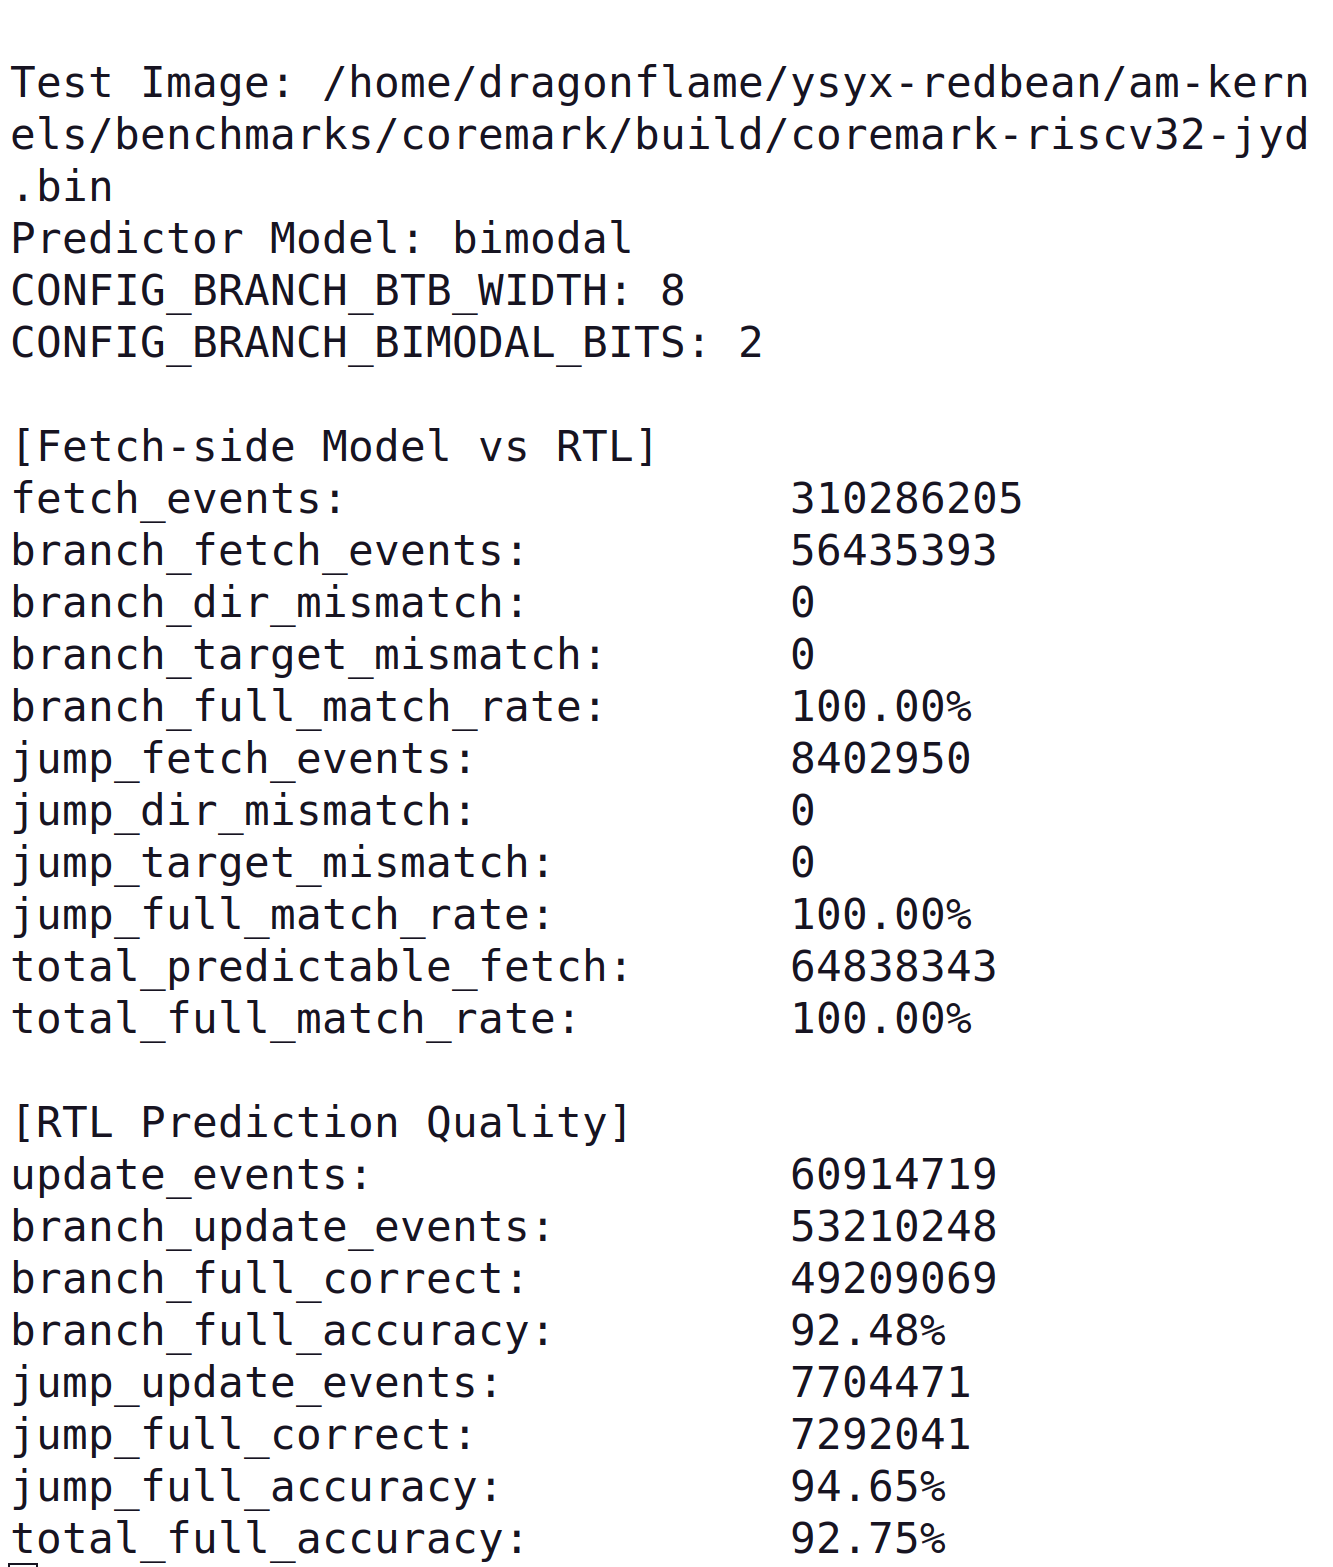
\includegraphics[width=\linewidth,height=0.68\textheight,keepaspectratio]{core_branch.png}
    \caption*{(a) 关闭 RAS}
  \end{minipage}
  \hfill
  \begin{minipage}{0.48\linewidth}
    \centering
    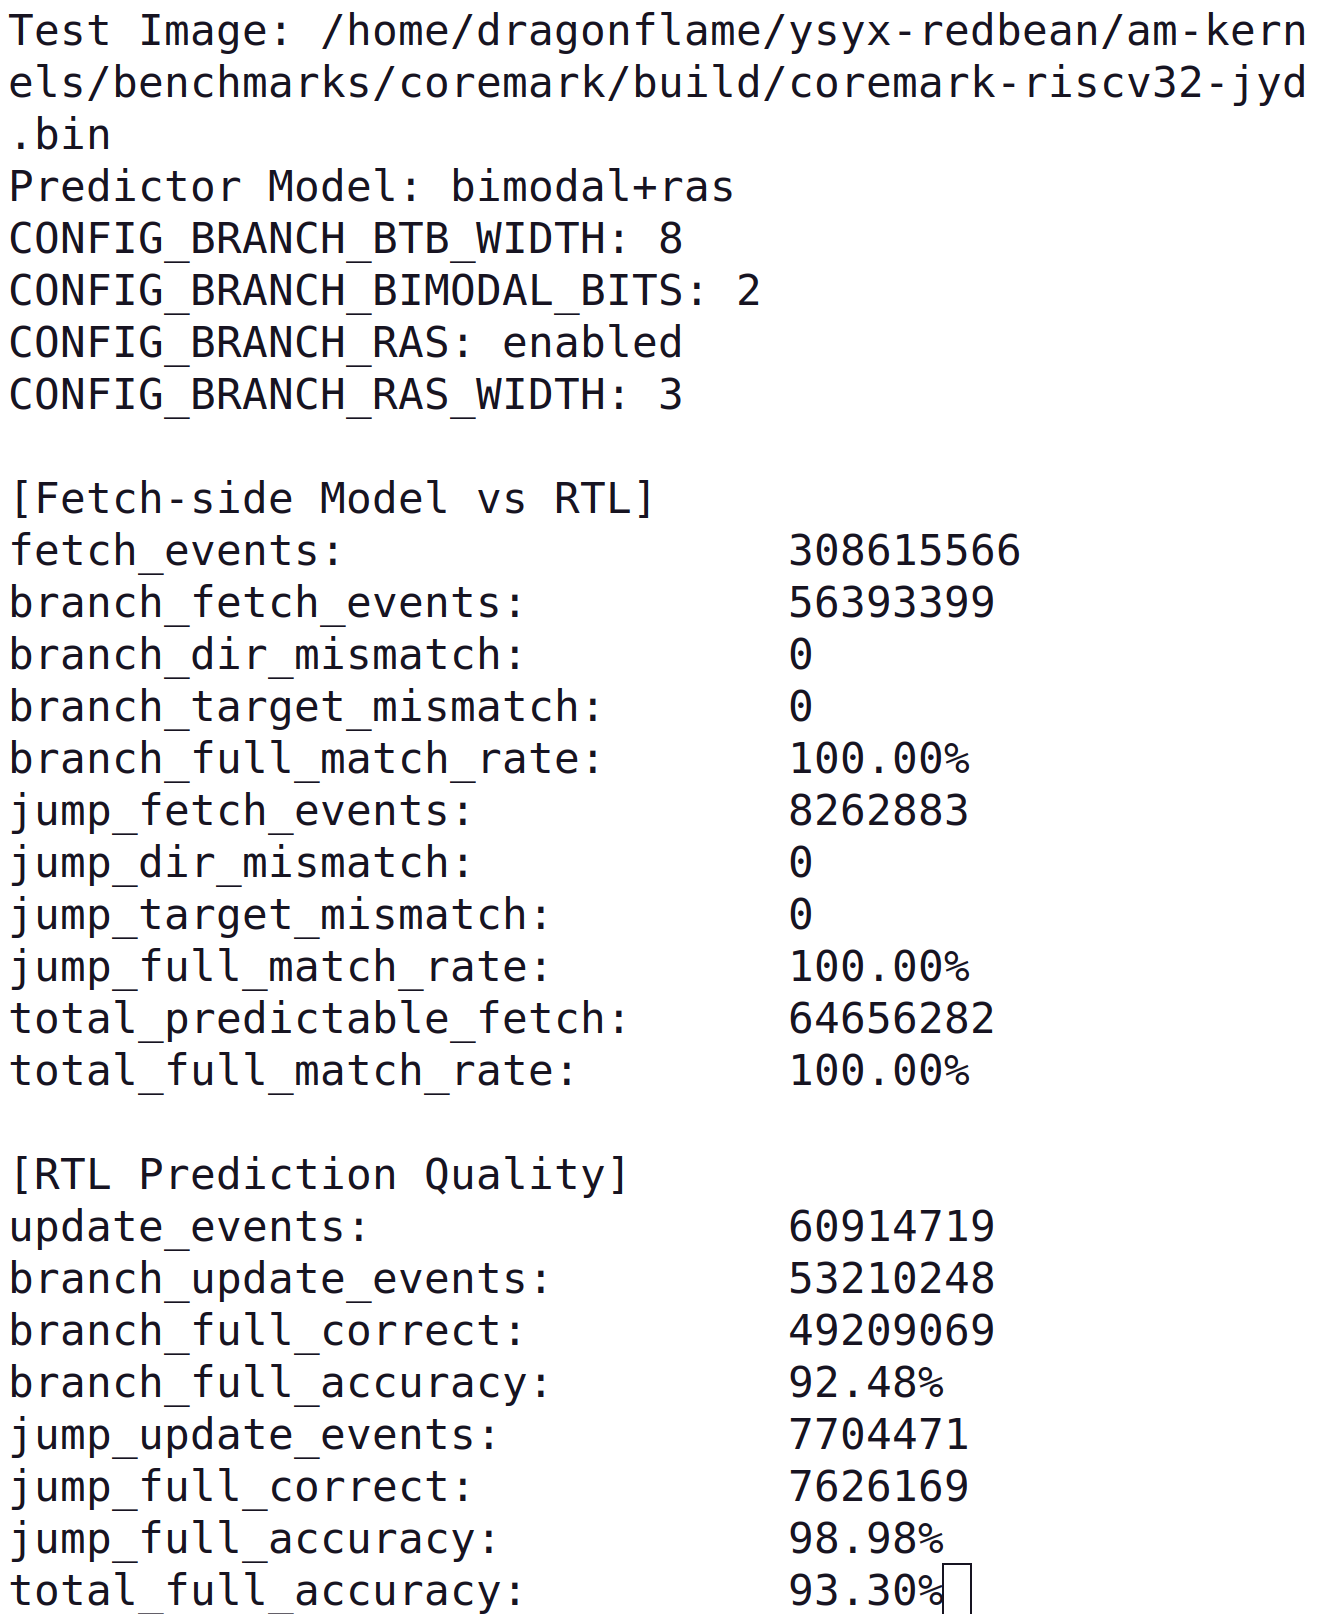
\includegraphics[width=\linewidth,height=0.68\textheight,keepaspectratio]{core_ras_branch.png}
    \caption*{(b) 开启 RAS}
  \end{minipage}
  \caption{CoreMark 中 RAS 对分支预测结果的影响}
  \label{fig:coremark-ras-comparison}
\end{figure}

src2 中条件分支事件占比较高，且其 79.35\% 的方向/目标预测结果不受 RAS 影响，
因此 RAS 对总体准确率的提升仅在四舍五入后表现为 0.01 个百分点。不过，跳转错误仍由
4,756 次减少到 158 次，减少约 96.7\%，说明 RAS 对返回地址的预测本身有效，只是其
收益被数量更多的条件分支事件稀释。对应结果见图~\ref{fig:src2-ras-comparison}。

\begin{figure}[htbp]
  \centering
  \begin{minipage}{0.48\linewidth}
    \centering
    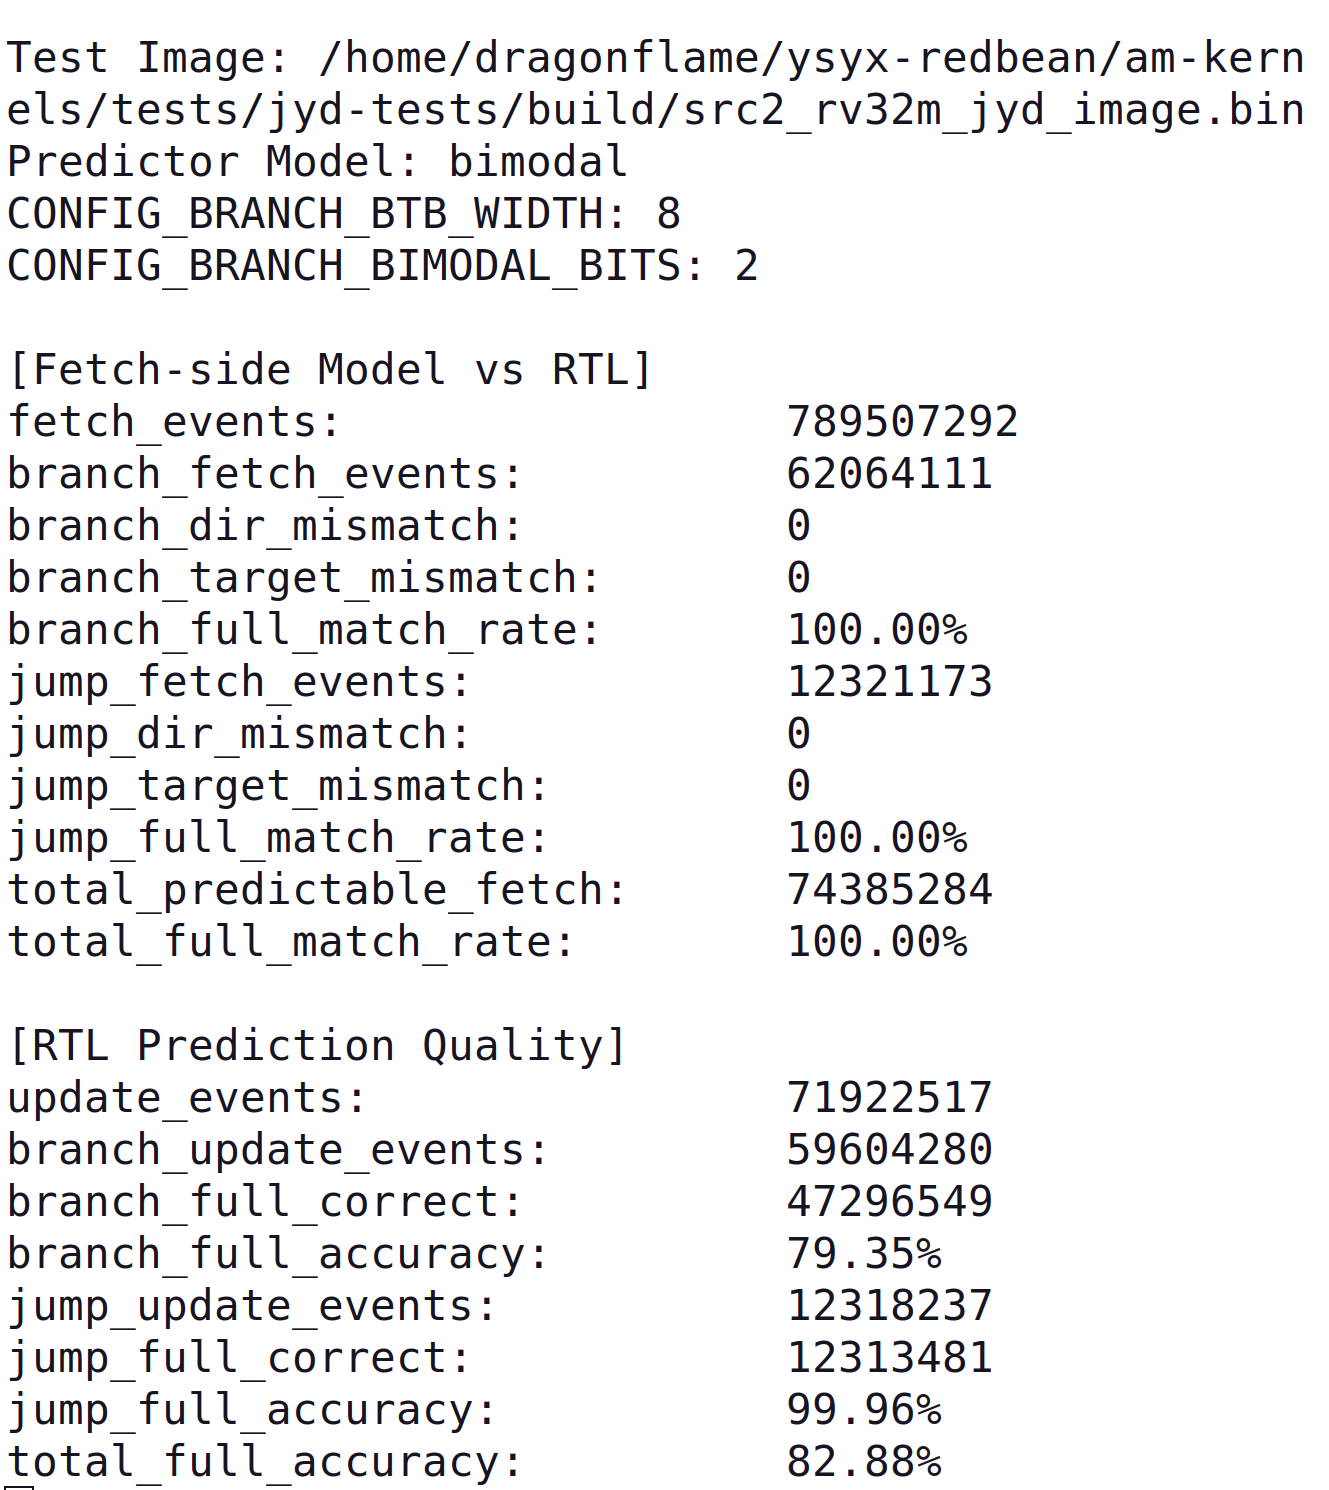
\includegraphics[width=\linewidth,height=0.68\textheight,keepaspectratio]{src2_branch.png}
    \caption*{(a) 关闭 RAS}
  \end{minipage}
  \hfill
  \begin{minipage}{0.48\linewidth}
    \centering
    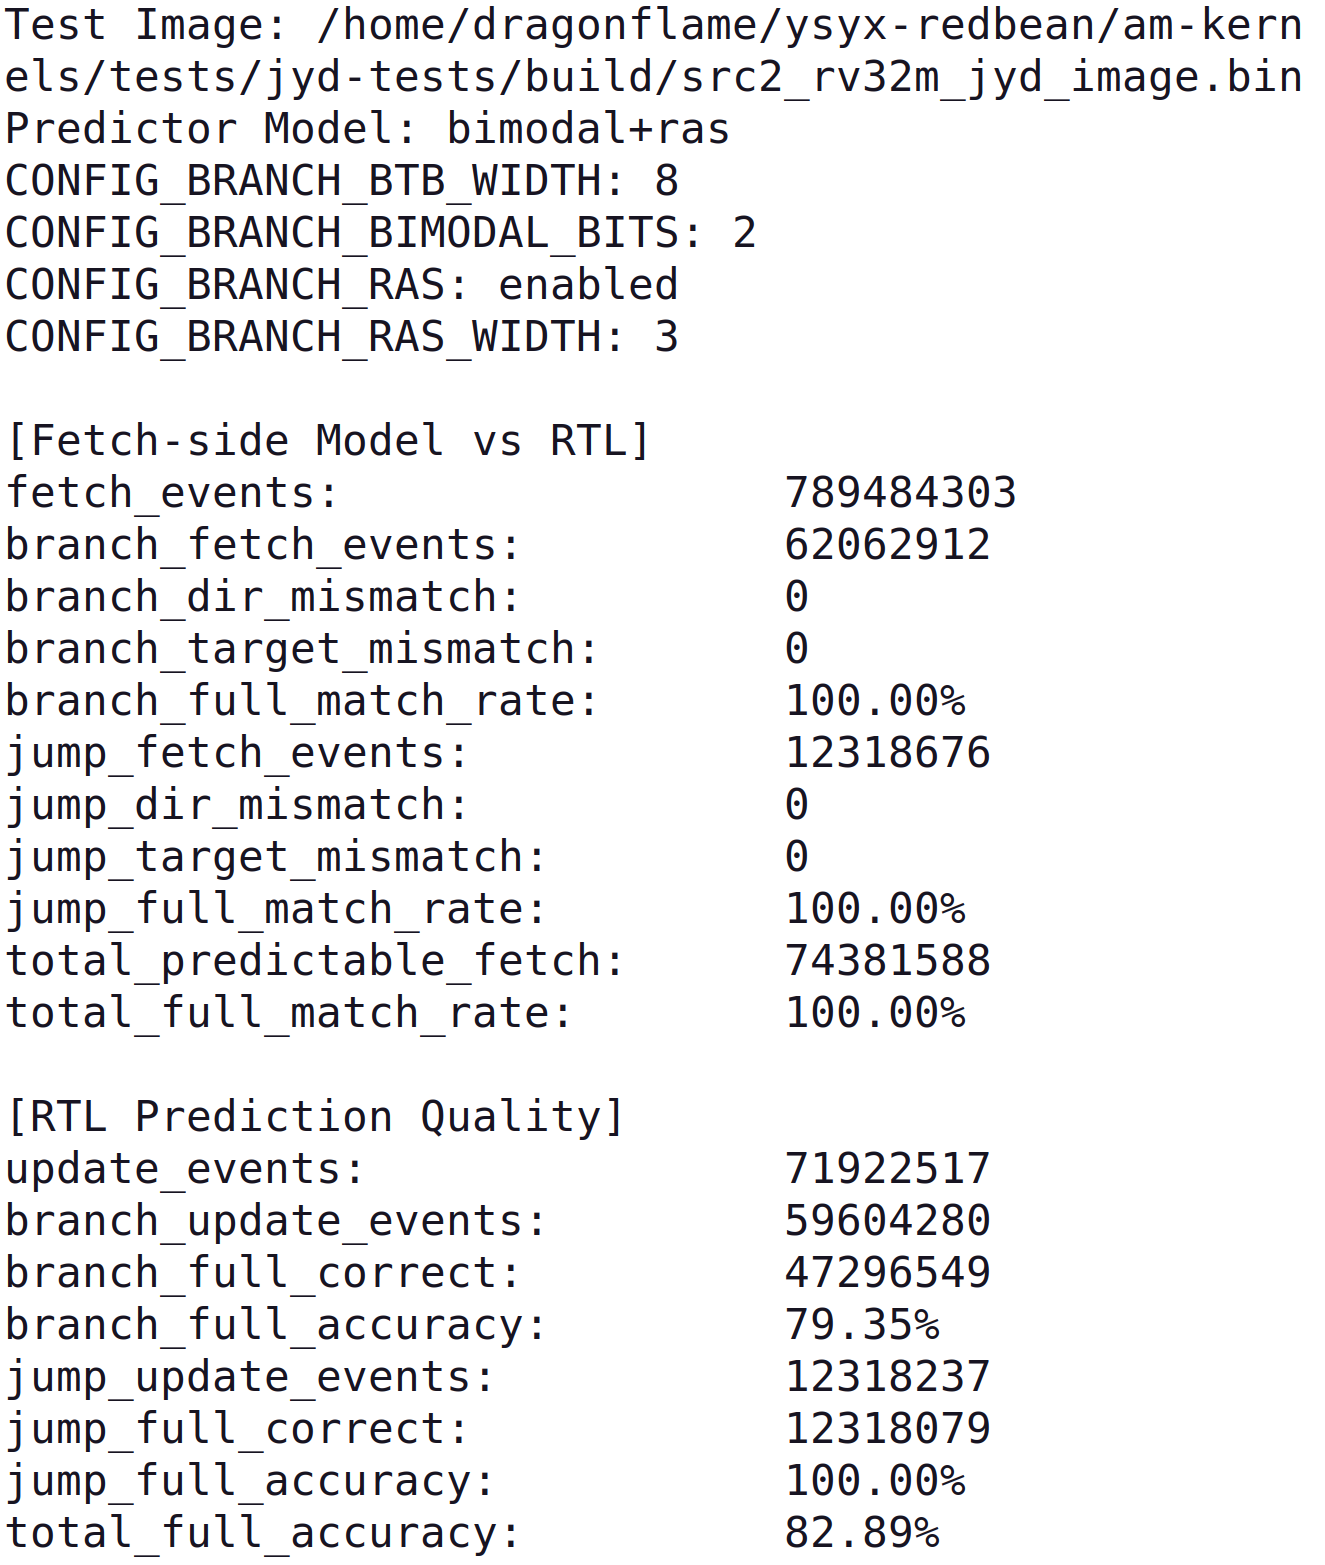
\includegraphics[width=\linewidth,height=0.68\textheight,keepaspectratio]{src2_ras_branch.png}
    \caption*{(b) 开启 RAS}
  \end{minipage}
  \caption{src2 RV32M 中 RAS 对分支预测结果的影响}
  \label{fig:src2-ras-comparison}
\end{figure}

src0、src1 和 withMext 在关闭 RAS 时的跳转准确率已经分别达到 99.93\%、100.00\%
和 99.84\%，说明采用原生 RV32M 指令后，这些程序中的跳转目标已经较容易由 BTB 预测。
RAS 使 src0 的跳转错误由 183 次减少到 163 次，使 src1 的跳转错误由 158 次减少到
154 次；withMext 的跳转准确率则进一步提高至 99.86\%。由于三者的基础准确率已经
很高，改进反映到总体准确率上均不足以在保留两位小数时体现。

\begin{figure}[htbp]
  \centering
  \begin{minipage}{0.48\linewidth}
    \centering
    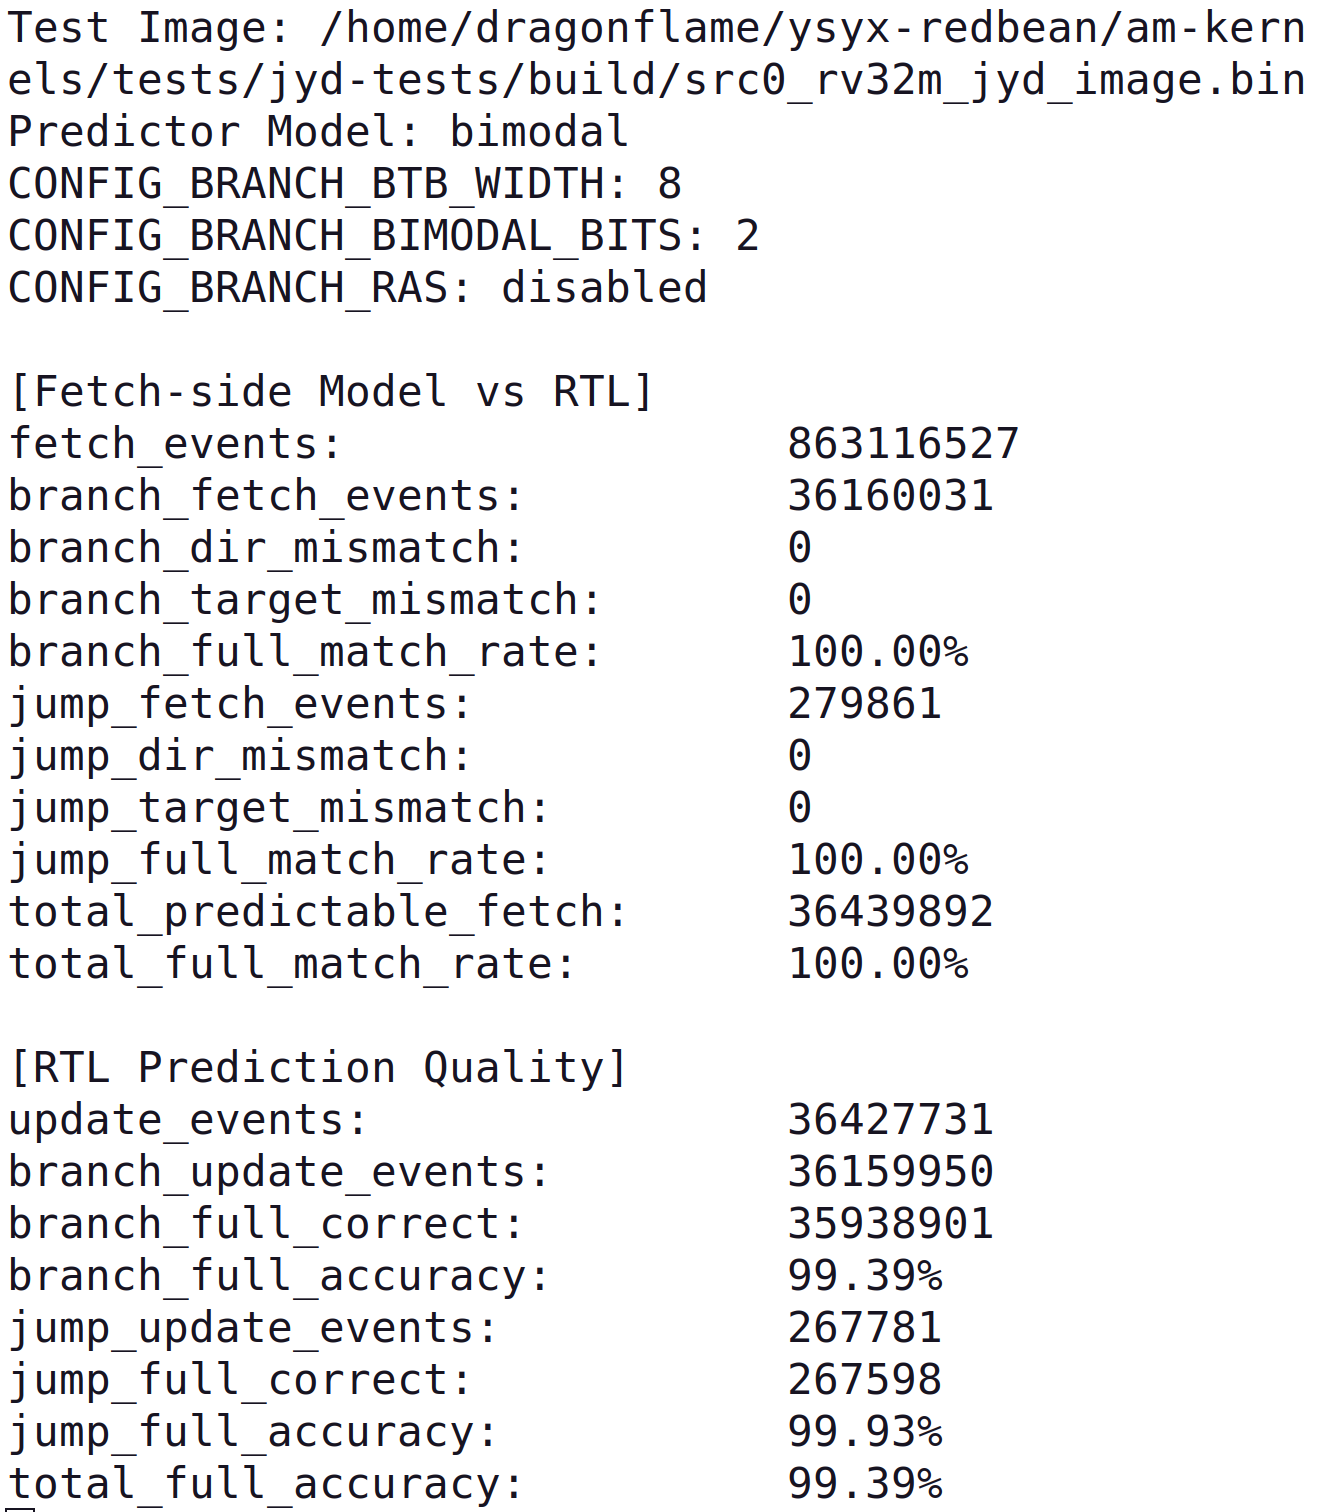
\includegraphics[width=\linewidth,height=0.68\textheight,keepaspectratio]{src0_branch.png}
    \caption*{(a) src0，关闭 RAS}
  \end{minipage}
  \hfill
  \begin{minipage}{0.48\linewidth}
    \centering
    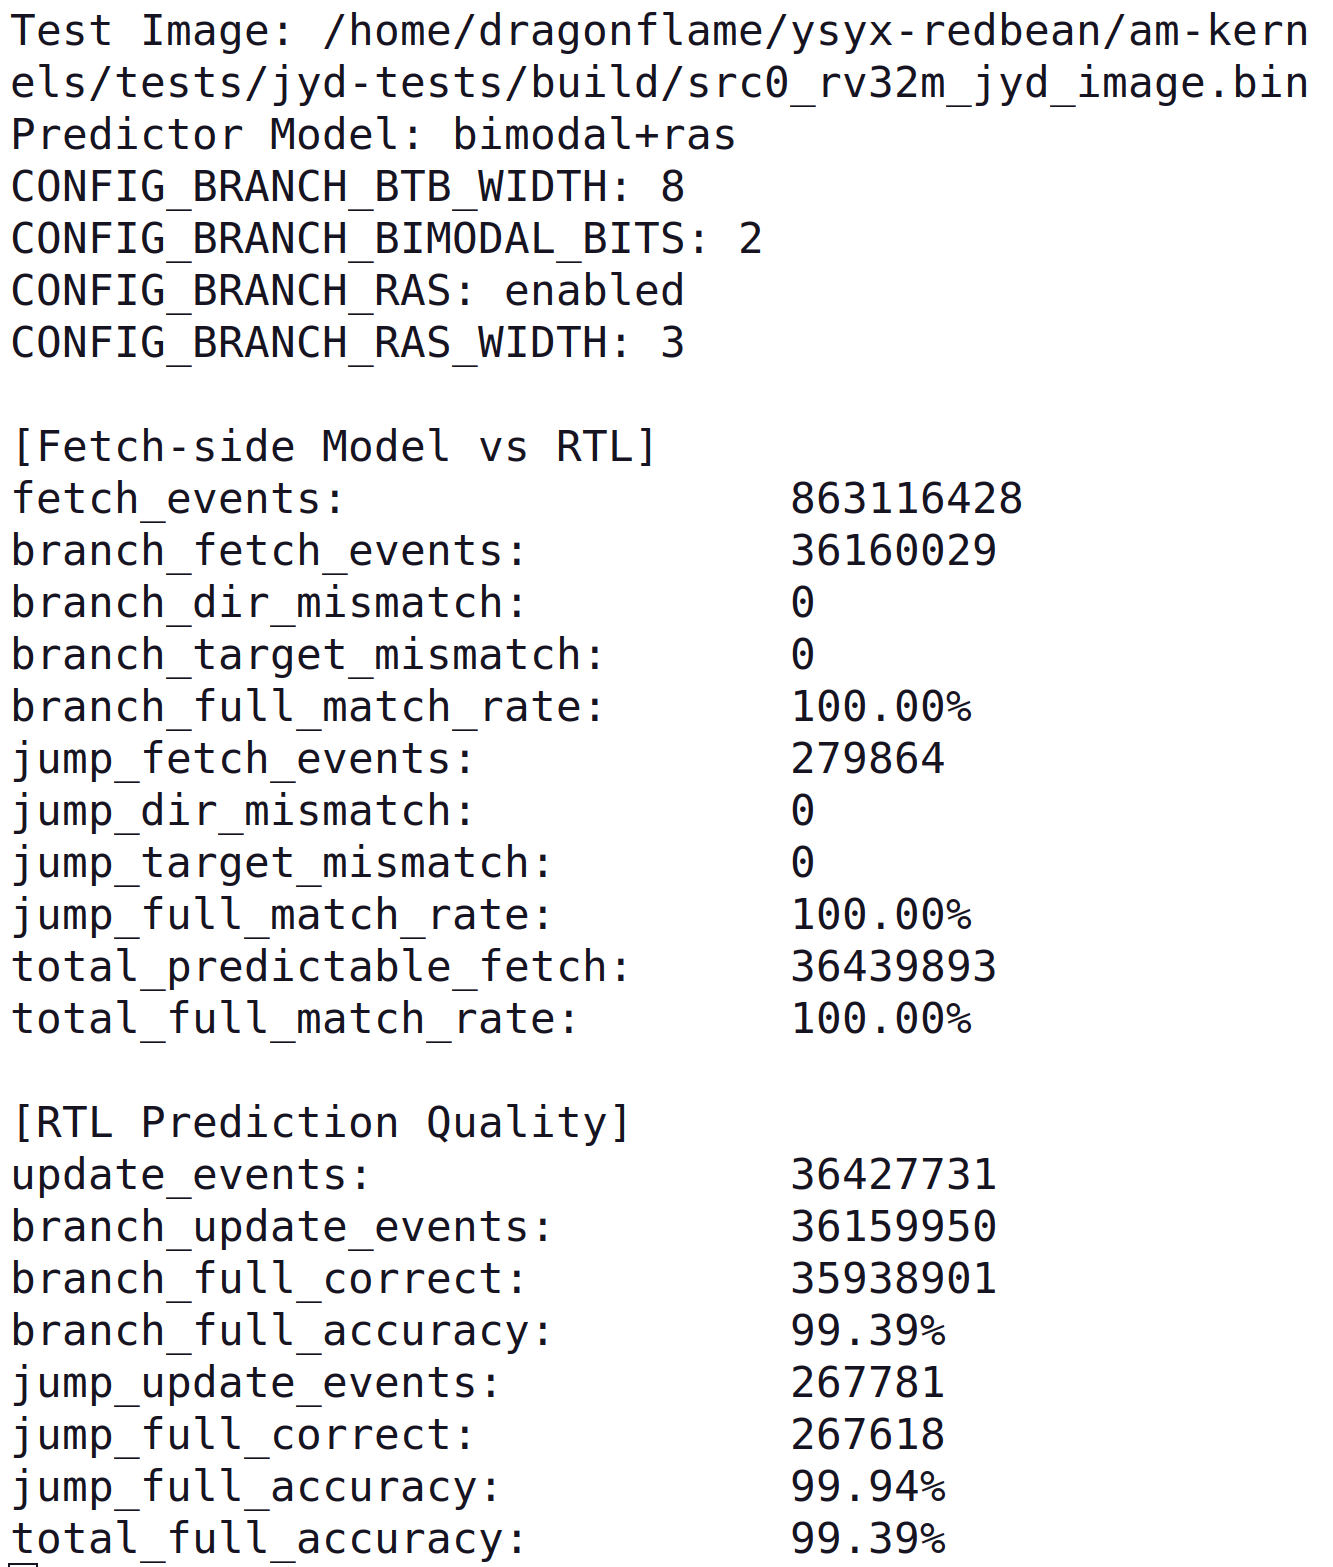
\includegraphics[width=\linewidth,height=0.68\textheight,keepaspectratio]{src0_ras_branch.png}
    \caption*{(b) src0，开启 RAS}
  \end{minipage}
  \caption{src0 RV32M 中 RAS 对分支预测结果的影响}
  \label{fig:src0-ras-comparison}
\end{figure}

\begin{figure}[htbp]
  \centering
  \begin{minipage}{0.48\linewidth}
    \centering
    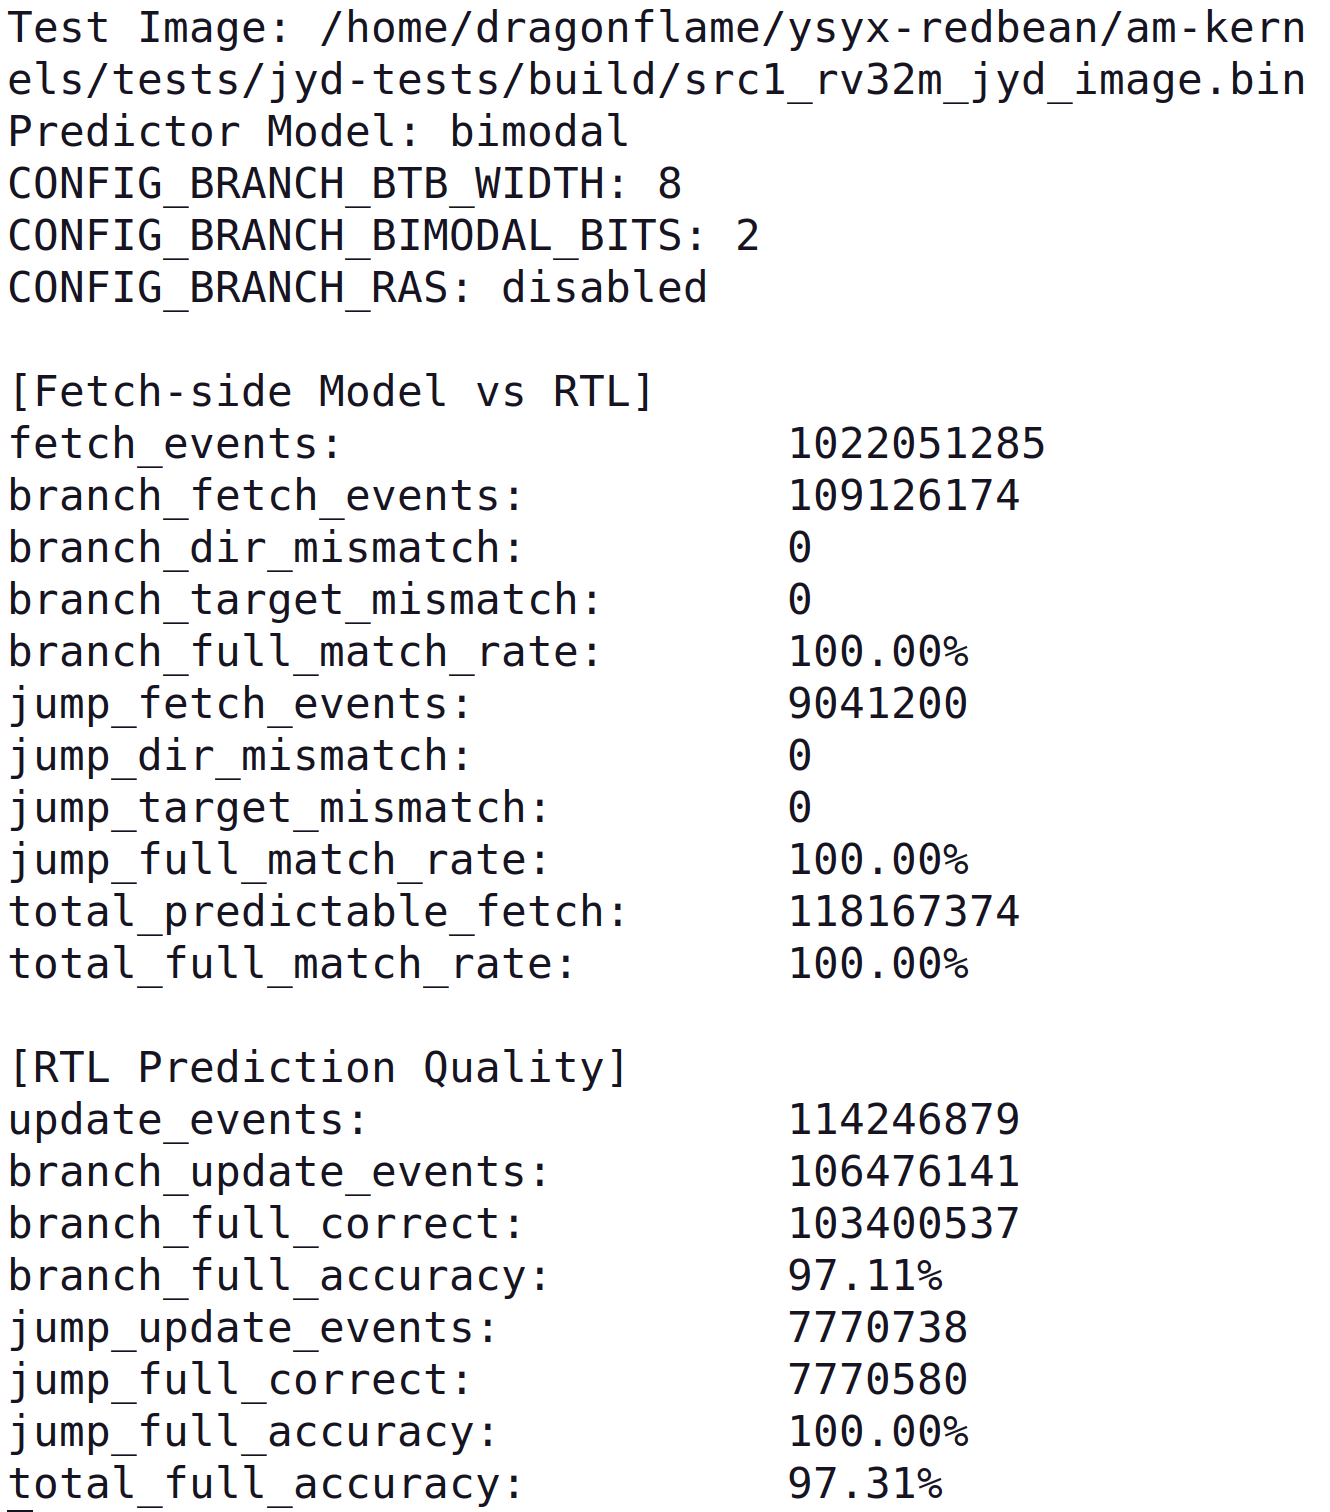
\includegraphics[width=\linewidth,height=0.68\textheight,keepaspectratio]{src1_branch.png}
    \caption*{(a) src1，关闭 RAS}
  \end{minipage}
  \hfill
  \begin{minipage}{0.48\linewidth}
    \centering
    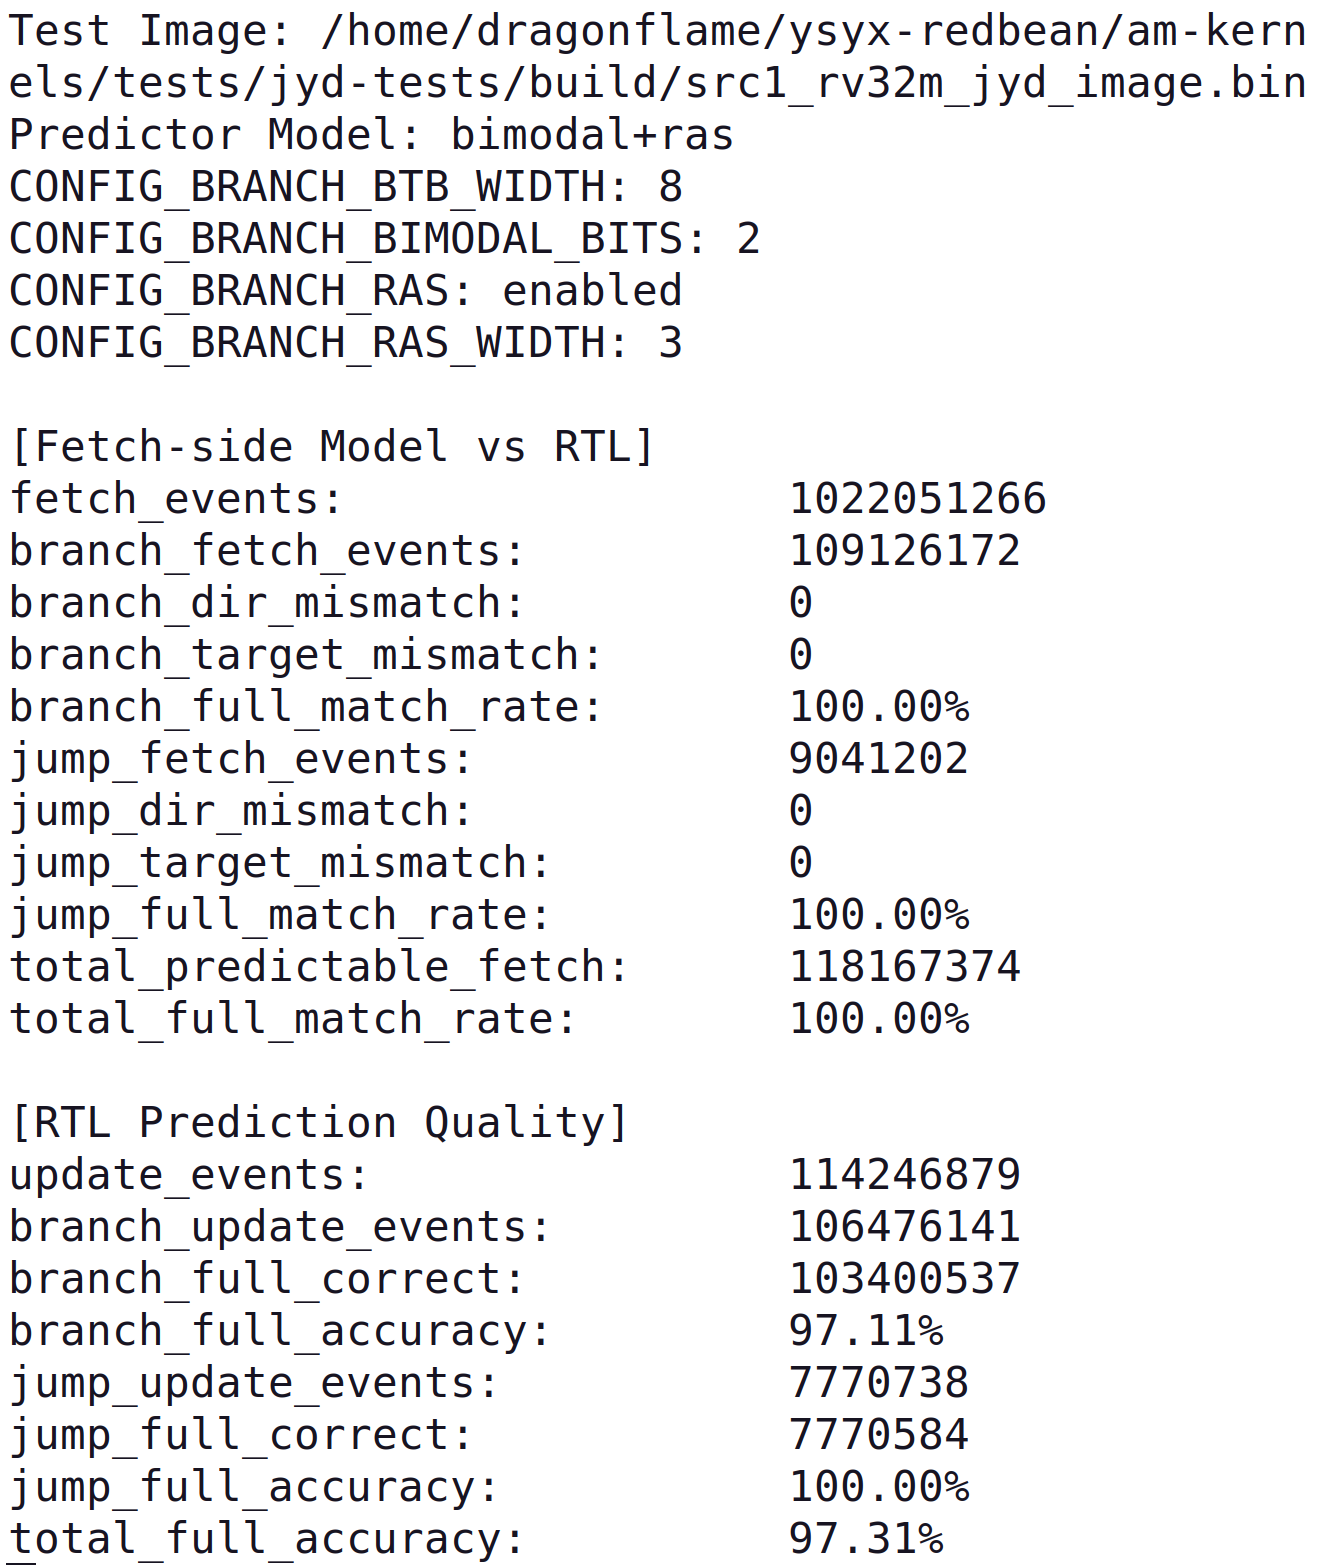
\includegraphics[width=\linewidth,height=0.68\textheight,keepaspectratio]{src1_ras_branch.png}
    \caption*{(b) src1，开启 RAS}
  \end{minipage}
  \caption{src1 RV32M 中 RAS 对分支预测结果的影响}
  \label{fig:src1-ras-comparison}
\end{figure}

\begin{figure}[htbp]
  \centering
  \begin{minipage}{0.48\linewidth}
    \centering
    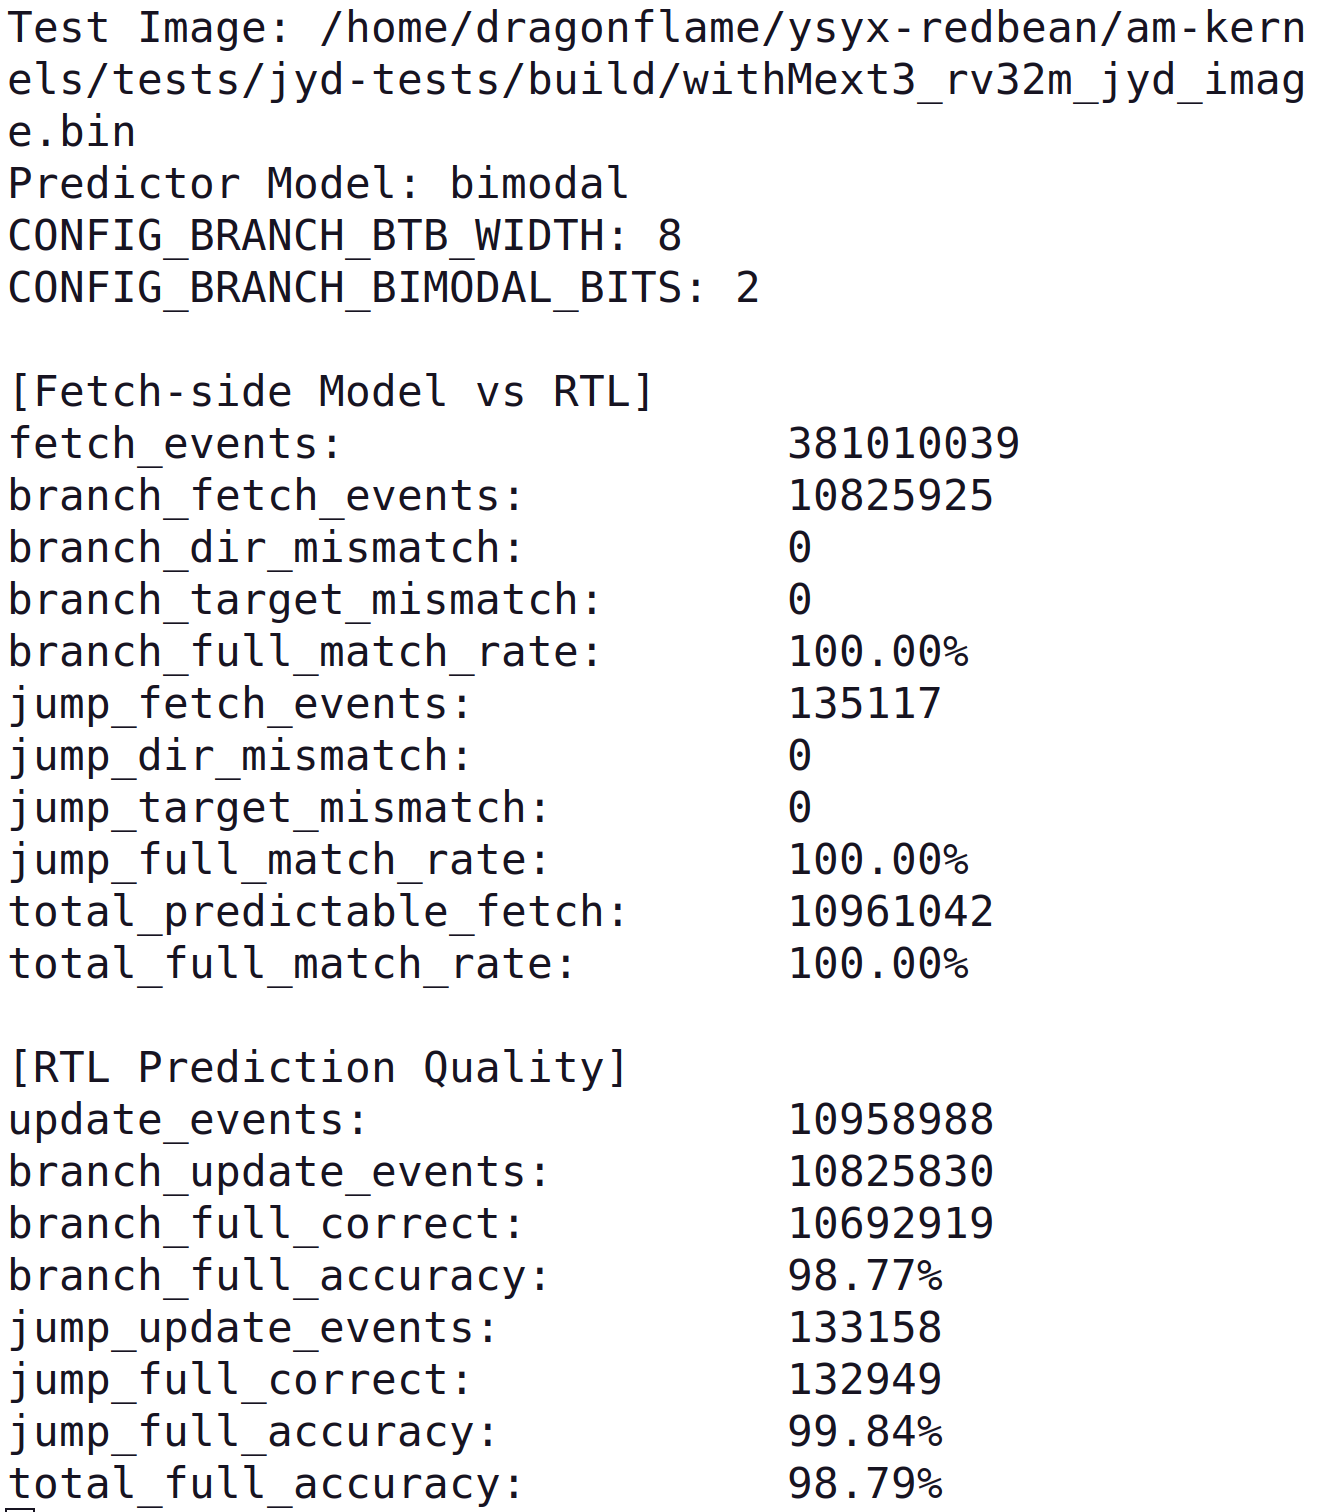
\includegraphics[width=\linewidth,height=0.68\textheight,keepaspectratio]{withMext3_branch.png}
    \caption*{(a) withMext，关闭 RAS}
  \end{minipage}
  \hfill
  \begin{minipage}{0.48\linewidth}
    \centering
    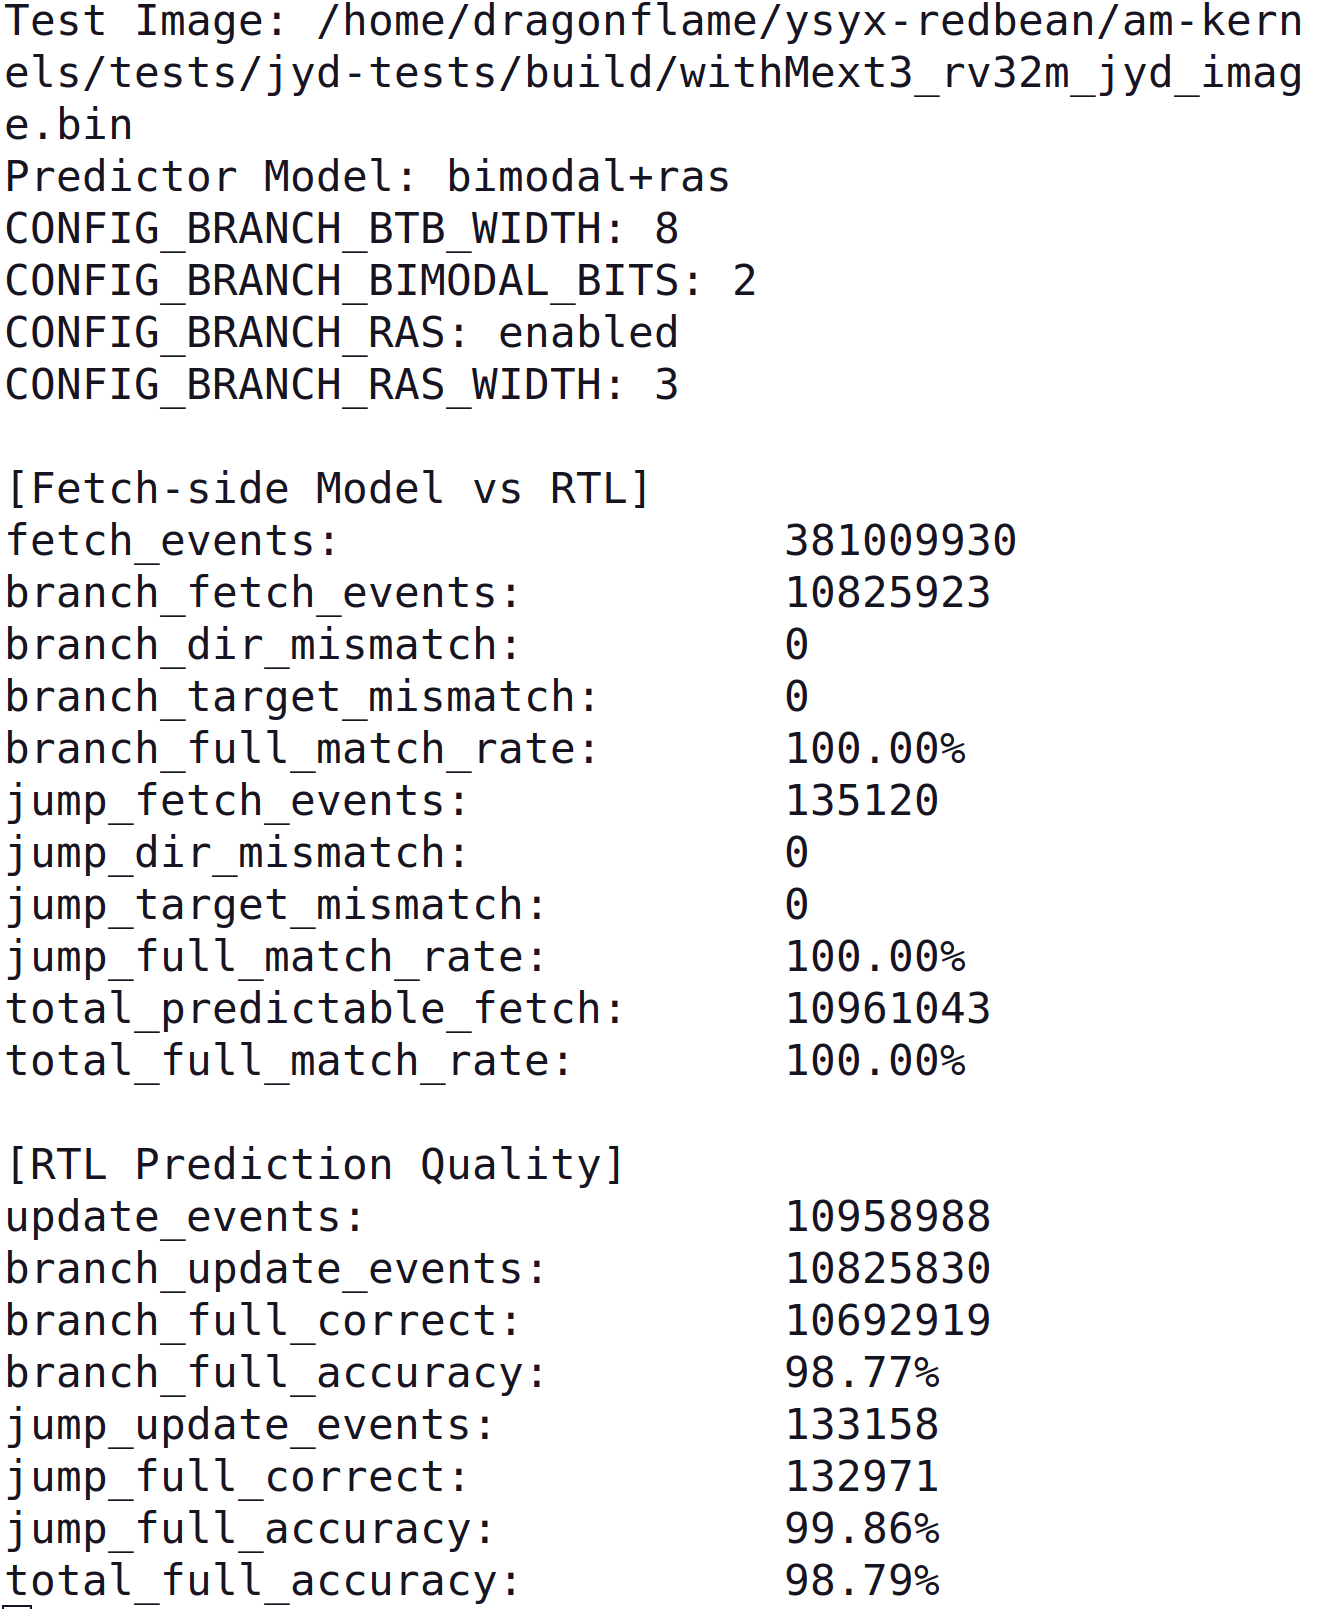
\includegraphics[width=\linewidth,height=0.68\textheight,keepaspectratio]{withMext3_ras_branch.png}
    \caption*{(b) withMext，开启 RAS}
  \end{minipage}
  \caption{withMext RV32M 中 RAS 对分支预测结果的影响}
  \label{fig:withmext3-ras-comparison}
\end{figure}

综合来看，原生 RV32M 指令通过消除软乘除例程，简化了程序的动态控制流，使当前
Bimodal/BTB 相比旧文档中的测试更容易获得较高准确率；RAS 则是在相同代码流上进一步
针对函数返回目标进行优化，不改变条件分支的 Bimodal 方向预测。其收益取决于返回指令
的频率及原 BTB 对返回目标的预测质量：CoreMark 的跳转准确率提高 4.33 个百分点，收益
最明显；src0、src1、src2 和 withMext 的基础跳转准确率已经接近 100\%，因此总体收益
较小。这一结果说明，RAS 对调用返回密集型负载具有明确价值，而将其设计为可选配置，
可以让资源或时序更敏感的场景继续使用结构更简单的 Bimodal/BTB。

\paragraph{FPGA 验证}

\subparagraph{硬件平台说明}

验证平台为竞业达 FPGA 试验箱的数字孪生平台，目标器件为 Xilinx Kintex-7，
工程使用 Vivado 2023.2 完成综合、实现和 bitstream 生成。

\subparagraph{运行流程说明}

FPGA 验证流程包括：生成当前 SystemVerilog；将处理器和 SoC 文件加入 Vivado 工程；
更新 IROM/DRAM 初始化文件；生成或更新 IP 输出产物；执行综合、实现和时序检查；生成
bitstream；在数字孪生平台加载工程；最后观察 LED、数码管和计数结果。

\subparagraph{测试用例说明}

赛方以 \id{irom.coe} 和 \id{dram.coe} 提供测试镜像。IROM 镜像包含启动代码、
指令测试和控制流程，DRAM 镜像提供初始数据。区域赛测试依次覆盖 RV32I/RV32IM、
CSR/trap 和性能程序，LED 用于显示各测试项状态，数码管显示通过条数和运行时间。

\begin{figure}[htbp]
  \centering
  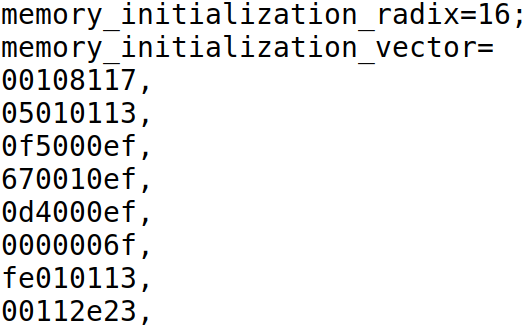
\includegraphics[width=0.72\linewidth,height=0.68\textheight,keepaspectratio]{withMext}
  \caption{withMext IROM 初始化文件的部分内容}
  \label{fig:irom-coe-example}
\end{figure}

\paragraph{FPGA 验证结果及分析}

\subparagraph{FPGA 上板验证结果}

集成于官方 SoC 上的九级流水处理器在上板测试中正常运行。多次验证结果表明
RV32I 的 37 条指令、RV32M 的 8 条指令、Zicsr 的 6 条指令及特权相关指令
均通过测试，说明处理器在数字孪生平台上具备稳定的功能正确性和较好的综合运行性能。

\begin{figure}[htbp]
  \centering
  \begin{minipage}{0.48\linewidth}
    \centering
    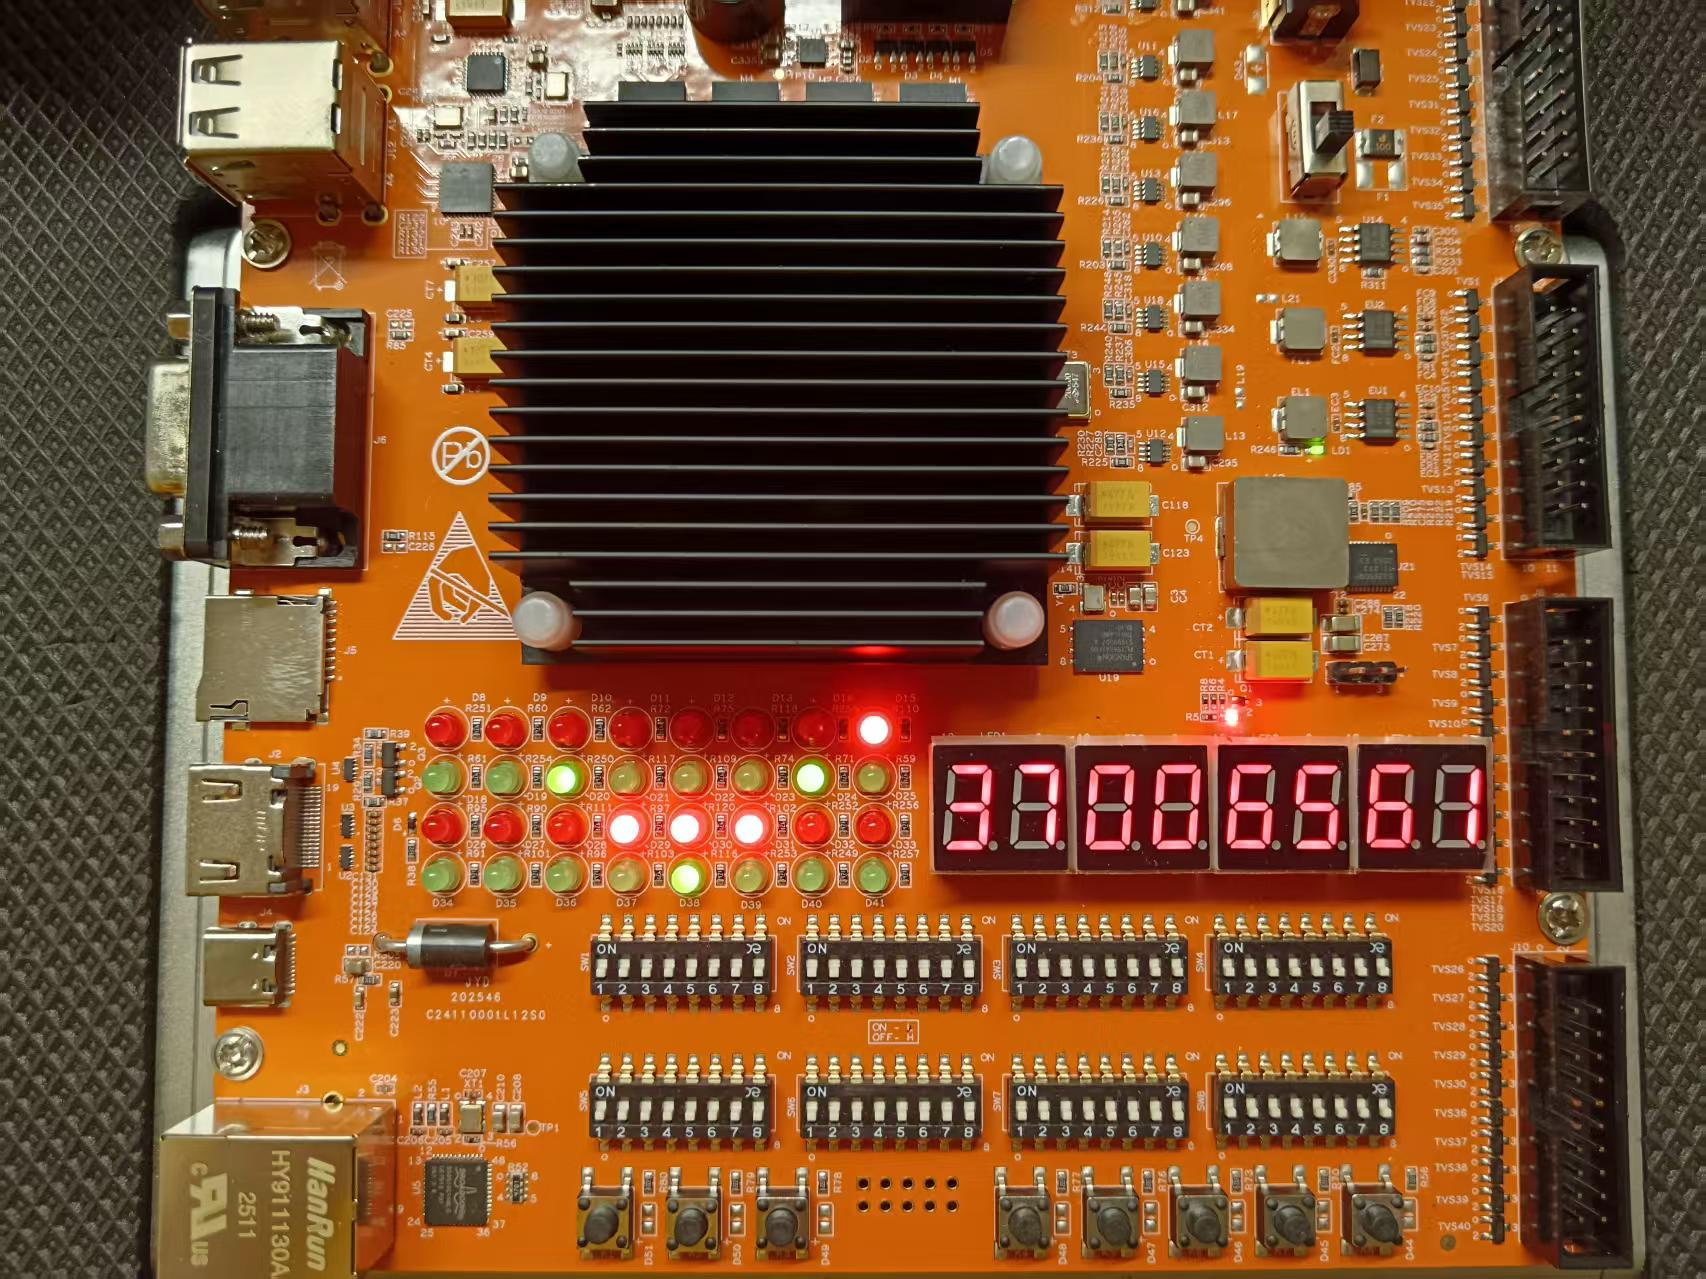
\includegraphics[width=\linewidth,height=0.68\textheight,keepaspectratio]{src0_316m.png}
    \caption*{(a) 以 316.67 MHz 运行 src0}
  \end{minipage}
  \hfill
  \begin{minipage}{0.48\linewidth}
    \centering
    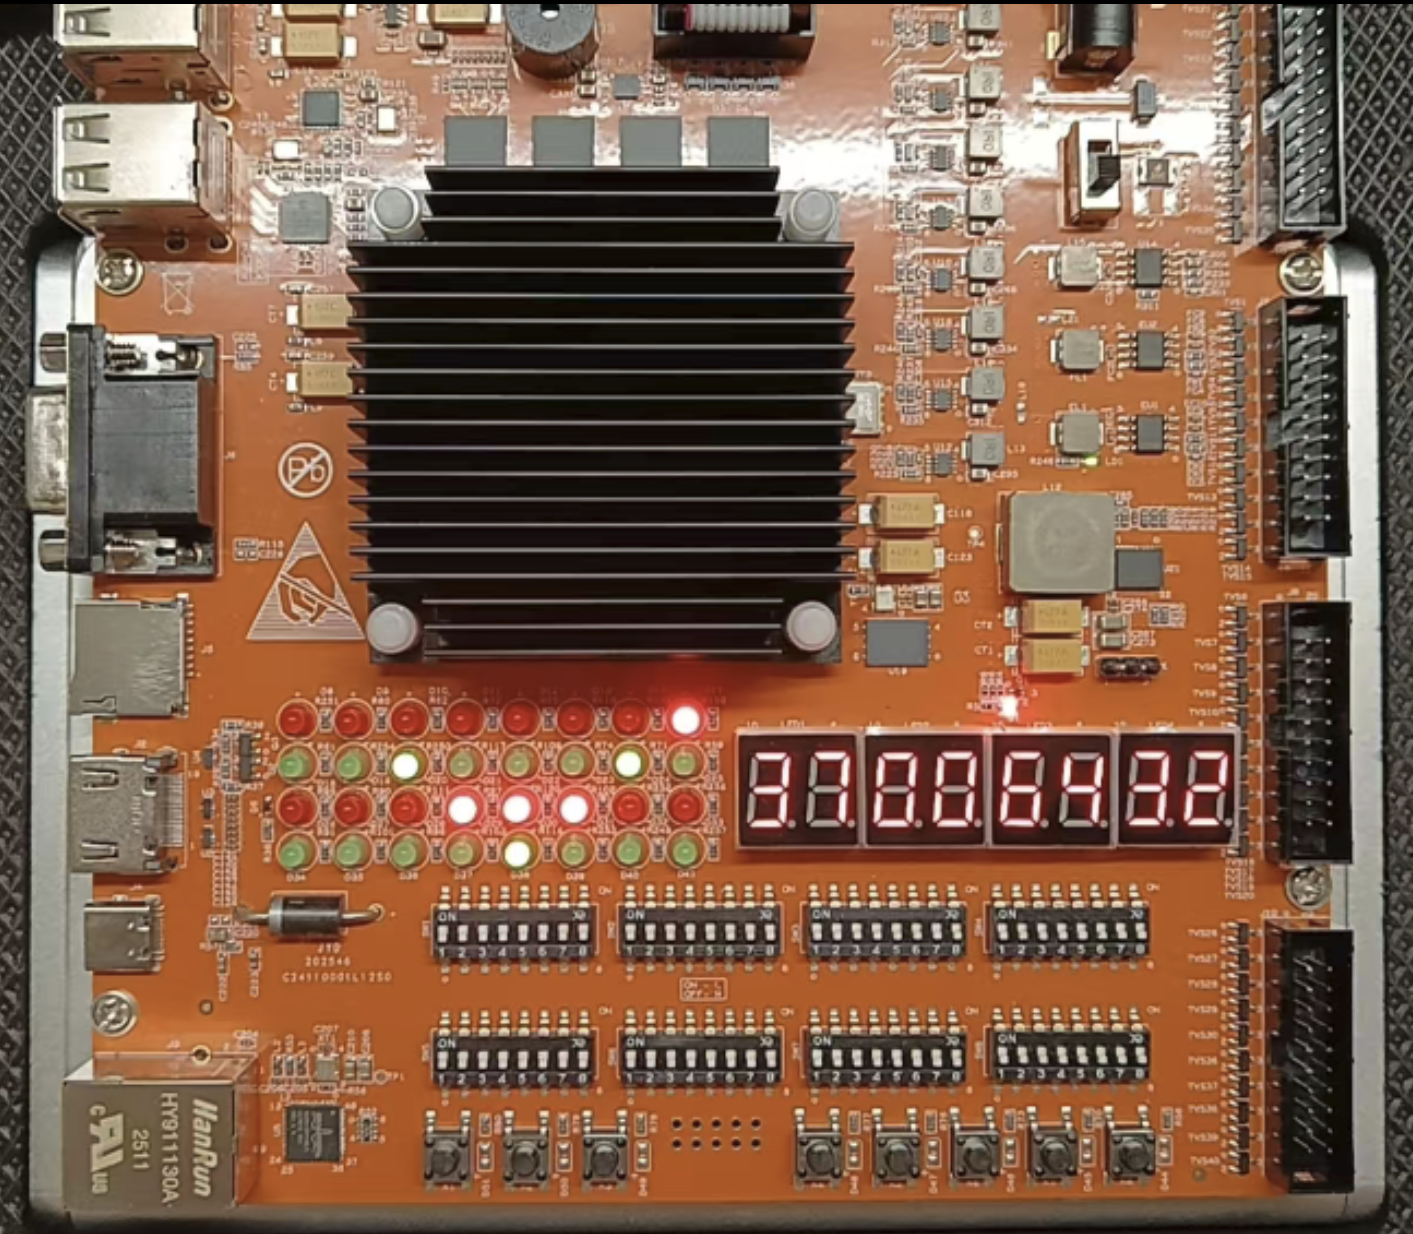
\includegraphics[width=\linewidth,height=0.68\textheight,keepaspectratio]{src1_300m.png}
    \caption*{(b) 以 300.00 MHz 运行 src1}
  \end{minipage}
  \caption{FPGA src0 src1 运行结果}
  \label{fig:src0_1_FPGA}
\end{figure}

\begin{figure}[htbp]
  \centering
  \begin{minipage}{0.48\linewidth}
    \centering
    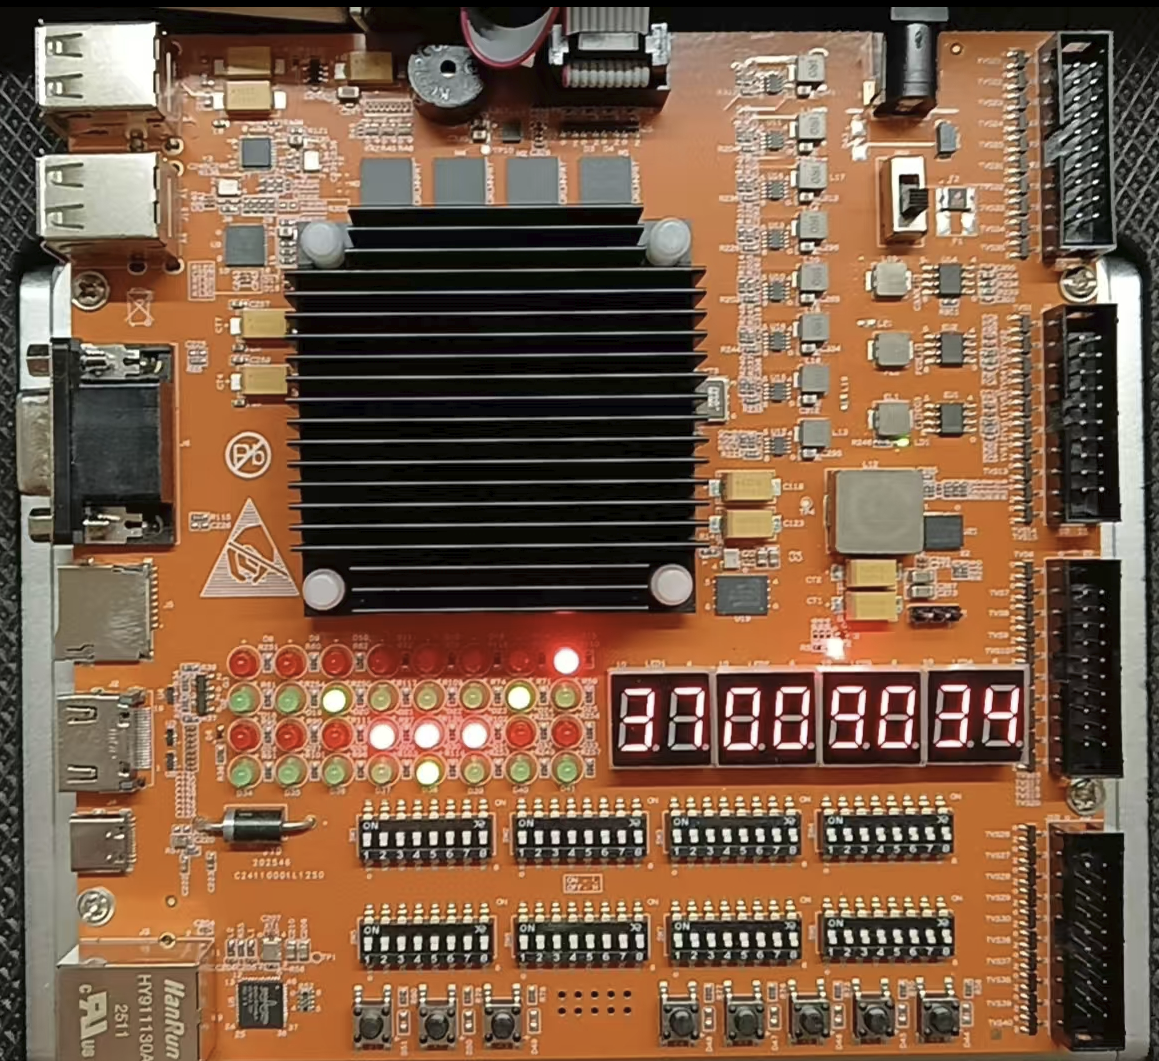
\includegraphics[width=\linewidth,height=0.68\textheight,keepaspectratio]{src2_300m.png}
    \caption*{(a) 以 300.00 MHz 运行 src2}
  \end{minipage}
  \hfill
  \begin{minipage}{0.48\linewidth}
    \centering
    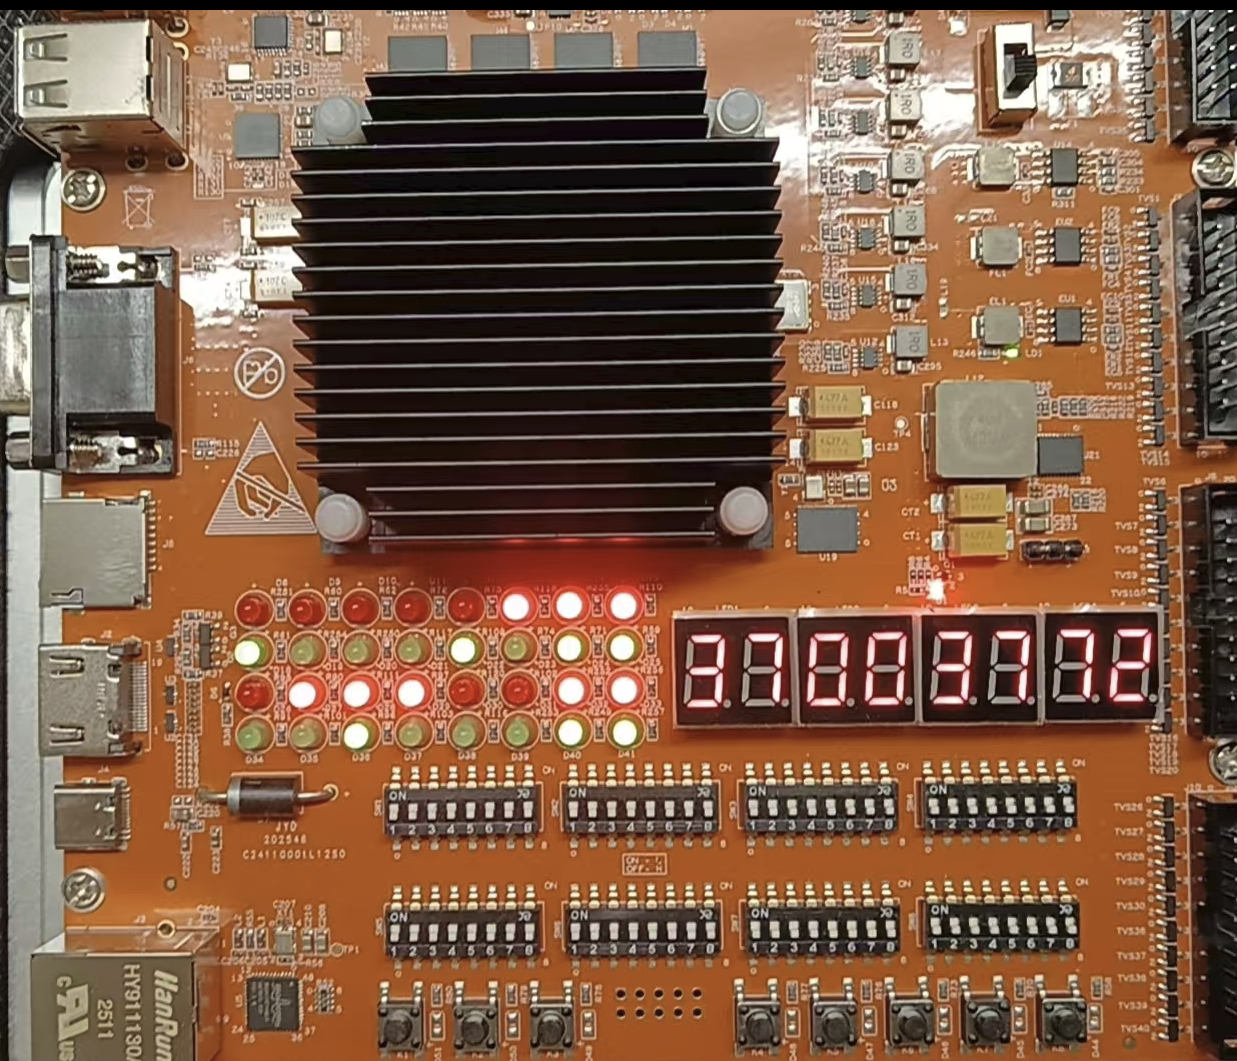
\includegraphics[width=\linewidth,height=0.68\textheight,keepaspectratio]{without_308m.png}
    \caption*{(b) 以 308.00 MHz 运行 withoutMext}
  \end{minipage}
  \caption{FPGA src2 与 withoutMext 运行结果}
  \label{fig:src2_without_FPGA}
\end{figure}

\begin{figure}[htbp]
  \centering
  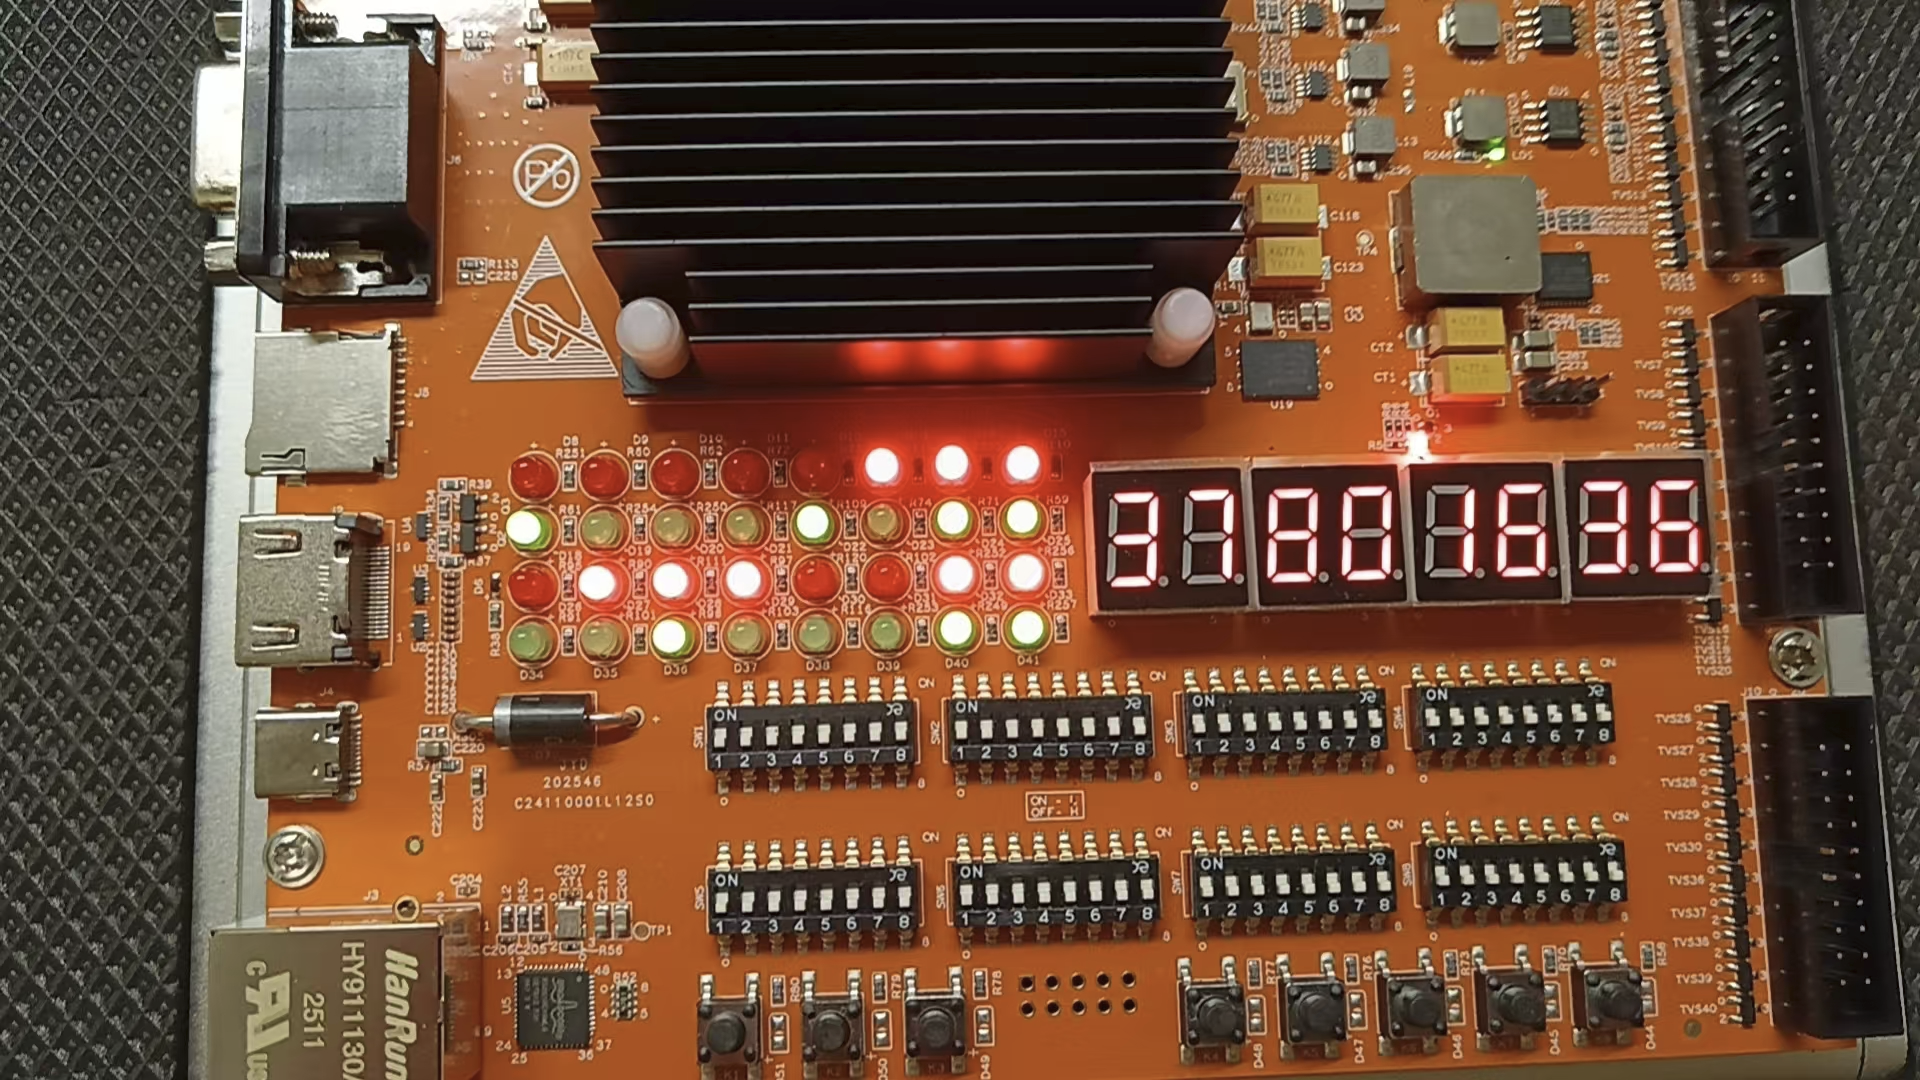
\includegraphics[width=\linewidth,height=0.68\textheight,keepaspectratio]{with_316m.png}
  \caption{以 316.67 MHz 运行 withMext}
  \label{fig:with_FPGA}
\end{figure}

\subparagraph{资源使用及面积、功耗分析}

根据资源和面积报告可知，由于使用了 BRAM 代替了 IROM 和 DRAM，节省了大量的 LUTRAM 使用和面
积占用，故目前的处理器设计使用的资源较少，LUT、FF 仅分别使用了 3\% 和 2\%，
仍有充足余裕可供进一步开发。

\begin{figure}[htbp]
  \centering
  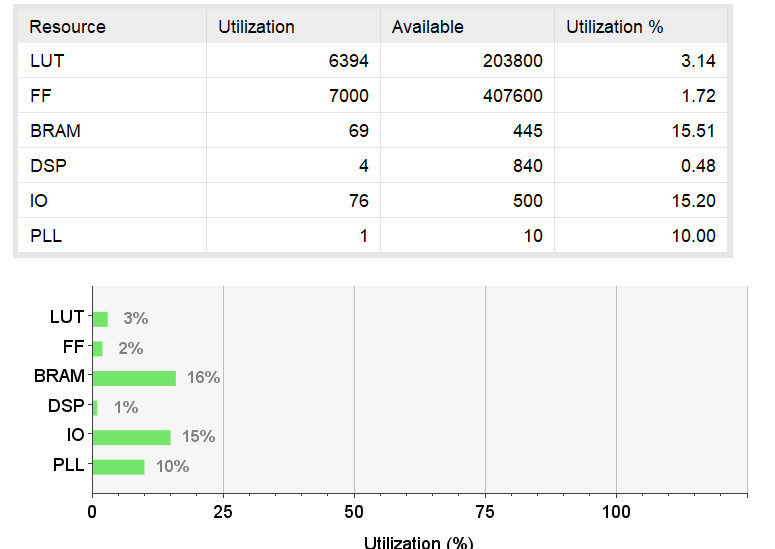
\includegraphics[width=\linewidth,height=0.68\textheight,keepaspectratio]{resources.png}
  \caption{资源使用}
  \label{fig:resource}
\end{figure}

\begin{figure}[htbp]
  \centering
  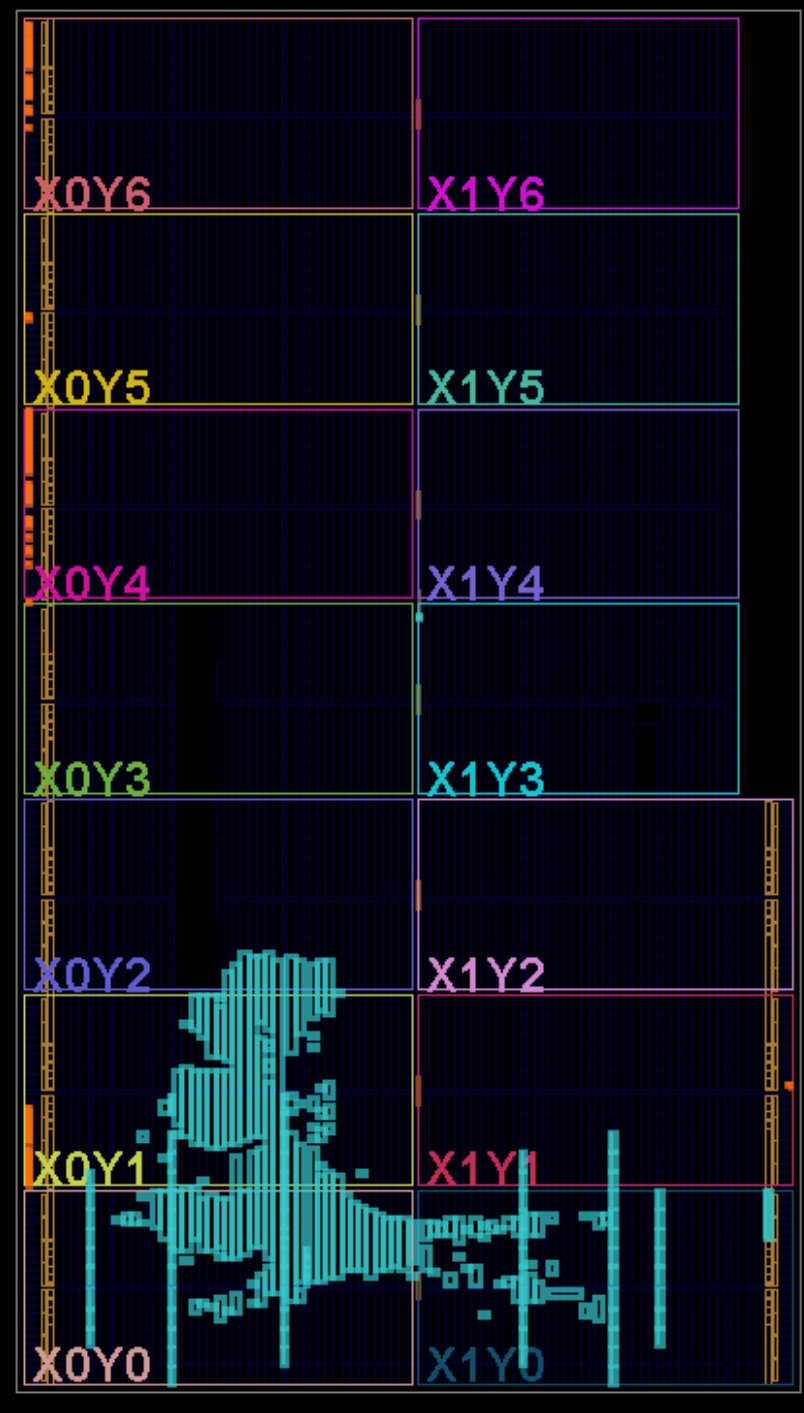
\includegraphics[width=0.82\linewidth,height=0.68\textheight,keepaspectratio]{area.png}
  \caption{综合面积}
  \label{fig:area}
\end{figure}

由功耗报告可知，芯片总功耗为 0.677 W，动态功耗占比为总功耗的 75 \%，静态功耗占比为总功耗的 25\%。而在动态功耗中，Clock、Signals、以及 Logic 的
占比各自为 19\%、29\%和 18\%。具体数据如图~\ref{fig:power} 所示。

\begin{figure}[htbp]
  \centering
  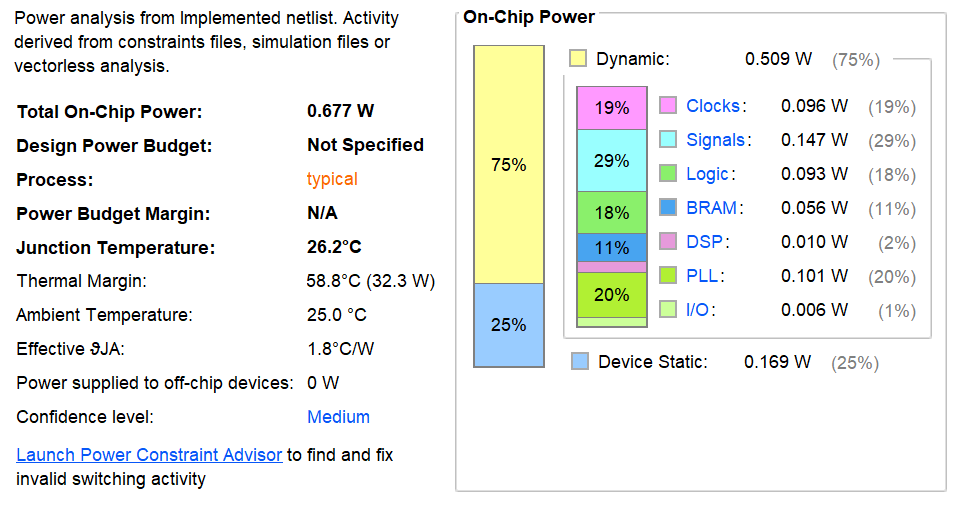
\includegraphics[width=\linewidth,height=0.68\textheight,keepaspectratio]{power.png}
  \caption{功耗占比}
  \label{fig:power}
\end{figure}

\clearpage
\section{总结}
\subsection{可扩展之处}
% 模板限制：300 字内。
后续可完善 RV32F 尚缺的乘除及乘加运算、舍入模式与异常标志，并补充对应回归。
前端可继续优化 BTB 命中、RAS 目标选择与 PC 更新路径，后端可分析 AGU 提前计算带来的 use-load 停顿与 load-use 收益。
工程方面应固化每组测试的 RAS/IP 配置、程序镜像和时序报告，并补充 RV32I 逐条测试截图、整机斜 45 度照片及实测供电功耗。
\subsection{心得体会}
% 模板限制：1000 字内。
高主频设计需要把计算路径、存储器延迟和流水控制放在同一时序框架内考虑。
将 BPU 读表流水化后，提前查询和预测保持必须共同保证请求与响应对齐；仅缩短组合路径，不能自动保证连续取指吞吐。
九级流水线中的数据相关也不能只按指令类型固定停顿，而应结合生产位置和消费需求判断结果能否及时到达。

将 AGU 提前到 ISS 可以减少部分 load-use 停顿，但同时引入紧邻基址依赖的约束；Store Buffer 可以减少写入占用，却需要正确处理同地址合并、读转发和外设顺序。
这些优化说明，局部延迟收益必须在完整程序和统一提交语义下检验。

验证结果还需要区分配置和统计口径。
使用原生 RV32M 的代码流与软件乘除例程具有不同的动态分支行为，不能把两者的准确率差异全部归因于预测器变化。
RAS 收益应在同一镜像下比较；IP 功耗估算、仿真周期与板卡运行时间也应分别记录。
保留配置、日志和照片，使功能、时序及性能结论能够对应到具体工程状态，是处理器持续演进的重要基础。

\begingroup
\small
\setstretch{1.1}
\begin{thebibliography}{9}
  \bibitem{smith1981study}
  James E. Smith. A Study of Branch Prediction Strategies. In \emph{Proceedings of the 8th
  Annual Symposium on Computer Architecture}, pages 135--148. IEEE Computer Society Press, 1981.

  \bibitem{mittal2019survey}
  Sparsh Mittal. A Survey of Techniques for Dynamic Branch Prediction. \emph{Concurrency and
  Computation: Practice and Experience}, 31(1):e4666, 2019.

  \bibitem{smith1995microarchitecture}
  James E. Smith and Gurindar S. Sohi. The Microarchitecture of Superscalar Processors.
  \emph{Proceedings of the IEEE}, 83(12):1609--1624, 1995.
\end{thebibliography}
\endgroup


\end{document}
